% -*- Mode:TeX -*-

%% The documentclass options along with the pagestyle can be used to generate
%% a technical report, a draft copy, or a regular thesis.  You may need to
%% re-specify the pagestyle after you \include  cover.tex.  For more
%% information, see the first few lines of mitthesis.cls. 

%\documentclass[12pt,vi,twoside]{mitthesis}
%%
%%  If you want your thesis copyright to you instead of MIT, use the
%%  ``vi'' option, as above.
%%
%\documentclass[12pt,twoside,leftblank]{mitthesis}
%%
%% If you want blank pages before new chapters to be labelled ``This
%% Page Intentionally Left Blank'', use the ``leftblank'' option, as
%% above. 

\documentclass[10pt,twoside]{mitthesis}
\usepackage{lgrind}
\usepackage{xcolor}
\usepackage{hyperref}
\usepackage{graphicx}
\usepackage{wrapfig}
\usepackage{listings}
\usepackage{color}
\usepackage{setspace}
\newcommand\todo[1]{\textcolor{red}{#1}}
%\newcommand\syntax[1]{\textcolor{blue}{#1}}
\pagestyle{plain}


\definecolor{mygreen}{rgb}{0,0.6,0}
\definecolor{mygray}{rgb}{0.5,0.5,0.5}
\definecolor{mymauve}{rgb}{0.58,0,0.82}
\definecolor{black}{rgb}{0,0,0}

\lstset{ %
  backgroundcolor=\color{white},   % choose the background color; you must add \usepackage{color} or \usepackage{xcolor}
  basicstyle=\scriptsize\ttfamily,        % the size of the fonts that are used for the code
  breakatwhitespace=false,         % sets if automatic breaks should only happen at whitespace
  breaklines=true,                 % sets automatic line breaking
  captionpos=b,                    % sets the caption-position to bottom
  commentstyle=\color{mygreen},    % comment style
  deletekeywords={...},            % if you want to delete keywords from the given language
  escapeinside={\%*}{*)},          % if you want to add LaTeX within your code
  extendedchars=true,              % lets you use non-ASCII characters; for 8-bits encodings only, does not work with UTF-8
  frame=single,                    % adds a frame around the code
  keepspaces=true,                 % keeps spaces in text, useful for keeping indentation of code (possibly needs columns=flexible)
  keywordstyle=\color{blue},       % keyword style
  %language=Octave,                 % the language of the code
  morekeywords={*,...},            % if you want to add more keywords to the set
  numbers=left,                    % where to put the line-numbers; possible values are (none, left, right)
  numbersep=5pt,                   % how far the line-numbers are from the code
  numberstyle=\tiny\color{mygray}, % the style that is used for the line-numbers
  rulecolor=\color{black},         % if not set, the frame-color may be changed on line-breaks within not-black text (e.g. comments (green here))
  showspaces=false,                % show spaces everywhere adding particular underscores; it overrides 'showstringspaces'
  showstringspaces=false,          % underline spaces within strings only
  showtabs=false,                  % show tabs within strings adding particular underscores
  stepnumber=2,                    % the step between two line-numbers. If it's 1, each line will be numbered
  stringstyle=\color{black},     % string literal style
  tabsize=2,                       % sets default tabsize to 2 spaces
  title=\lstname                   % show the filename of files included with \lstinputlisting; also try caption instead of title
}

%% This bit allows you to either specify only the files which you wish to
%% process, or `all' to process all files which you \include.
%% Krishna Sethuraman (1990).

\begin{document}

% -*-latex-*-
% 
% For questions, comments, concerns or complaints:
% thesis@mit.edu
% 
%
% $Log: cover.tex,v $
% Revision 1.8  2008/05/13 15:02:15  jdreed
% Degree month is June, not May.  Added note about prevdegrees.
% Arthur Smith's title updated
%
% Revision 1.7  2001/02/08 18:53:16  boojum
% changed some \newpages to \cleardoublepages
%
% Revision 1.6  1999/10/21 14:49:31  boojum
% changed comment referring to documentstyle
%
% Revision 1.5  1999/10/21 14:39:04  boojum
% *** empty log message ***
%
% Revision 1.4  1997/04/18  17:54:10  othomas
% added page numbers on abstract and cover, and made 1 abstract
% page the default rather than 2.  (anne hunter tells me this
% is the new institute standard.)
%
% Revision 1.4  1997/04/18  17:54:10  othomas
% added page numbers on abstract and cover, and made 1 abstract
% page the default rather than 2.  (anne hunter tells me this
% is the new institute standard.)
%
% Revision 1.3  93/05/17  17:06:29  starflt
% Added acknowledgements section (suggested by tompalka)
% 
% Revision 1.2  92/04/22  13:13:13  epeisach
% Fixes for 1991 course 6 requirements
% Phrase "and to grant others the right to do so" has been added to 
% permission clause
% Second copy of abstract is not counted as separate pages so numbering works
% out
% 
% Revision 1.1  92/04/22  13:08:20  epeisach

% NOTE:
% These templates make an effort to conform to the MIT Thesis specifications,
% however the specifications can change.  We recommend that you verify the
% layout of your title page with your thesis advisor and/or the MIT 
% Libraries before printing your final copy.
\title{Algorithmic Craft: Tools and Practices For Creating Useful and Decorative Objects With Code}

\author{Jennifer Jacobs}
% If you wish to list your previous degrees on the cover page, use the 
% previous degrees command:
%       \prevdegrees{A.A., Harvard University (1985)}
% You can use the \\ command to list multiple previous degrees
%       \prevdegrees{B.S., University of California (1978) \\
%                    S.M., Massachusetts Institute of Technology (1981)}
\department{Department of Media Arts and Sciences}

% If the thesis is for two degrees simultaneously, list them both
% separated by \and like this:
% \degree{Doctor of Philosophy \and Master of Science}
\degree{Masters of Science}

% As of the 2007-08 academic year, valid degree months are September, 
% February, or June.  The default is June.
\degreemonth{June}
\degreeyear{2013}
\thesisdate{June something, 2013}

%% By default, the thesis will be copyrighted to MIT.  If you need to copyright
%% the thesis to yourself, just specify the `vi' documentclass option.  If for
%% some reason you want to exactly specify the copyright notice text, you can
%% use the \copyrightnoticetext command.  
%\copyrightnoticetext{\copyright IBM, 1990.  Do not open till Xmas.}

% If there is more than one supervisor, use the \supervisor command
% once for each.
\supervisor{Leah Buechley}{Associate Professor of Media Arts and Sciences}
\supervisor{Mitchel Resnick}{ Academic Head, Program in Media Arts and Sciences}
\supervisor{Neri Oxman}{Assistant Professor of Media Arts and Sciences}

% This is the department committee chairman, not the thesis committee
% chairman.  You should replace this with your Department's Committee
% Chairman.
\chairman{...}{Chairman, Department Committee on Graduate Theses}

% Make the titlepage based on the above information.  If you need
% something special and can't use the standard form, you can specify
% the exact text of the titlepage yourself.  Put it in a titlepage
% environment and leave blank lines where you want vertical space.
% The spaces will be adjusted to fill the entire page.  The dotted
% lines for the signatures are made with the \signature command.
\maketitle

% The abstractpage environment sets up everything on the page except
% the text itself.  The title and other header material are put at the
% top of the page, and the supervisors are listed at the bottom.  A
% new page is begun both before and after.  Of course, an abstract may
% be more than one page itself.  If you need more control over the
% format of the page, you can use the abstract environment, which puts
% the word "Abstract" at the beginning and single spaces its text.

%% You can either \input (*not* \include) your abstract file, or you can put
%% the text of the abstract directly between the \begin{abstractpage} and
%% \end{abstractpage} commands.

% First copy: start a new page, and save the page number.
\cleardoublepage
% Uncomment the next line if you do NOT want a page number on your
% abstract and acknowledgments pages.
% \pagestyle{empty}
\setcounter{savepage}{\thepage}
\begin{abstractpage}
% $Log: abstract.tex,v $
% Revision 1.1  93/05/14  14:56:25  starflt
% Initial revision
% 
% Revision 1.1  90/05/04  10:41:01  lwvanels
% Initial revision
% 
%
%% The text of your abstract and nothing else (other than comments) goes here.
%% It will be single-spaced and the rest of the text that is supposed to go on
%% the abstract page will be generated by the abstractpage environment.  This
%% file should be \input (not \include 'd) from cover.tex.
The accessibility, diversity, and functionality of modern computer systems make computer programming useful in many realms of human study and advancement. Visual and physical art, craft, and design are interrelated domains that offer exciting possibilities when combined with programming. Unfortunately, the use of programming is currently limited as a medium for art and design for young people and amateur programmers. Many potential users view programming as highly specialized, difficult, inaccessible, and only relevant as a career path in science, engineering, or business fields, rather than as a mode of personal expression. Despite this perception, programming has the potential to correspond well with physical craft practices. By forging a strong connections between programming and the construction of personally relevant physical objects, it may be possible to foster meaningful creative experiences for non-professionals. The term algorithmic craft describes the combination of computational design, digital fabrication and craft to create functional artifacts. This thesis describes my work in developing a set of software tools that attempt to make the practice of algorithmic craft accessible for novice programers. Through it, I describe the design of each tool and discuss my experiences in engaging people in the creation of objects that are designed with programming, formed by machines, and shaped by hand. 
\end{abstractpage}


%% ----------------------------------------------------------------
% The "Funny Quote Page"
\pagestyle{empty}  % No headers or footers for the following pages

\null\vfill
% Now comes the "Funny Quote", written in italics
\textit{``The type of work which modern technology is most successful in reducing or even eliminating is skillful, productive work of human hands, in touch with real materials of one kind or another. In an advanced industrial society, such work has become exceedingly rare. A great part of the modern neurosis may be due to this very fact; for the human being enjoys nothing more to be creatively, usefully, productively engaged with both his hands and his brains."
}

\begin{flushright}
E.F. Schumacher, Small is Beautiful (1973)
\end{flushright}

\vfill\vfill\vfill\vfill\vfill\vfill\null
\clearpage  % Funny Quote page ended, start a new page
%% ----------------------------------------------------------------


% Additional copy: start a new page, and reset the page number.  This way,
% the second copy of the abstract is not counted as separate pages.
% Uncomment the next 6 lines if you need two copies of the abstract
% page.
% \setcounter{page}{\thesavepage}
% \begin{abstractpage}
% % $Log: abstract.tex,v $
% Revision 1.1  93/05/14  14:56:25  starflt
% Initial revision
% 
% Revision 1.1  90/05/04  10:41:01  lwvanels
% Initial revision
% 
%
%% The text of your abstract and nothing else (other than comments) goes here.
%% It will be single-spaced and the rest of the text that is supposed to go on
%% the abstract page will be generated by the abstractpage environment.  This
%% file should be \input (not \include 'd) from cover.tex.
The accessibility, diversity, and functionality of modern computer systems make computer programming useful in many realms of human study and advancement. Visual and physical art, craft, and design are interrelated domains that offer exciting possibilities when combined with programming. Unfortunately, the use of programming is currently limited as a medium for art and design for young people and amateur programmers. Many potential users view programming as highly specialized, difficult, inaccessible, and only relevant as a career path in science, engineering, or business fields, rather than as a mode of personal expression. Despite this perception, programming has the potential to correspond well with physical craft practices. By forging a strong connections between programming and the construction of personally relevant physical objects, it may be possible to foster meaningful creative experiences for non-professionals. The term algorithmic craft describes the combination of computational design, digital fabrication and craft to create functional artifacts. This thesis describes my work in developing a set of software tools that attempt to make the practice of algorithmic craft accessible for novice programers. Through it, I describe the design of each tool and discuss my experiences in engaging people in the creation of objects that are designed with programming, formed by machines, and shaped by hand. 
% \end{abstractpage}

\cleardoublepage

\section*{Acknowledgments}

To come....

%%%%%%%%%%%%%%%%%%%%%%%%%%%%%%%%%%%%%%%%%%%%%%%%%%%%%%%%%%%%%%%%%%%%%%
% -*-latex-*-

\pagestyle{plain}
  % -*- Mode:TeX -*-
%% This file simply contains the commands that actually generate the table of
%% contents and lists of figures and tables.  You can omit any or all of
%% these files by simply taking out the appropriate command.  For more
%% information on these files, see appendix C.3.3 of the LaTeX manual. 
\tableofcontents
\newpage
\listoffigures
\newpage
\listoftables


%% This is an example first chapter.  You should put chapter/appendix that you
%% write into a separate file, and add a line \include{yourfilename} to
%% main.tex, where `yourfilename.tex' is the name of the chapter/appendix file.
%% You can process specific files by typing their names in at the 
%% \files=
%% prompt when you run the file main.tex through LaTeX.
\chapter{Introduction}

Computation is a driving force in our world. The power and ubiquity of  modern computer systems have made the skill of computer programming (hereafter programming) relevant to a wide range of human studies and disciplines. Most commonly, programming is viewed as an essential component of science, engineering, and business related applications\cite{resnick1}. As a result, many nascent programmers view programming as highly specialized, difficult, inaccessible, and only relevant as a career path in those particular fields. In reality, computation is a broad discipline with many applications, ranging from professional to personal. Foremost programing can serve as a medium for personal expression, through applications in art and design. With the emergence of digital fabrication technology, In addition, programing provides the means to design and produce useful objects and devices, not only on at an industrial scale, but also on a personal and individual scale \cite{mellis_thesis}. When programing is used create unique, functional physical objects, new possibilities emerge in the way people design,  the types of objects people create, and role programing can play in peoples' lives.  Computational design, the practice of programming to create form, structure and ornamentation, is a new way to design. When paired with digital fabrication technology, computational design allows people to make physical objects by writing code. My objective is to examine the combination of computational design, digital fabrication and traditional arts and crafts for the production of functional decorative objects. I define this domain with the term algorithmic craft. The process of bridging the spaces between textual programming language, visual design, and physical construction however, is not self-evident and raises many practical and theoretical questions.  What are the important design principles to consider when creating  programming environments for physical design? How do we compellingly link textual code with visual designs and what are the appropriate intersection points between textual manipulation and visual manipulation? What support is required to help people move back and forth from programming to building real objects in a way that is comfortable, expressive and pleasurable? How can we remove the technical challenges in translating code into an object that can be successfully fabricated, while still supporting a wide variety of design styles, aesthetics and approaches? Finally, how can we interlink the often disparate processes of physical prototyping with digital design and programming in a way that creatively reinforces both physical and virtual modes of working?

This thesis explores the affordances of algorithmic craft as a form of casual creative engagement in programing, craft and fabrication. As a part of my study of algorithmic craft, I developed three different software tools to support practitioners in this domain: Codeable Objects, Soft Objects and DressCode. Codeable objects is a programing library that helps people design and fabricate laser-cut lamps. Soft Objects is an extension of Codeable Objects that allows people to use programing to create forms and patterns for fashion and garment design. Finally DressCode is a combined graphic design and programing environment with a custom programing language developed to support open-ended computational design for digital fabrication. Each of these tools were evaluated in workshops where people used them in combination with 2-axis fabrication machines to produce physical artifacts. Through the workshops, I examined different approaches to combining programing and visual design for novice programmers. In addition, I evaluated how the materials and approaches of various crafting techniques could be combined with the form and structure of Computer Aided Design (CAD). The lessons learned in each workshop were used to inform the development of the following tool. This thesis presents the evolution of these three tools, and demonstrates the rationale their design through user testing and feedback. I conclude with a discussion of some of the unique affordances of Algorithmic Craft, and the possibilities it offers for how we design, construct and craft artifacts in years to come.


%% This is an example first chapter. You should put chapter/appendix that you
%% write into a separate file, and add a line \include{yourfilename} to
%% main.tex, where `yourfilename.tex' is the name of the chapter/appendix file.
%% You can process specific files by typing their names in at the 
%% \files=
%% prompt when you run the file main.tex through LaTeX.
\chapter{Background and Motivation}

\begin{flushright}
\textit{``The mathematician's patterns, like the painter's or the poet's 
must be beautiful; the ideas like the colours or the words, must fit 
together in a harmonious way. Beauty is the first test: there is no 
permanent place in the world for ugly mathematics."
}
G. H. Hardy \cite{hardy}
\end{flushright}


In order to illustrate the creative potential of algorithmic craft, it is useful to examine its contents: computational design, digital fabrication and craft. Each has distinct strengths and limitations. Through their convergence, new, compelling forms of creation become possible. In computational design, the abstract qualities of computation provide a powerful way of thinking about design. With appropriate programming, a computer can embody any conceivable process \cite{mateas}. Similarly, computational design can be applied to any design domain, be it physical, visual, sonic, or interactive. Although individual applications of computational design often consider material properties that are relevant to a specific domain, computational design does possess an inherent connection to the material world. Craft on the other hand is closely linked to materiality. Craftspeople work in close contact with the physical world and craft artifacts and processes are directly informed by material properties. Digital fabrication provides a connection between the abstraction of computational design and the material domain of craft by converting digital concepts to physical forms. In the following section I discuss the properties of computational design, digital fabrication and craft in greater detail and describe connection points between each discipline.

 \begin{center}
\begin{figure}[h!]
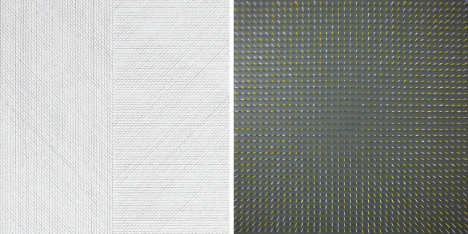
\includegraphics[width=\columnwidth]{images/wall_drawings.jpg}
\caption{Wall drawings by Sol Lewitt. From left to right: Wall Drawing 19: A wall divided vertically into six equal parts, with two of the four kinds of line directions superimposed in each part (1969), Wall Drawing 38 (Detail): Tissue paper cut into 1.5-inch (4 cm) squares and inserted into holes in the gray pegboard walls. All holes in the walls are filled randomly (1970).}
\label{fig:wall_drawings}
\end{figure}
\end{center}

\section{Computational Design}\label{sec:computational_design}
As previously mentioned, computational design can refer to a range of design practices that incorporate computational processes. Computational processes are explicit patterns of rules that can manipulate data \cite{abelson}. Computer programs are description of computational processes in a format that is readable by a computer. My focus in computational design is the process of using computation processes to create visual forms and patterns. Because computational design usually requires the designer to write programs, it is possible to mistake the practice of computational design as a technical skill rather than a way of thinking \cite{reas}. It is true that computational design requires a degree of technical expertise; practitioners must be able to write and read code. Despite this requirement, computational design is better represented as a way of applying procedural thinking to a design task. Rather than producing specific design representations, the designer authors a set of rules that define a system capable of producing many outcomes. Designs are presented in abstract terms, resulting in the potential to create multiple variations that share a set of constraints. One of the challenges of computational design is in authoring guidelines that effectively produce solutions within the desired design space. Presented as an ordered set of instructions, these guidelines constitute an algorithm. Arguably, it is possible to engage in computational design without using a computer. The artist Sol Lewitt created a number of artworks consisting of a set of instructions that dictated the constraints of an artwork:

\begin{quotation}
WORK FROM INSTRUCTIONS (1971):
\\USING A BLACK, HARD CRAYON DRAW A TWENTY INCH SQUARE.
\\DIVIDE THIS SQUARE INTO ONE INCH SQUARES.
 \\WITHIN EACH ONE INCH SQUARE, DRAW NOTHING, OR DRAW A DIAGONAL STRAIGHT LINE FROM CORNER TO CORNER OR TWO CROSSING STRAIGHT LINES DIAGONALLY FROM CORNER TO CORNER.
\end{quotation}

 The resulting piece would vary depending on how the instructions were interpreted by the people executing them. Many of his other artworks contained the instructions for producing them in the title of the piece (figure:\ref{fig:wall_drawings}.) Using a computer to execute computational design algorithms instead of human beings greatly accelerates the process of execution, and supports a non-linear design process. The specific affordances of computational design are as follows:
 
\begin{itemize}
\item \textbf{Precision:} Computation supports high levels of numerical precision with relatively little effort on the part of the designer.

\begin{center}
\begin{figure}[h!]
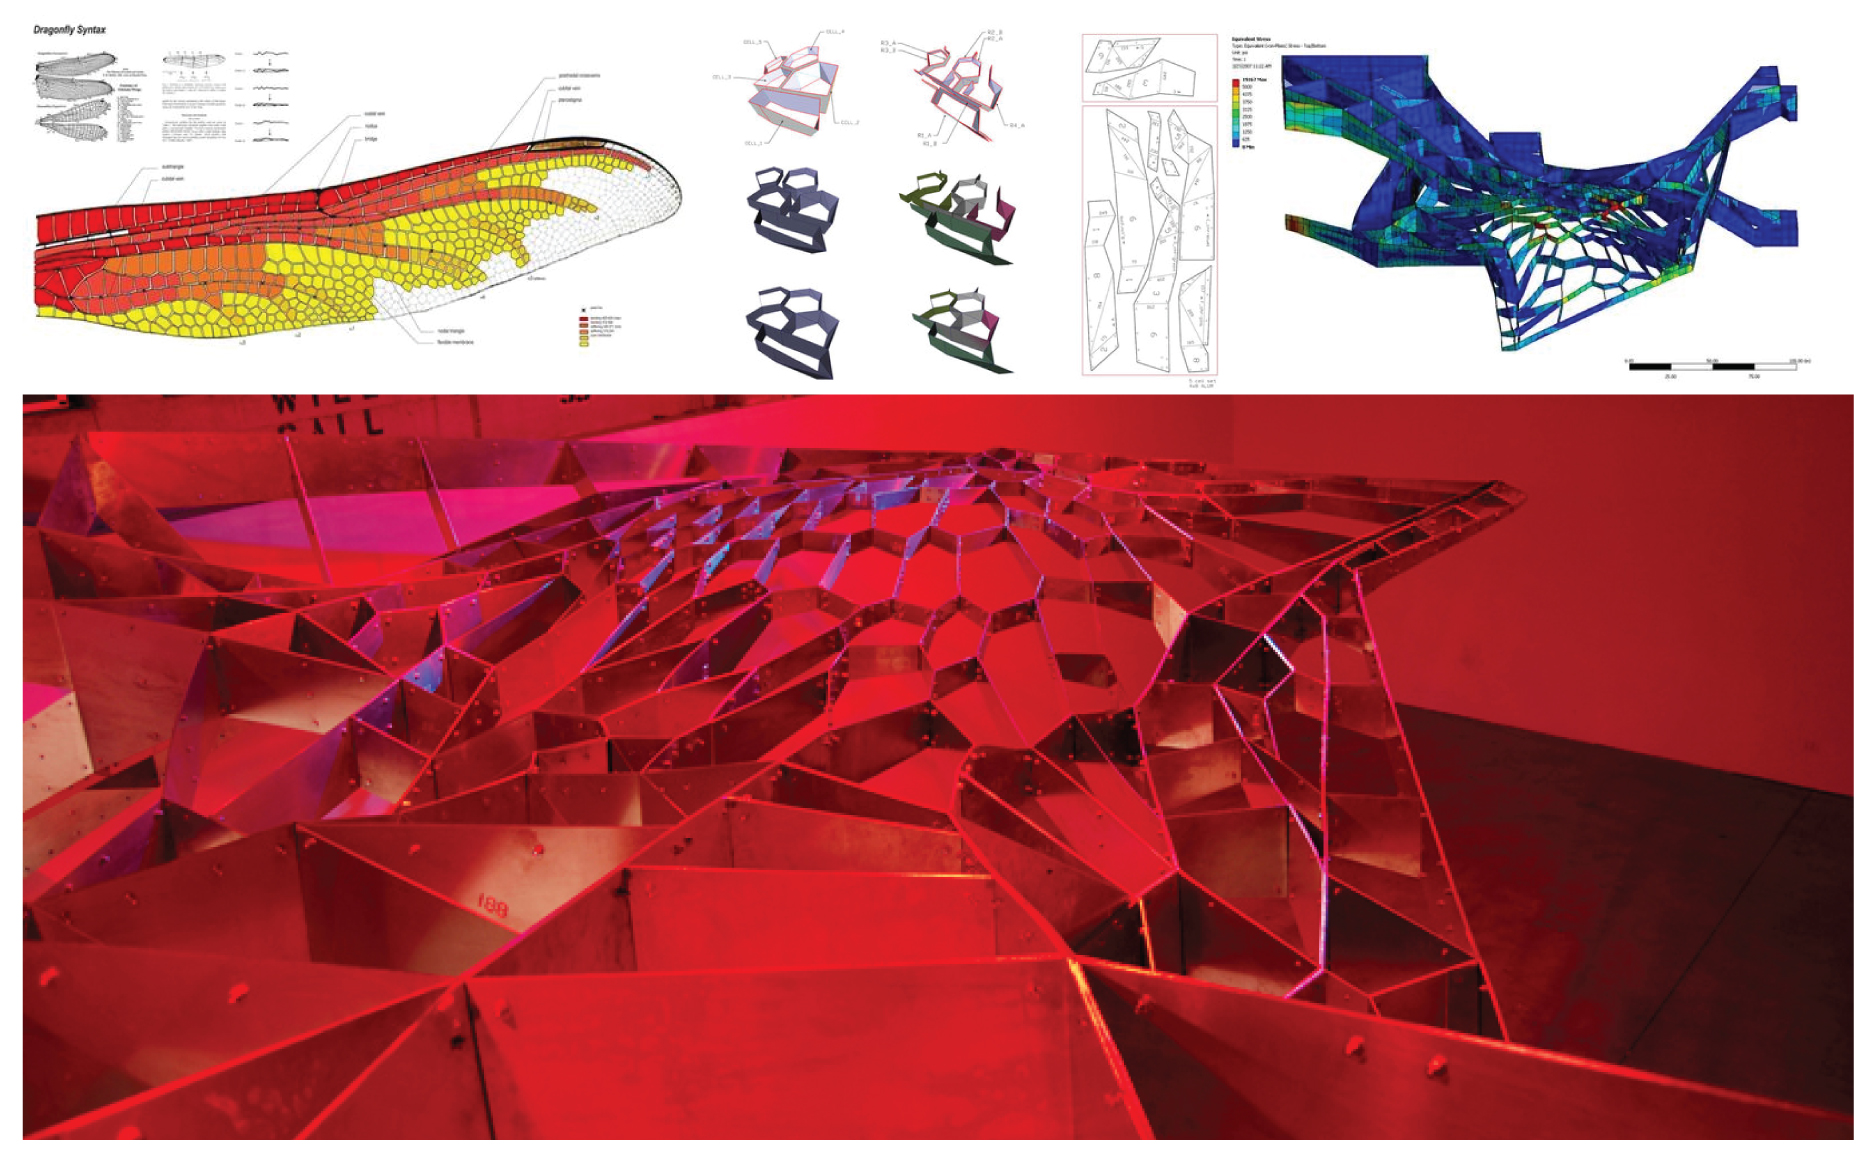
\includegraphics[width=\columnwidth]{images/dragonfly.jpg}
\caption{Dragonfly by EMERGENT/ Tom Wiscombe (2007). Installation. Inspired by the structure of a dragonfly wing, this installation was shaped in by a set of parameters including gravity, specific support points and flat material properties. The structure was generated based on support and loading data, which were run through a feedback loop, producing a design that supported both the performance criteria and a novel variation of form \cite{dunn}. }
\label{fig:dragonfly}
\end{figure}
\end{center}

\item \textbf{Visual Complexity:} Computational design supports the creation and transformation of complex patterns and structures through rapid automation and iteration which allows for the combination and manipulation of large numbers of simple elements in a structured manner. 

\begin{center}
\begin{figure}[h!]
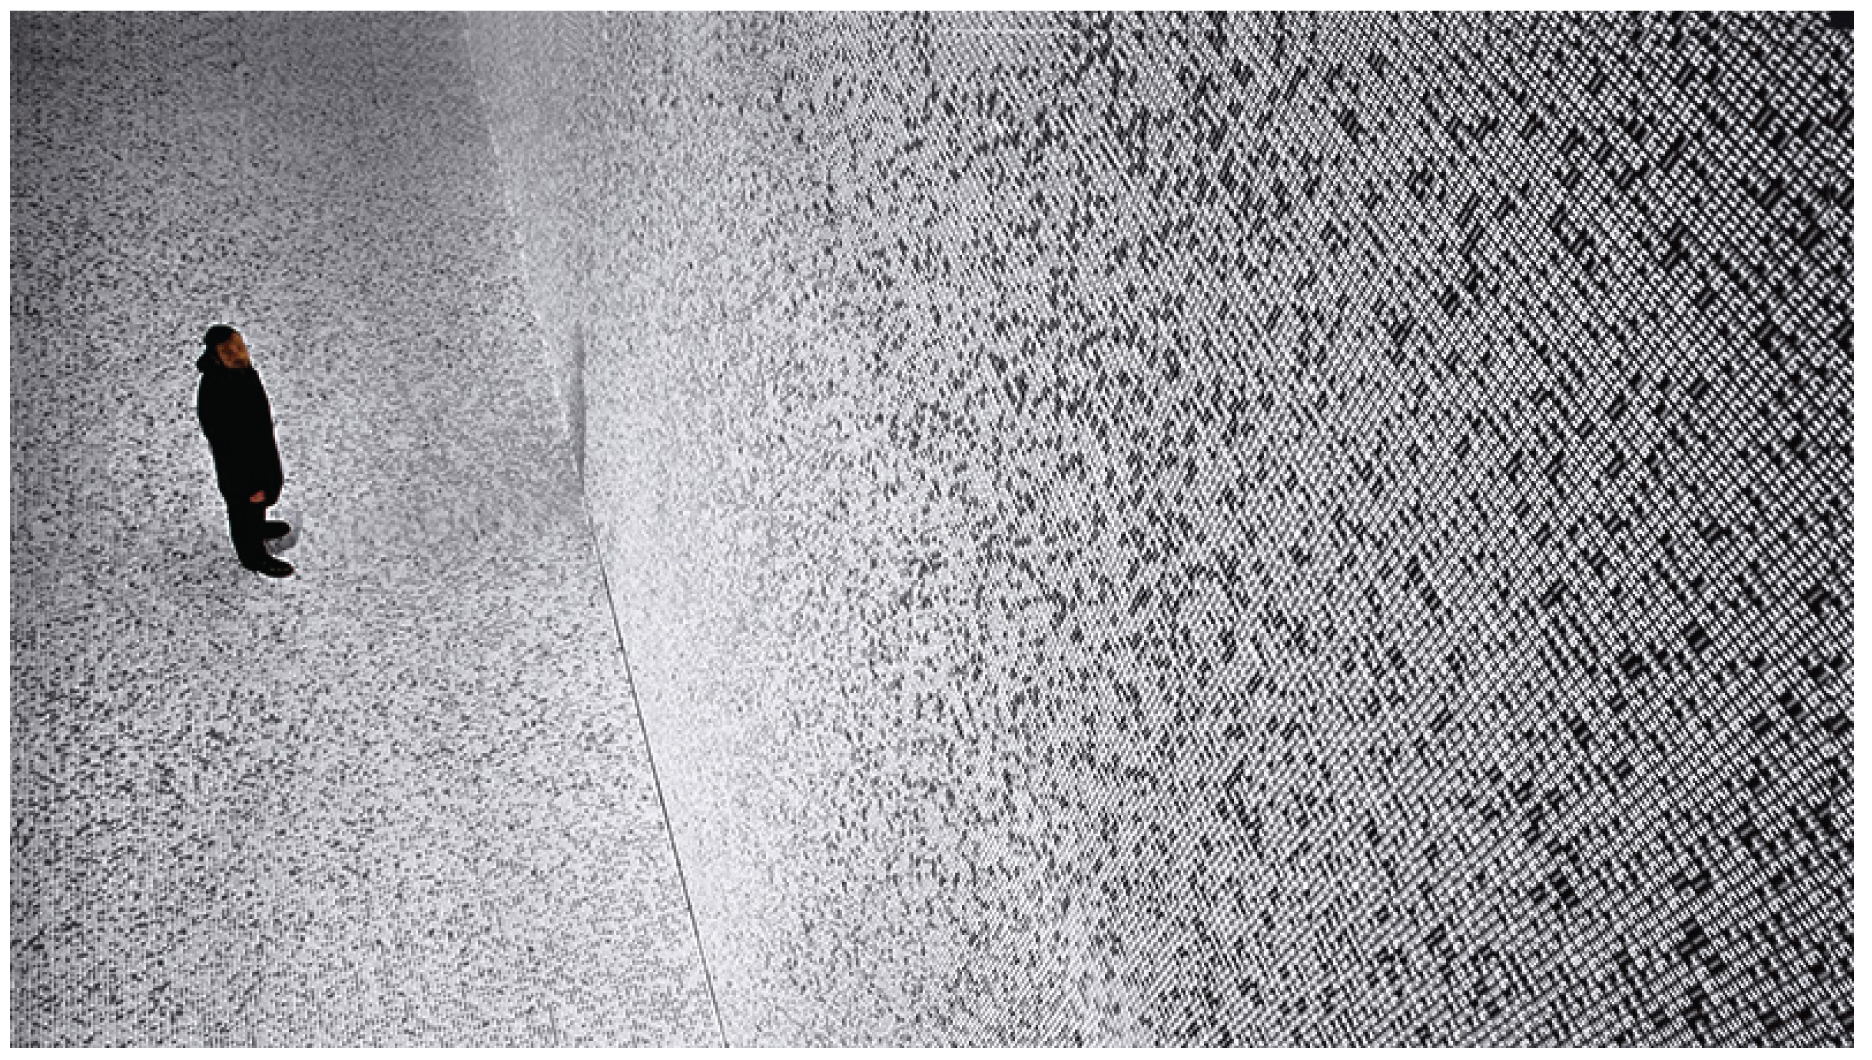
\includegraphics[width=\columnwidth]{images/ikeda.jpg}
\caption{data.tron by Ryoji Ikeda (2008). Dynamic computer visual and sound installation. Each pixel of the visual image is dynamically calculated as a visualization of data from hard drive errors and software code. \cite{ikeda_website}. }
\label{fig:ikeda}
\end{figure}
\end{center}

\item \textbf{Generativity and randomness:} Computation allows for the programmer to create algorithms, which when run, allow for the computer to autonomously produce unique and often unexpected designs.

 \begin{center}
\begin{figure}[h!]
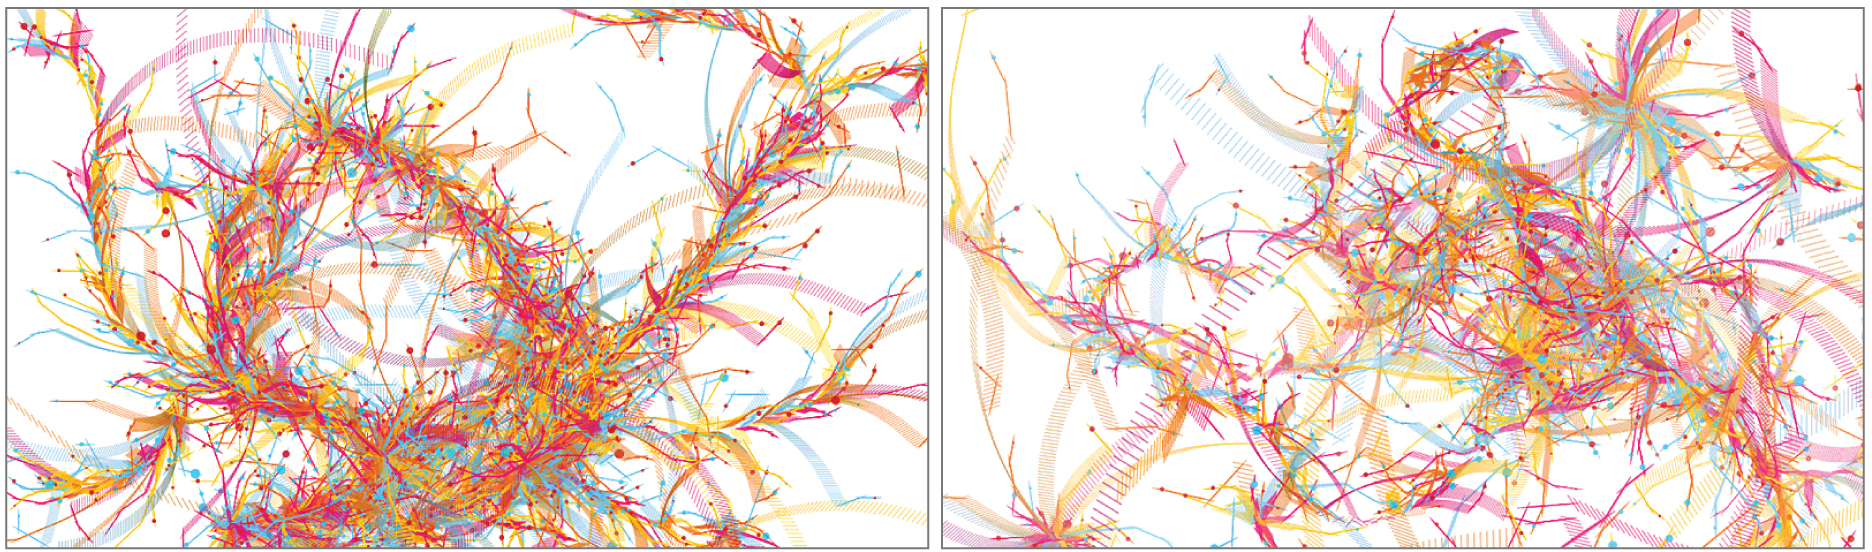
\includegraphics[width=\columnwidth]{images/marius_watz.jpg}
\caption{Abstract01.js by Marius Watz (2010). Interactive. The piece is comprised of a Javascript program that autonomously creates unique abstract compositions based on a set of visual guidelines specified by the artist \cite{watz_website}.}
\label{fig:marius_watz}
\end{figure}
\end{center}

\item \textbf{Parameterization:} Computation allows users to specify a set of degrees of freedom and constraints of a model and then adjust the values of the degrees of freedom while maintaining the constraints of the original model.

\begin{center}
\begin{figure}[h!]
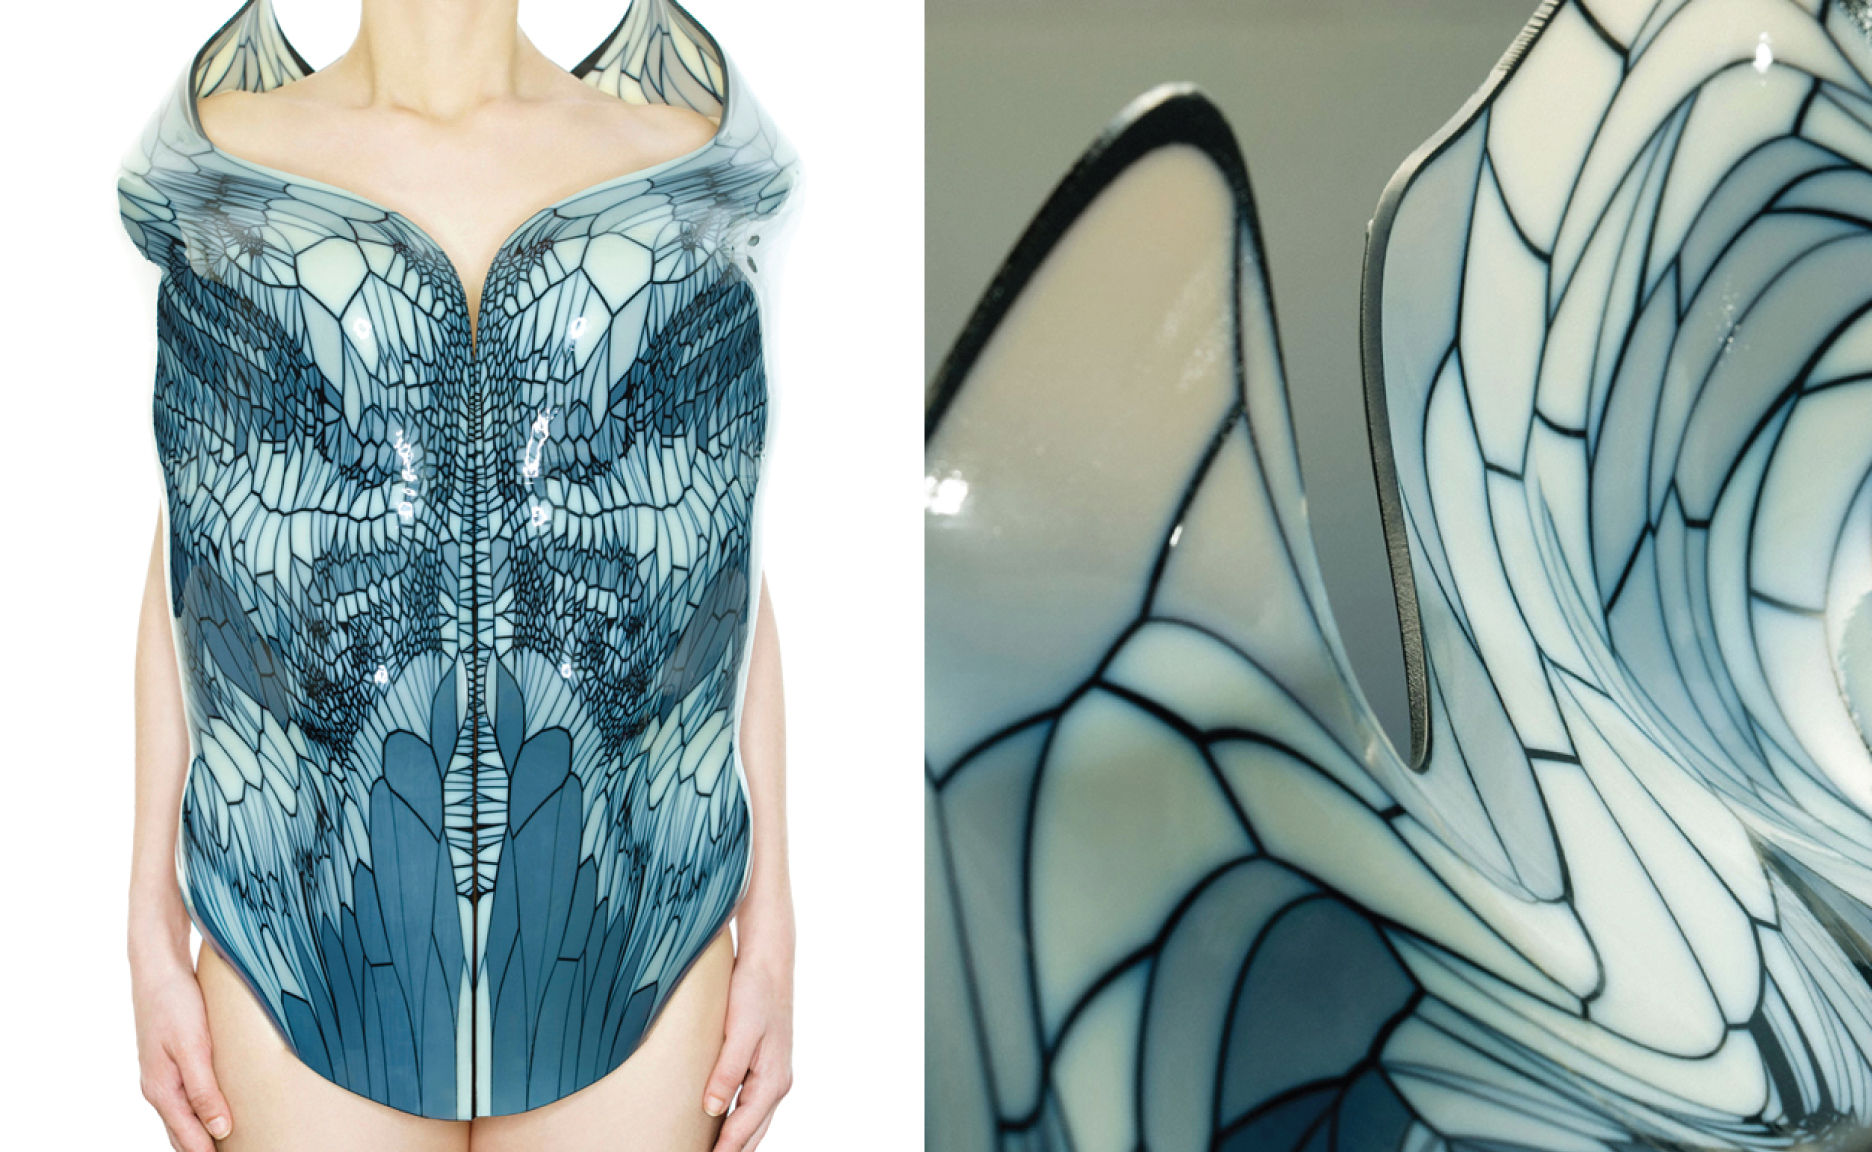
\includegraphics[width=\columnwidth]{images/arachne.jpg}
\caption{Arachn\`{E}Armor / Corset by Neri Oxman (2012), Digital Materials Centre Pompidou, Paris, France. The form of the web on the piece is determined by the anatomical location of a person's rib cage \cite{oxman_arachne}. }
\label{fig:arachne}
\end{figure}
\end{center}

\item \textbf{Documentation and remixing:} Computationally generated designs are generated by a program. This program can be shared with and modified by other designers, and can also serve as a form of documentation of the design process itself. 

\begin{center}
\begin{figure}[h!]
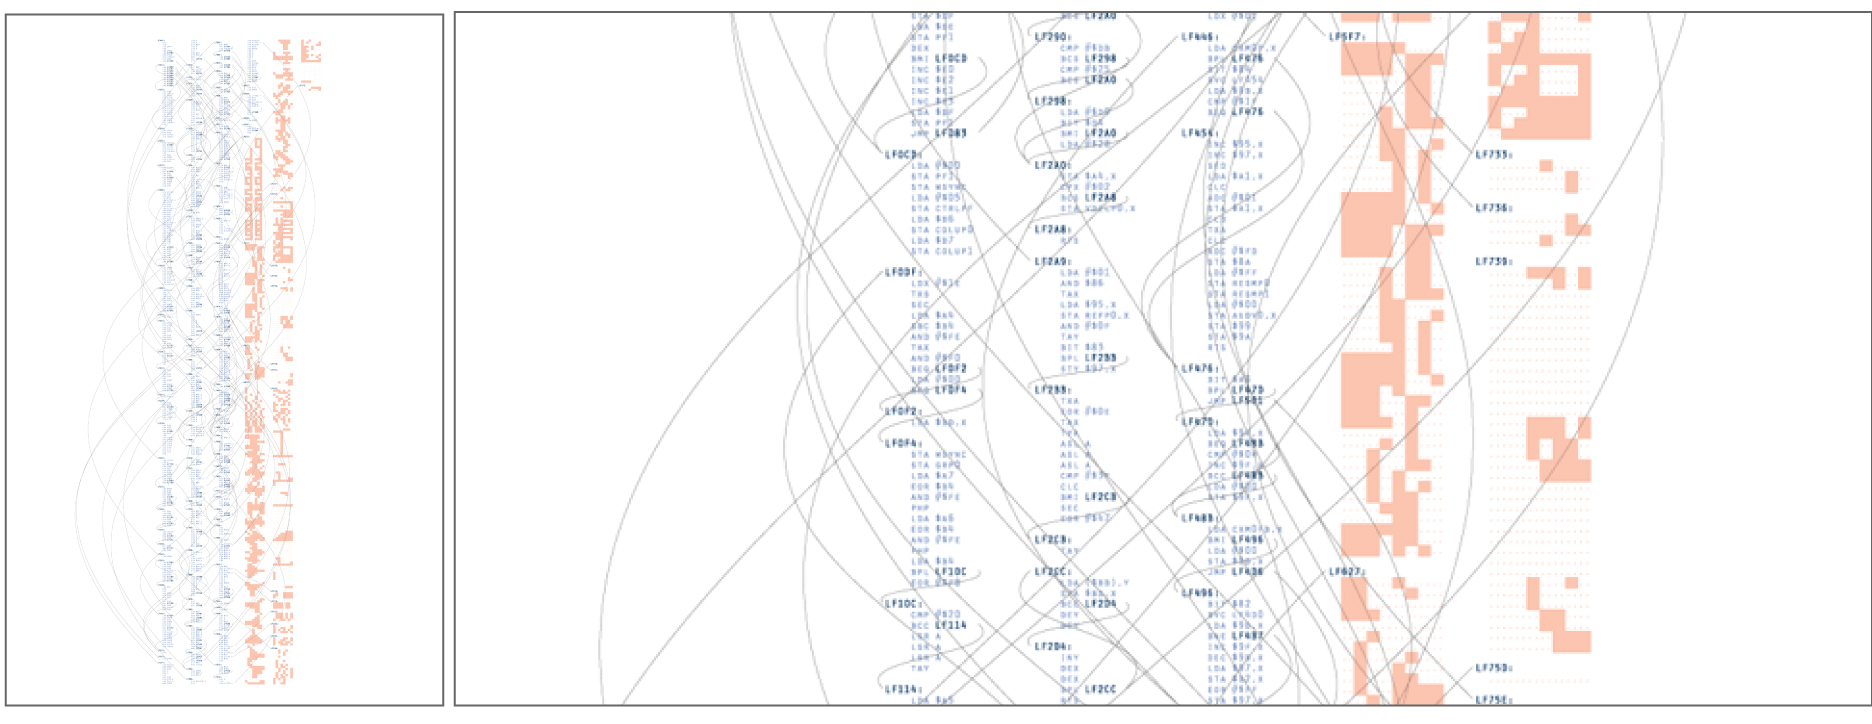
\includegraphics[width=\columnwidth]{images/distillamap.jpg}
\caption{Contra from Distellamap Series by Ben Fry (2005). Digital Print. The Distellamap series translates the code from a number of Atari2600 video games into a series of visualizations. Assembly code from each cartridge is shown in blue, with connection lines denoting ``go to" statements. Data are shown in orange \cite{fry_website}. }
\label{fig:arachne}
\end{figure}
\end{center}

\end{itemize}	

In combination with these affordances however, computational design also contains a number of unique challenges:
\begin{itemize}
\item \textbf{Formalizing complex problems} As design problems grow in complexity, formalizing the problem in a manner that can be expressed programmatically becomes challenging. Writing an algorithm to generate a single visual pattern is simple, however writing a program to incorporate that pattern into the design of a complex assembly is difficult. 
\item \textbf{Creating singularities:} A designer will often choose to deviate from a set pattern or structure at specific points in order to create a special emphasis in the area of deviation. Because computational design is governed by a systematized ruleset, the methods of breaking these rules at arbitrary points are often unclear or tedious to implement. 
\item \textbf{Selecting a final design:} The systematic approach to computational design gives the designer the ability to produce extremely large numbers of solutions to a single design problem. While this is useful in situations where multiple solutions are required, when a single design must be chosen, the process of deciding on a solution is often difficult and sometimes arbitrary, especially if the decision is based on aesthetic criteria.
\end{itemize}

\section{Digital Fabrication} Although computational design is performed on a computer, the artifacts generated by computational design are not restricted to the screen. Digital fabrication technology provides the opportunity to translate digital files to physical form. Digital Fabrication is supported through computer aided design (CAD) technology. CAD involves the use of a software tool to design an object. Some form of CAD file is generally required to control a computer numerical control (CNC) machine, enabling digital fabrication \cite{dunn}. Digital Fabrication is the process of using computer-controlled machines to fabricate objects specified by a digital tool path. Digital fabrication shares many of the affordances of computational design. In particular, it allows for the creation of physical objects with a high degree of complexity, without skill in craft or extensive manual labor. Digital fabrication also allows for the rapid production of small volumes of similar or identical objects. Also, because the artifacts produced through digital fabrication are derived from digital files, anyone with access to the file, and a similar fabrication machine can potentially create a copy of the object, or remix that object with others. 

There are two primary forms of digital-fabrication manufacturing, additive and subtractive. Subtractive processes machine a part by removing pieces from the original material and include tools like laser cutters, CNC milling machines and vinyl cutters. Additive processes create a part by incrementally adding successive layers of material. 3D printers are most commonly associated with additive manufacturing, however ink jet printers and CNC embroidery machines also fit this definition. Although advances in additive technology are occurring at a rapid pace, at this point the material options for 3D printing are limited. Most 3D printers can output objects in plastics, ceramic and metal composites \cite{dunn}. Low-end 3D printers are even more constrained, and can only print in ABS plastic. Additive manufacturing is also extremely expensive and often constrained to small build volumes.%\todo{reference wood printing 3D printers, other novel 3D printing techniques} 

%\todo{insert picture of 3D printed and subtractive pieces}

Unlike most 3D printing technology, subtractive processes can work with a wide range of materials \cite{dunn}. Laser cutters work well with materials such as wood, leather, paper and cloth (figure \ref{fig:materials}). Vinyl cutters can also be used on cloth, paper, in addition to adhesive vinyl. Milling machines can cut parts from plastic, foam, metal and wood. In specialized cases these machines can also be modified to function in an additive manner with custom attachments. An example is the adaptation of a 3-Axis ShopBot to function as a threading device to facilitate part of the construction of a Silk Pavilion, created by the Mediated Matter Group at  the Massachusetts Institute of Technology  \cite{pavilion}. Large-scale subtractive fabrication machines also make it possible to work at a larger scale than additive processes \cite{dunn}.

\begin{center}
\begin{figure}[h!]
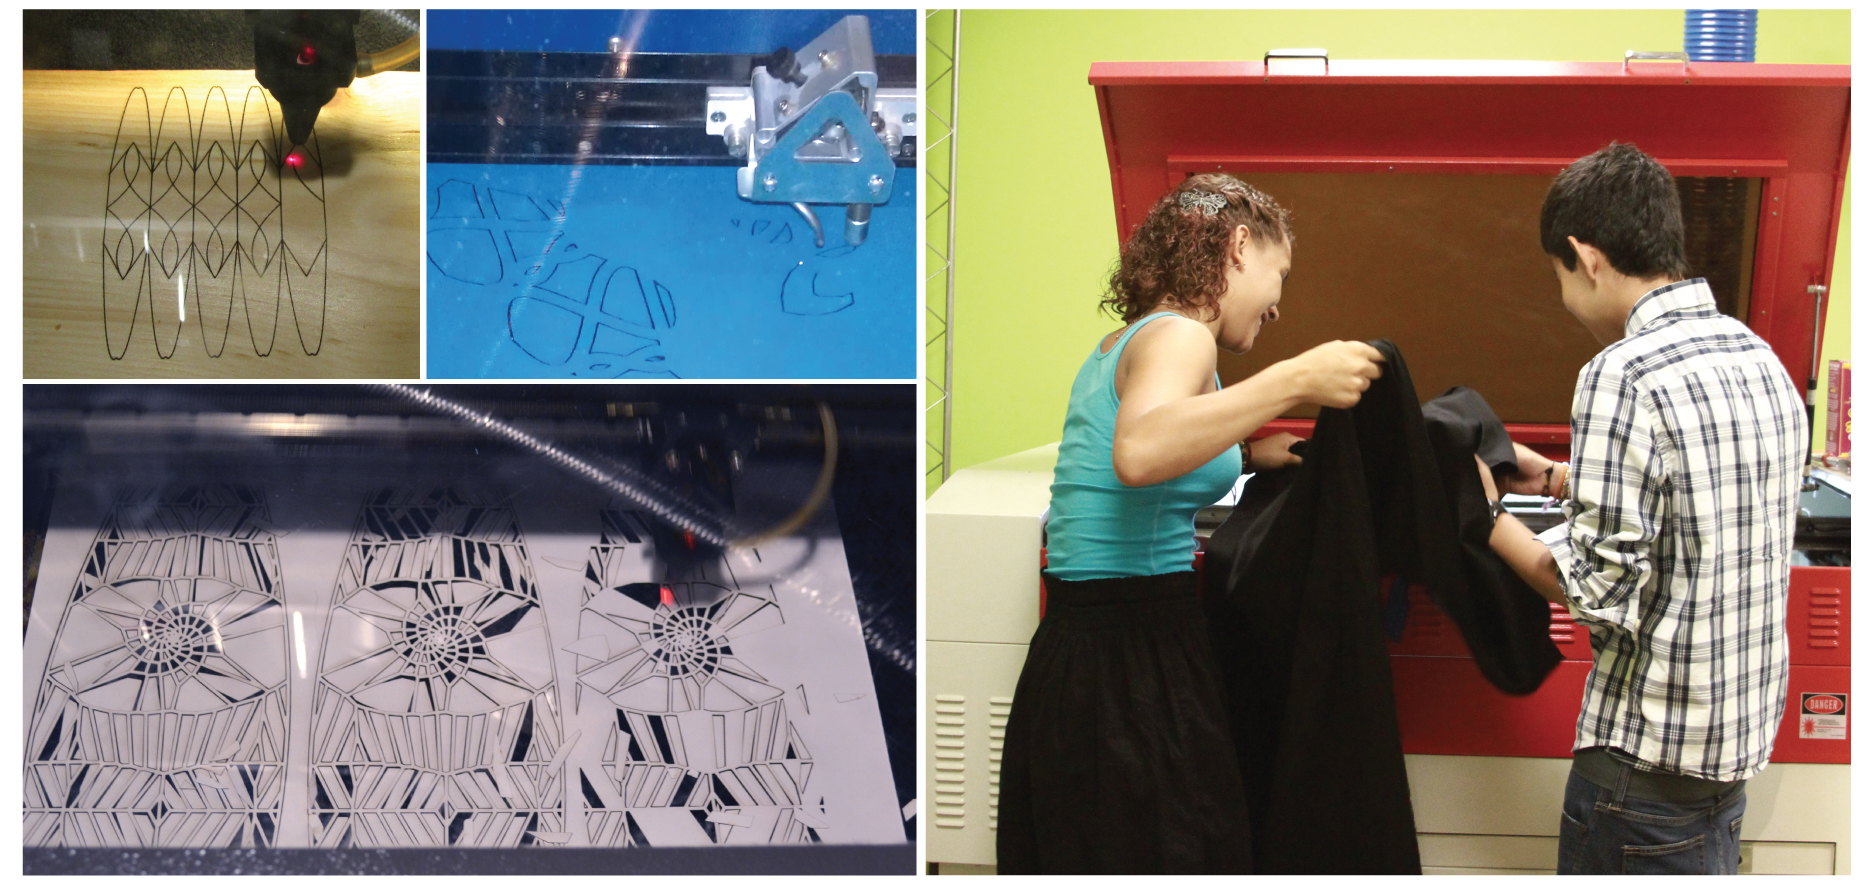
\includegraphics[width=\columnwidth]{images/laser_cutter_materials.jpg}
\caption{Various materials on the laser cutter. (Clockwise from top-left: laser-cut wood veneer, laser-cut fabric, loading fabric into the laser cutter directly from the bolt, laser-cut paper)}
\label{fig:materials}
\end{figure}
\end{center}

Widespread access to digital fabrication is growing. Digital fabrication machines are rapidly decreasing in price and increasing in availability \cite{gershenfeld}. This trend has allowed an increasing number of individuals and small groups to gain access to sophisticated manufacturing technologies, and signaled the growth of personal fabrication \cite{lipson}. Consumer 3D printers can now be purchased at prices ranging from \$1,000-\$3,500 dollars. Small scale laser cutters and milling machines are available at prices ranging from \$3,000 to \$5,000. In addition, other groups are producing open-source versions of commercial fabrication equipment, like the MTM Snap CNC-milling machine, the LaserSaur laser cutter and the RepRap 3D printer. Though these devices require additional levels of expertise to assemble, they point to to exciting future developments in affordable and open forms of digital fabrication. Machines like inkjet printers and craft CNC-vinyl cutters also function as personal fabrication devices and are extremely accessible and affordable. 

There also are options for individuals without direct ownership of a fabrication machine. Community hacker spaces like Artisans' Asylum in Cambridge Massachusetts, NYC resistor in New York, and Noisebridge in San Francisco, and organizations like the FabLab network provide access to shared digital fabrication facilities. Online services like Shapeways, Ponoko and SpoonFlower offer on-demand fabrication services to individual consumers for a variety of materials and machining processes. 

The rise of personal fabrication is often viewed as a component of the maker movement \cite{anderson}. The maker subculture is a technology-literate community that is engaged in the production of devices and artifacts in line with the do-it-yourself (DIY) philosophy. While maker culture has a strong technological focus, it also encompasses hobbyist craft techniques and materials. MakerFaire, one of the predominate maker culture events, showcases a range of DIY practice across science, engineering, art, and craft \cite{maker_faire}. Some of the primary tenants of the maker movement correspond to values frequently expressed in craft.

\section{Craft}
The cultural connotations of craft have varied throughout history. Once the primary means of producing functional objects, the role of craft changed following the industrial revolution. In the face of mechanized production, hand skills became less central to production, and design, traditionally unified with the role of the artisan emerged as a separate discipline \cite{abstracting_craft}. Despite the emergence of mass production, craft has endured, both as a recreational pursuit, and as set of valued artisanal practices. My personal interest in craft focuses on three specific qualities: materiality, pleasure and craftsmanship.
\begin{itemize}
\item \textbf{Materiality:} One primary aspect of craft involves the manipulation of physical materials \cite{on_craft}. Working with physical materials requires the use of one's hands, and is often an intuitive process. When we craft, we experience the feel of the paint brush moving across the canvas, the carving knife working through a piece of wood, a needle moving through cloth, or our fingertips pressing into clay. The decisions we make in the craft process are altered by the feel of working with the material. 

%\todo{insert picture of material evidence of craft (clay?)}

\item \textbf{Pleasure:} One of the responses to industrialism was the Arts and Crafts movement, initiated primarily by William Morris, and inspired by the writings of John Ruskin. 
The arts and crafts movement sought to restore the aesthetics and practices of traditional craftsmanship, in response to the negative aesthetic effects and working conditions of industrialism. Fundamental to the arts and crafts movement was the notion that the act of creating beautiful artifacts with one's hands was a pleasurable, essential human experience \cite{abstracting_craft}. This emphasis on pleasure is retained in conceptions of craft today.

\item \textbf{Unification of form and function:} Although not all craft is functional, many forms of traditional craft, including sewing, pottery, and carpentry can be applied the creation of useful objects. In addition to this functionality, craft often emphasizes the importance of beauty in the form and ornamentation of objects. Well crafted artifacts frequently demonstrate the successful unification of aesthetics and utility.\end{itemize}

%\todo{insert picture of decorative object from arts and craft movement}

\section{Algorithmic Craft}
Algorithmic craft is the combined use of computational design, digital fabrication, and hand craft. The merging of the properties of craft with computational design and digital fabrication allows for a creative practice that exhibits the variability and complexity of computation, the precision and repeatability of fabrication and the material, functional and aesthetic concerns of craft. Algorithmic crafting allows individuals to use programming and digital fabrication as a means of pleasurable and useful creative expression. In addition, algorithmic craft encourages the incorporation of the values of artisans and craftspeople in development of new methods of digital fabrication and computational-design tools, paving the way for new forms of innovation in these fields. Below I describe several examples of combined use of digital fabrication and craft, and computational design and craft ,respectively.

\subsection{Digital Fabrication and Craft}
Objects that emerge from a combined practice of digital fabrication and craft are often characterized by their physical craftsmanship, technical mastery and exceptional aesthetic. Practitioners in this space blur the boundaries between engineer, designer and artisan. One of the advantages of merging craft and digital fabrication is that it ensures that machine-produced artifacts retain their personal history. For his Hybrid Reassemblage pieces, Amit Zoran blended handcraft techniques like basket weaving and slip casting with 3D-printed forms  (figure: \ref{fig:hybrid}.) The process resulted in artifacts that retained the evidence of hand production in conjunction with forms made possible through digital fabrication \cite{zoran}.

\begin{center}
\begin{figure}[h!]
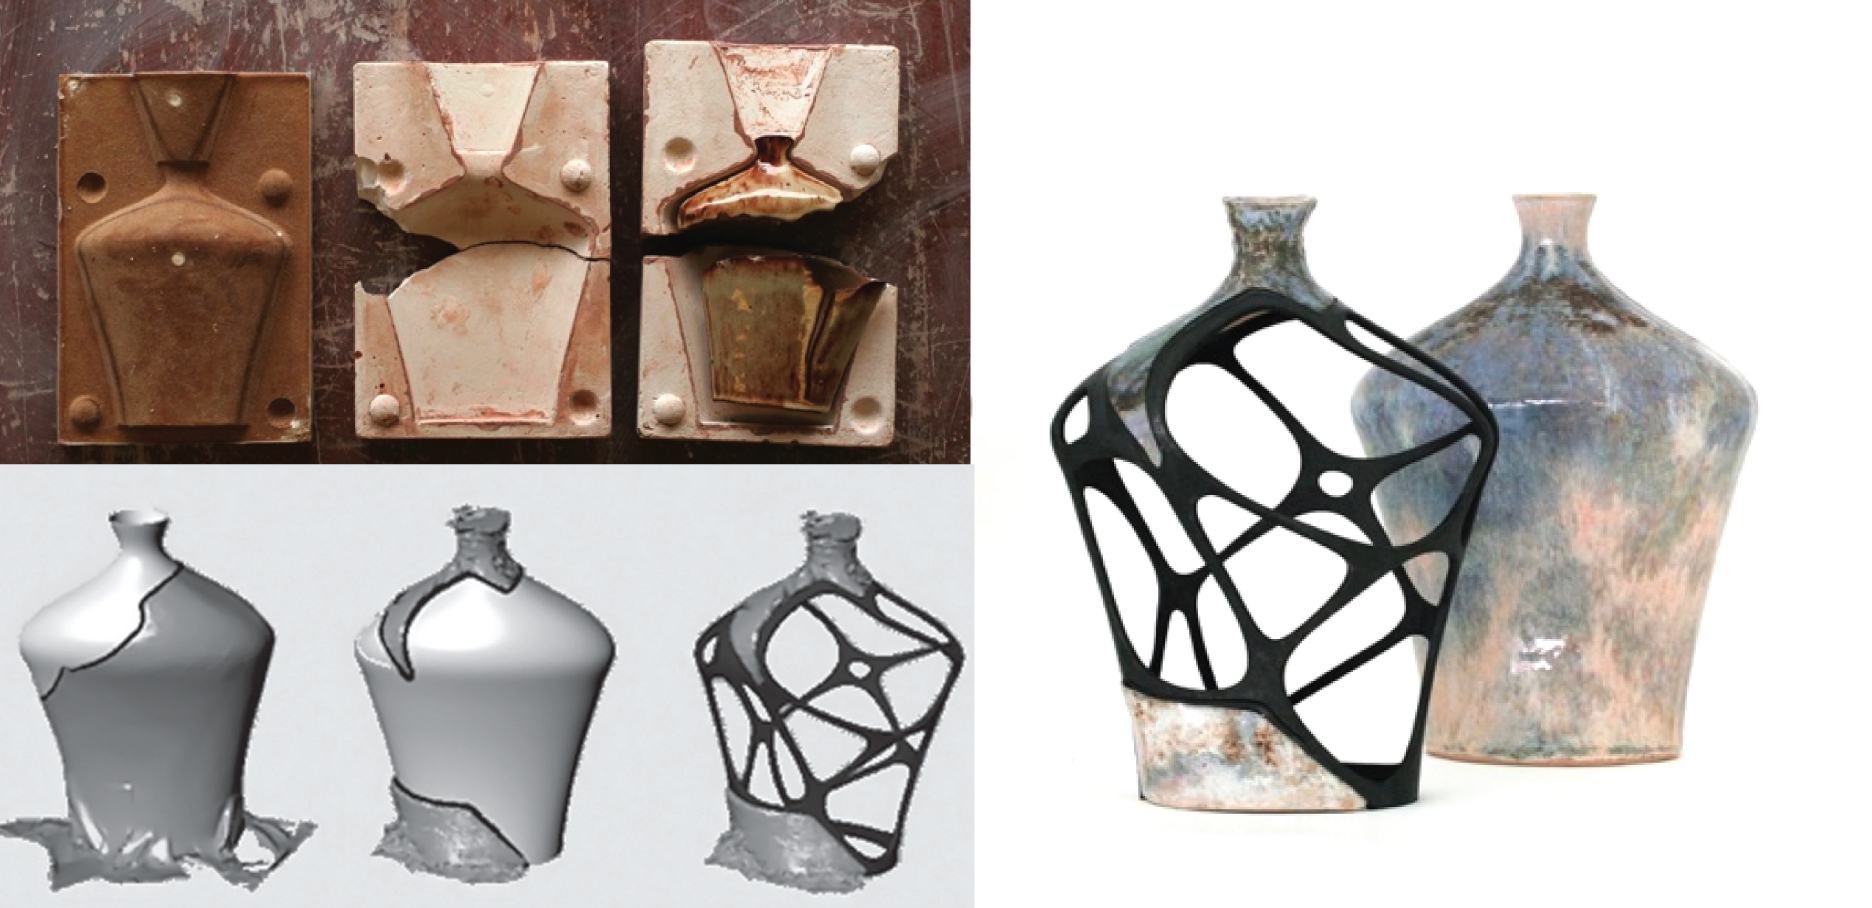
\includegraphics[width=\columnwidth]{images/amit.jpg}
\caption{A selection of vases from the Hybrid Reassemblage series by Amit Zoran (2010). Glazed
ceramic, SLS nylon element, epoxy glue and black spray paint.}
\label{fig:hybrid}
\end{figure}
\end{center}

Another advantage of combining digital fabrication and craft is that it affords openness and flexibility in the design of functional components. Peter Schmitt's plywood servo is a re-designed RC servo in laser-cut plywood. Although the parts of the servo are digitally designed, after fabrication the completed piece is constructed by hand. This process of hand construction gives the designer greater control in the form-factor and aesthetic of the servo, while maintaining its functional qualities \cite{plywood_punk}. As one sample application, the plywood servo was incorporated into a custom drawing machine called the Audiograph, producing a surprising and novel object with no precedent. The objective of the audio graph was to create a device with an appearance that was drastically different from customary home electronics and to explore people's reaction to the device in a home setting (figure: \ref{fig:plywood_servo})\cite{schmitt_thesis}. 

\begin{center}
\begin{figure}[h!]
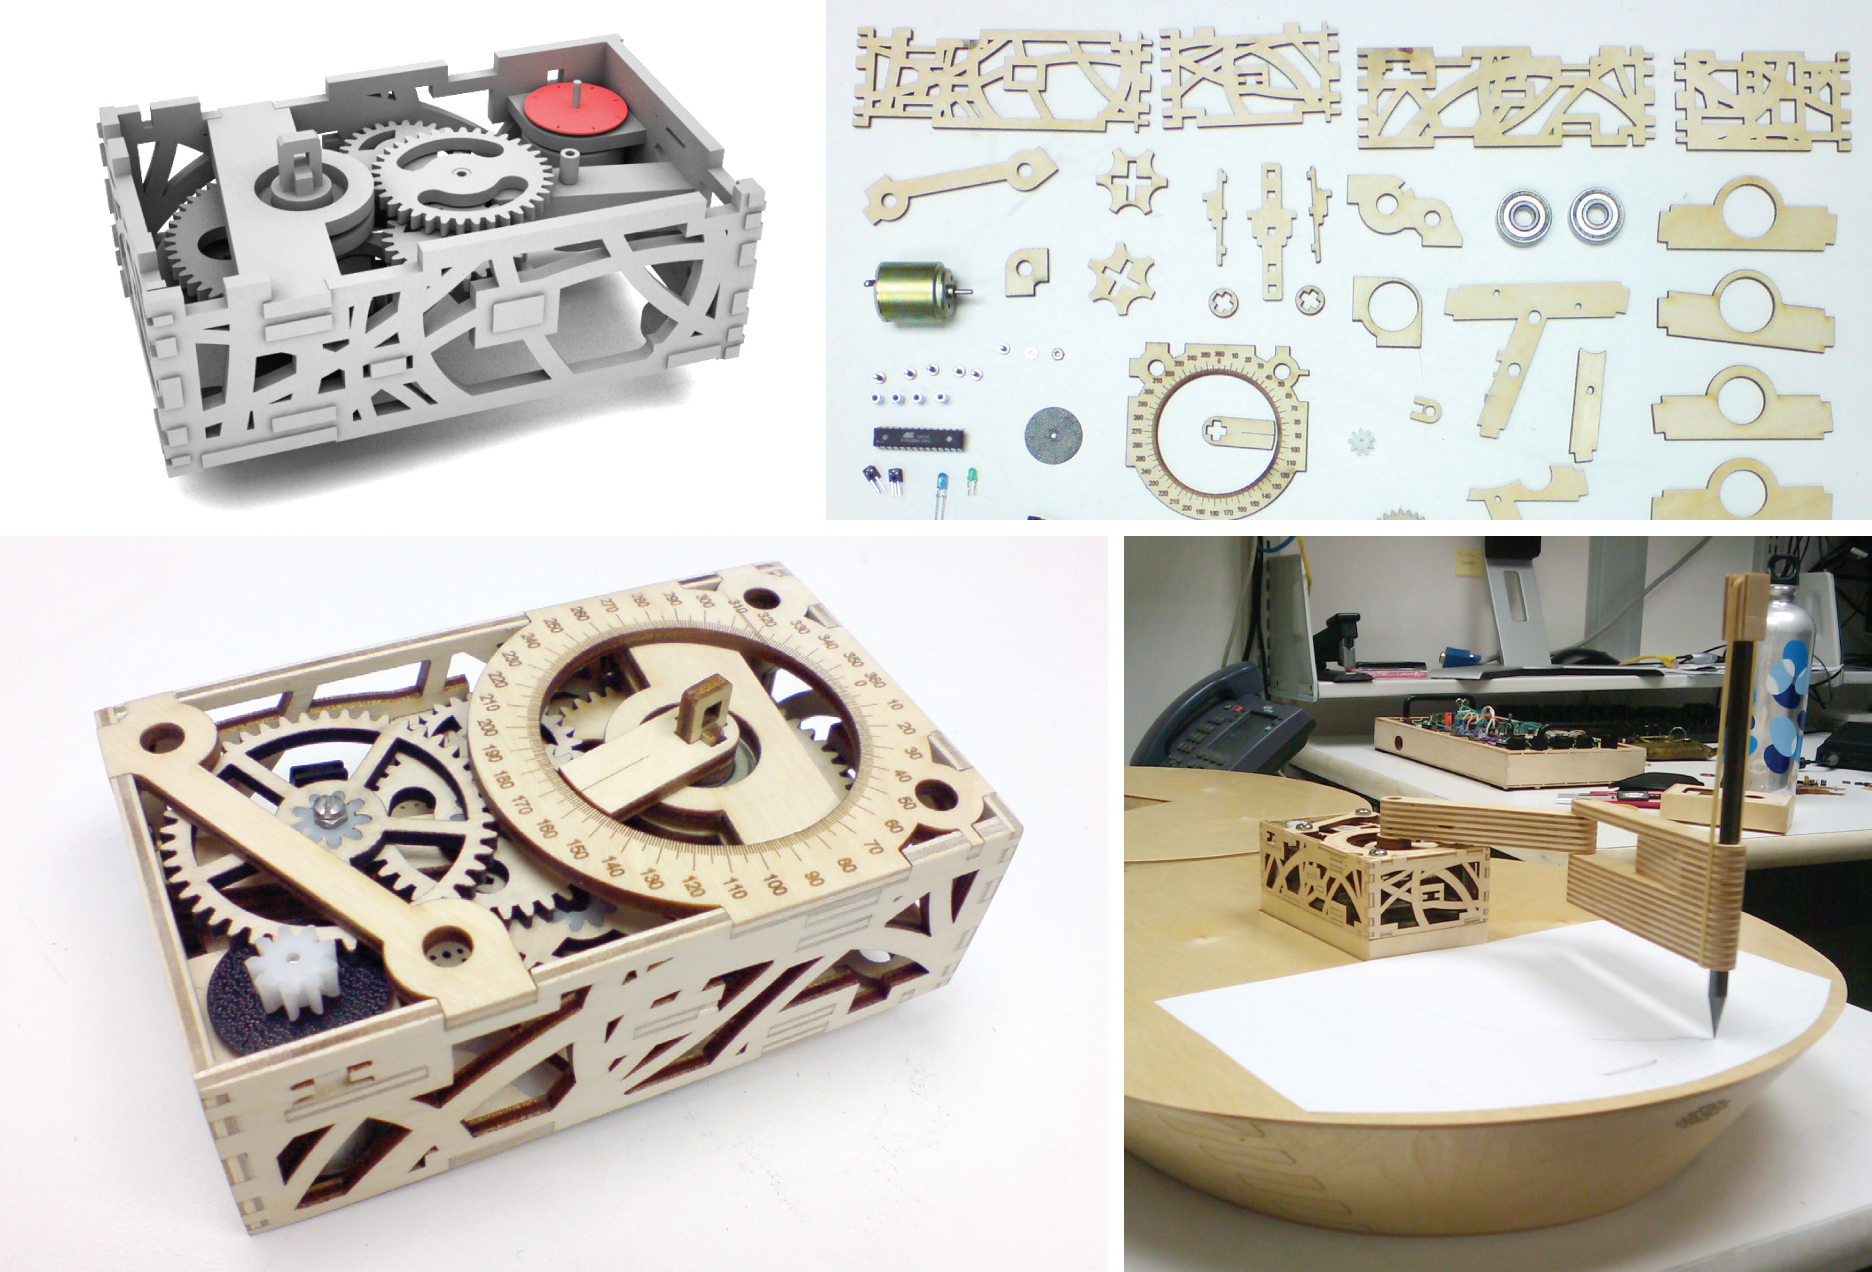
\includegraphics[width=\columnwidth]{images/plywood_servo.jpg}
\caption{Plywood Servo by Peter Schmitt (2011). (Clockwise from upper-left: 3D CAD model of partially constructed servo, laser-cut plywood parts and electronic components, Audiograph, completed servo.)}
\label{fig:plywood_servo}
\end{figure}
\end{center}

\subsection{Computational Design and Craft}
Similar to artifacts developed through digital fabrication and craft, the combination of computational design and craft also offers the opportunity to produce pieces that are connected to a distinct space, time and process, and that are shaped by material properties, while incorporating patterns and forms made possible through computational processes. The Random Number Multiple series was a project that produced screen prints from the work of computational designers and artists. Figure \ref{fig:thorpe_screenprint} shows a screen print translation of the computational artist Jer Thorpe's RGB-NYT word-frequency piece. The original piece was a digital image, which was generated from data describing the usage of the words ``red", ``green", and ``blue" in the New York Times between 1981 and 2011. In translating the digital piece to physical form the result is a distinct physical object, transformed by the material properties of screen printing. The artist describes the process on his website:

\begin{quotation}\textit{``This print turned out even better than I could have expected. The fine detail is amazing, the colours are rich and vivid, and the half-toning on the individual bars creates a jewel-like halo in the center that is fascinating to look at up close..This print was made with a semi-reflective ink, so it has a unique shimmer to it when viewed in the light."}
\end{quotation}

The rich material qualities Thorpe describes would be difficult to achieve by relying solely on a digital medium. In addition, Thorpe describes the pleasure he experienced in working with the tactile process of screen printing and how the experience provided important creative feedback for his computational work \cite{thorpe_website}. 

\begin{center}
\begin{figure}[h!]
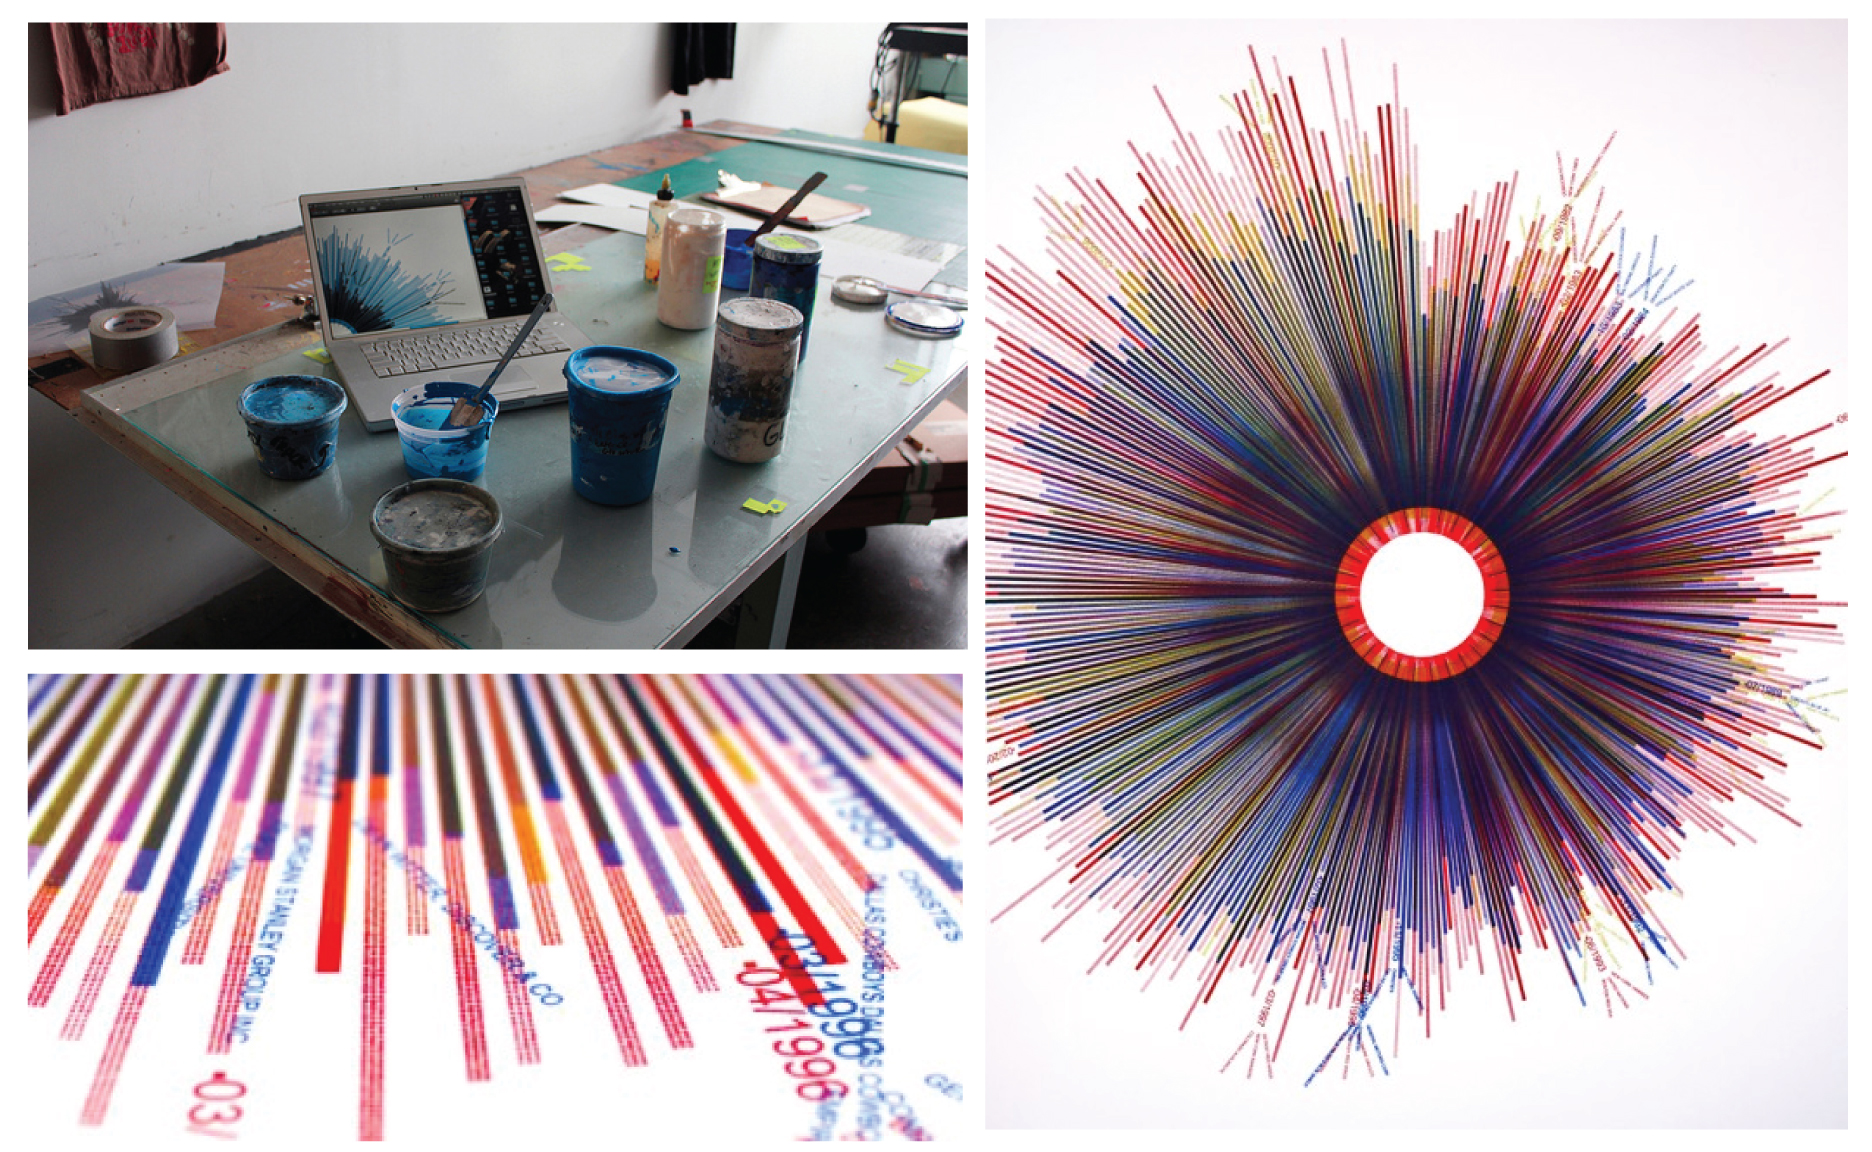
\includegraphics[width=\columnwidth]{images/thorpe_screenprint.jpg}
\caption{RGB � NYT Word Frequency by Jer Thorpe (2011). Part of the Random Number Multiples Series. Screen Print. (Counter-clockwise from upper-left: matching paint color to the digital image, close-up of print, complete print.)}
\label{fig:thorpe_screenprint}
\end{figure}
\end{center}
\vspace{-20pt}

Combining computational design and craft also offers the opportunity to engage craftspeople in the use of computational tools. The Processing Quilt (figure \ref{fig:processing_quilt}, was the result of a collaboration between Libs Elliott, a seamstress and quilt-maker, and Joshua Davis, a computational designer. Elliott created the quilt based on a Processing program created by Davis, which generated random triangle compositions. Elliott selected one specific composition and manually translated it to a grid, then cut out the necessary pieces, and crafted a completed quilt (figure: \ref{fig:processing_quilt})\cite{elliott_website1}. 

\begin{center}
\begin{figure}[h!]
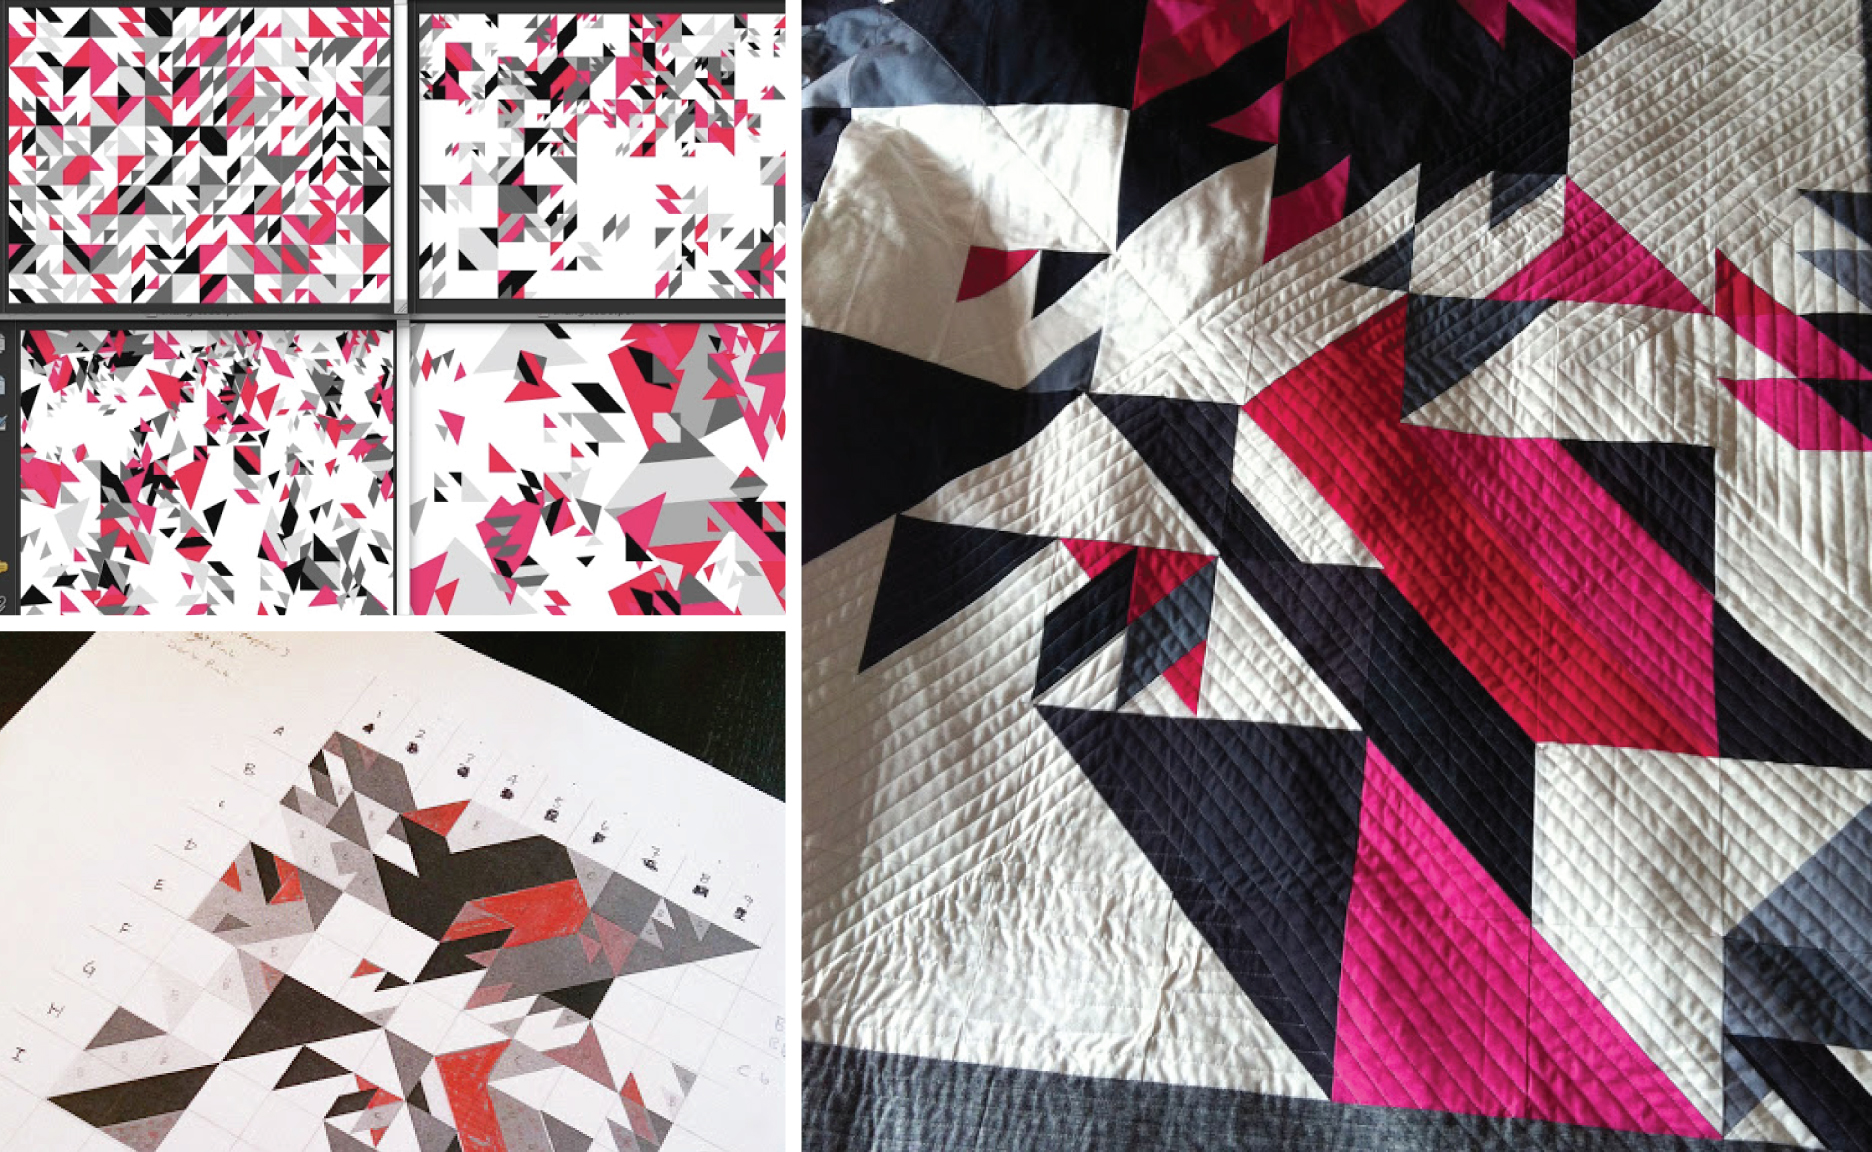
\includegraphics[width=\columnwidth]{images/processing_quilt.jpg}
\caption{Processing Quilt by Libs Elliott and Joshua Davis (2013). (Counter-clockwise from upper-left: auto-generated triangle compositions in Processing, hand-made quilt grid, finished quilt.)}
\label{fig:processing_quilt}
\end{figure}
\end{center}

The resulting artifact is a synthesis between computational aesthetics of the triangle composition and the texture created by the quilted pattern. The piece exhibits the skills and style of Elliott and the computational expertise and aesthetic of Davis. The transition between computational forms and craft processes can be a source of frustration however. On her website, Elliot remarked about the contrast between working with a computational tool and producing something by hand:

\begin{quotation}\textit{``I'm not going to lie--- quilting is a slow process and there's a certain level of frustration I have when I'm doing it. It's difficult to take something that works so quickly, like the Processing tool, to generate a hundred random compositions within an afternoon then force yourself to pick one image and slow it all down to an entirely manual process that takes days to produce \cite{elliott_website2}.}
\end{quotation}

Time is an important quality of crafting. Handcrafted artifacts often require a great deal of time to complete and involve repetitive tasks. Although frustrating for some, often, the longer it takes to create an object , the greater its value. Because the process of crafting is often pleasurable and contemplative, many people look forward to spending time productively engaged with their hands. In algorithmic craft, the role of digital fabrication is not to speed up craft, but to facilitate the translation of computational forms to physical materials. These physical forms in turn, can be shaped through craft processes, and imbue computational designs with individuality, utility and temporality. Several forms of digital fabrication machines are capable of producing forms that are suitable for both expert and novice levels of handcraft. Because subtractive fabrication technologies work with materials like wood, paper and fabric, they support the creation of objects that are readily shaped by the human hand. Laser-cut parts can be sanded, polished, painted, sewn or folded after they emerge from the machine. Vinyl cutters also can be used on cloth and paper. They also produce patterns in adhesive vinyl that can be applied to screens for for screen printing. Laser cutters and vinyl cutters also fabricate at a faster rate than 3D printers or milling machines, and permit a higher tolerance for error during the craft process because it is feasible to re-cut damaged parts.

\section{Challenges in Participation}
Through its association with hobbyist culture, many people consider certain forms craft to be accessible, and open to amateurs. Conversely, the combined use of computational design and digital fabrication is largely limited to experts and professionals. There are many practical barriers to novice participation in this domain. Most prominently, many of the programming languages used for computational design are difficult for novices to learn. In addition, a complex and convoluted process is required to translate a code-based design to a format that is compatible with fabrication machines \cite{gershenfeld}. Furthermore, the engineering challenges involved in designing complex objects from multiple digitally fabricated parts are extremely difficult to tackle for amateurs who are unfamiliar with CAD software. Although novice-oriented CAD software exists, most of this software does not support computational design. Similarly, most novice oriented programming environments cannot produce designs that are suitable for fabrication on their own. 

Significant perceptual barriers to participation also exist. Specifically, there persists among the general public a limited perception of the applications of programming. Many people consider programming to be irrelevant to their interests, and as a result, they lack motivation to pursue what they perceive to be a highly specialized and difficult undertaking \cite{resnick1}. There also are perceptions of digital fabrication which may hinder creative and open use of these tools. Personal-fabrication technology is often portrayed as a precursor to the production of replicator-like technology with the capacity to literally build anything, directly from atoms \cite{gershenfeld}. This view can act as a barrier to widespread engagement with existing forms of digital fabrication by setting up unreal expectations for this technology, or by portraying it as a variation on traditional forms of consumerism. The idea of fabrication as a perfect replication system also eliminates the need or desire for human engagement in the fabrication process, eliminating the entry points for craft. Daniella Rosner describes this view in her research:

\begin{quotation}
 \textit{A central element of these and other visions of the future is that craft is done for us: Kitchens tell us what and how to cook, eliminating the creativity and pleasure of cooking from scratch with what's on hand; object printers create flawless prototypes, eliminating messily glued-together chipboard and toothpicks. In this new world, craft becomes fetish---the proudly displayed collection of vinyl records shelved alongside an iPod and digital files \cite{rosner_craft_vs_design}.}
\end{quotation}

Algorithmic fabrication is an exceptional form of creation. Through the unification of computational design, digital fabrication and hand production, one can create functional, beautiful and unique objects. If we are to extend practice of algorithmic craft beyond people with formal training in computer science and computer-aided design, however, it is necessary to create accessible and open tools for programming and digital fabrication. These tools must be supported with practices that foster an understanding of the principles of computation, craft and digital fabrication and how they can work together for personal creative pursuits. 



%% This is an example first chapter.  You should put chapter/appendix that you
%% write into a separate file, and add a line \include{yourfilename} to
%% main.tex, where `yourfilename.tex' is the name of the chapter/appendix file.
%% You can process specific files by typing their names in at the 
%% \files=
%% prompt when you run the file main.tex through LaTeX.
\chapter{Related Software Tools and Research}
Computational design and digital fabrication are supported through the use of a variety of Computer Aided Design (CAD) software. There are six primary categories of existing software that are relevant to the study of the convergence of these fields: 

\begin{enumerate}
\item{programming tools for computational design.}
\item{Professional CAD tools with computational-design functionality.}
\item{Entry-level CAD tools.}
\item{Entry-level programming environments.}
\item{Novel fabrication and CAD tools.} 
\end{enumerate}

While some tools fall into several of these categories, it is useful to highlight the general functional distinctions and design strategies of each group of tools. 

\section{Programming tools for computational design}\label{programming_libraries}
Many of the examples of computational design referenced in section \ref{sec:computational_design} were created through the use of custom software tools written in a wide variety of programming languages, libraries and environments. Arguably, computational design can be performed with any programming language that has the capability to output some form of graphic data. In order to facilitate the process, some people have developed programming libraries and toolkits explicitly for computational design. Here I list some of the most prominently used tools in this space and describe their relation to digital fabrication. openFrameworks is a popular open source C++ toolkit developed by Theo Watson and Zach Lieberman that is designed to support a number of creative applications of programming. The toolkit contains wrappers for a variety of commonly used C++ libraries including OpenGL, GLEW, GLUT, libtess2 and cairo for graphics and Assimp for model loading, and facilitates a more immediate use of these libraries in conjunction. Although openFrameworks is frequently used to create interactive screen-based projects, several extensions have been developed which allow for the import and export of .STL model data, making it feasible to use the toolkit to design for digital fabrication \cite{openframeworks}. 

\begin{center}
\begin{figure}[h!]
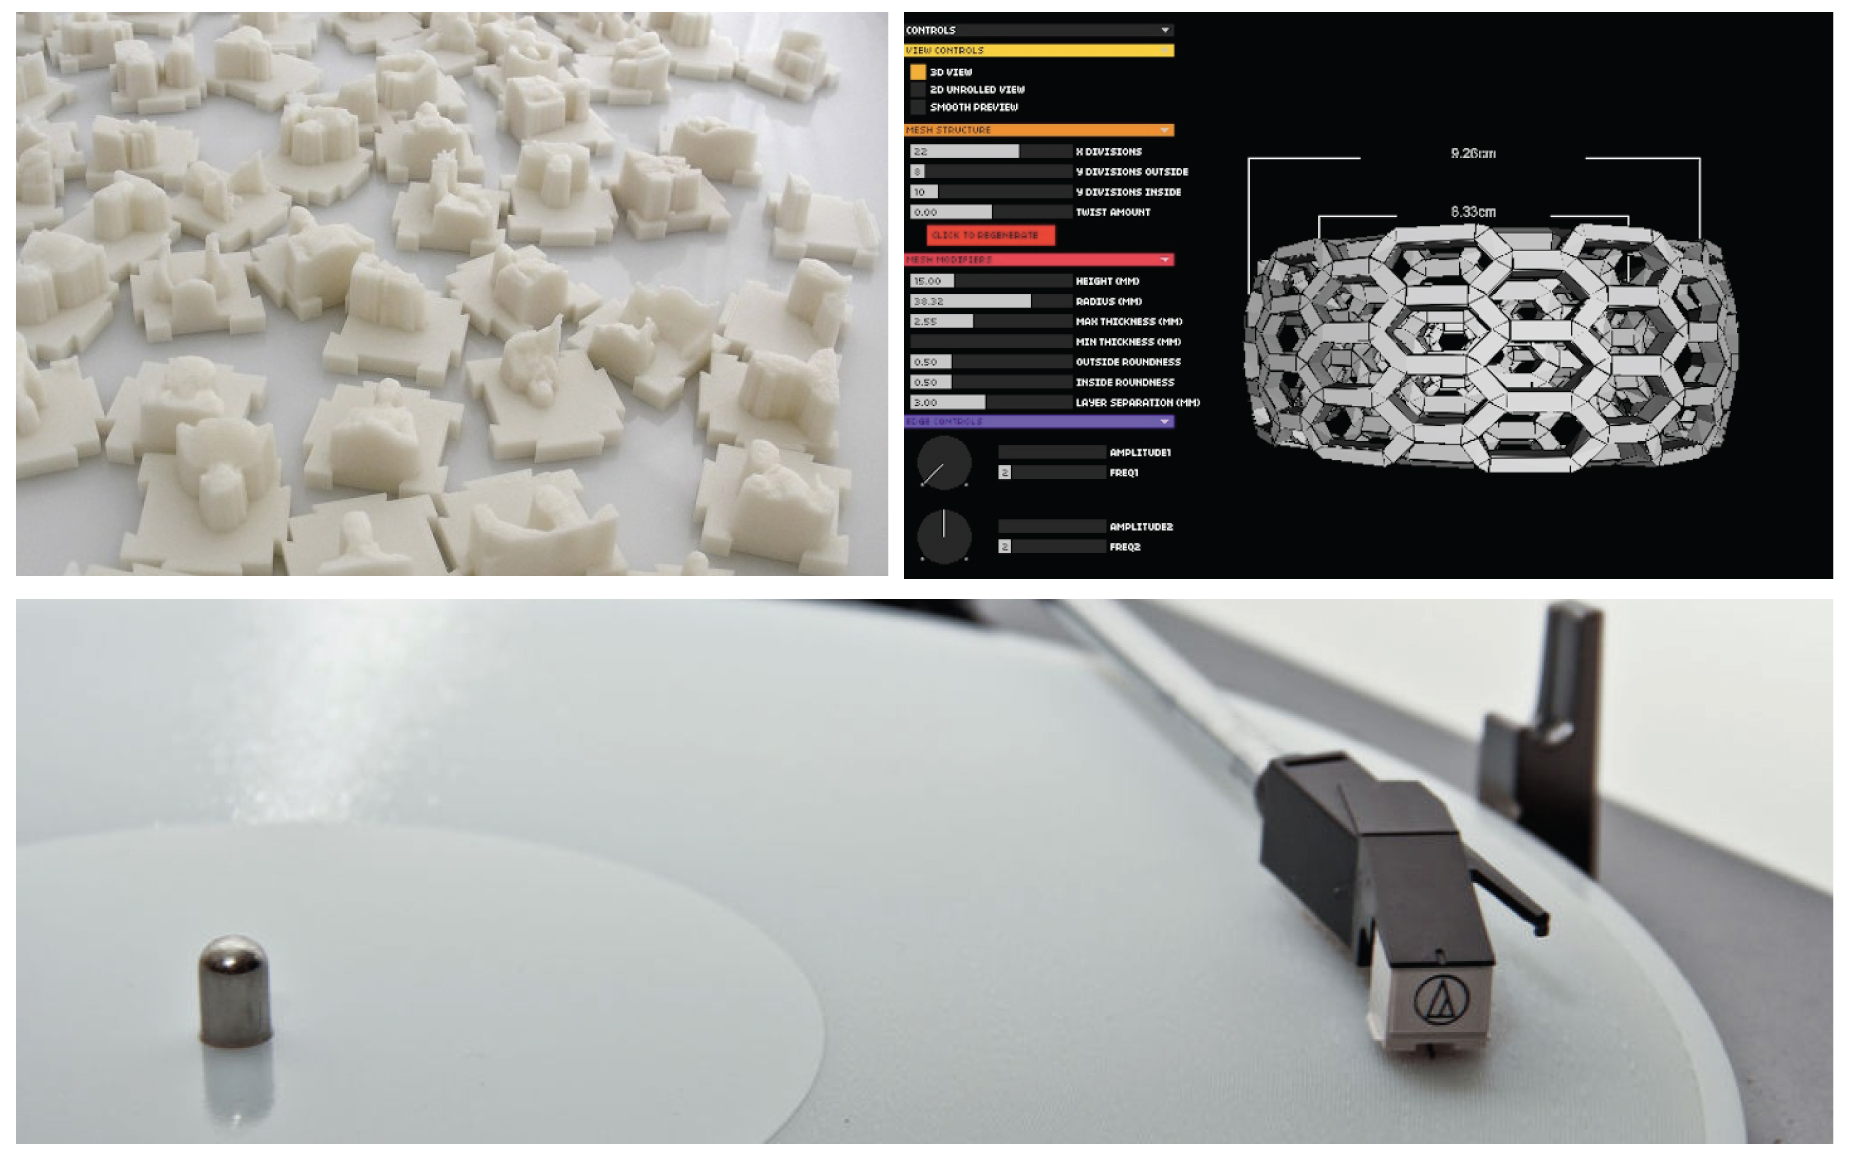
\includegraphics[width=\columnwidth]{images/framework_examples.jpg}
\caption{Clockwise from upper-left: Fabricate Yourself by  Karl D.D. Willis, 3d printed puzzle pieces featuring conference attendees (created with the openFrameworks toolkit, Kinect and a 3d printer), Cell Cycle Bracelet and Ring creation application by Nervous Systems (created with Cinder toolkit), 3d Printed functional record by Amanda Ghassaei, (created using Processing.)}
\label{fig:framework_examples}
\end{figure}
\end{center}
\vspace{-20pt}

Cinder is another C++ toolkit for computational graphics creation. Cinder was developed by the Barbarian Group, and requires greater programming expertise to use than openFrameworks \cite{cinder}. Similar to OpenFrameworks, Cinder is frequently used to create interactive installations, but it has been used for digital fabrication oriented projects. Nervous Systems used Cinder to develop their Cell Cycle iPad app, which creates cellular bracelets and rings for 3D printing \cite{cell_cycle}. 

Processing is a java-based programming language and development environment created by Casey Reas and Ben Fry. Processing is unique in that it is described as an entry level programming environment but is also an extremely successful professional computational-design tool. Processing contains several libraries that allow it to export to PDF and DXF formats, which enable a translation to digital fabrication \cite{processing}. 

All of these examples use textual programming as the sole means of design. In addition, because openFrameworks and Cinder exist as toolkits, they require the user to write programs in general purpose programming environments such as Visual Studio or Xcode. In the hands of experienced programmers, these tools facilitate remarkable forms of creative expression through code. Because of the difficulty of independently learning textual programming, it is uncommon for people without prior programming experience to use them for computational design without a great deal of instruction and support, let alone apply them to digital fabrication applications. Due to its unique positioning, Processing can act as an exception, something I discuss in greater greater detail in the section on entry-level programming environments.

\section{Professional CAD tools with computational-design functionality}\label{sec:professional_computational_design_tools}
Some professional CAD applications include functionality that makes it possible to use the software for computational design. Many popular graphic-user-interface (GUI) CAD applications include a feature that allows the user to automate certain elements of the program through scripting or programming. For example, in Adobe software like Photoshop and Illustrator, it is possible to write JavaScript-based programs to automate various application procedures. Similarly, 3D modeling tools such as Maya and Blender feature the ability to script behaviors in languages that are syntactically similar to Perl and Python respectively. In all of these examples the programming interface is omitted from the primary interfaces of the application, and must be deliberately activated by the user.

Some professional tools are more explicitly developed for computational design. One of the most prominent examples is Grasshopper, a third-party add-on for the Rhinoceros 3D modeling software. Grasshopper is a data-flow programming environment that lets users combine a variety of modules and blocks to create and adjust 3D models in Rhino. A textual coding module is also available and allows users to integrate C\# scripts using the Rhino API into their program.

DesignScript, a more recent computational design tool, developed by Autodesk, is a domain specific text-based programming environment and language that contains methods to generate and manipulate geometric models that are compatible with existing Autodesk applications. DesignScript is an add-on to the Autodesk AutoCad software and cannot be run independently. DesignScript is intended for use by experienced designers  and 3D modelers who posses a range of programming expertise. The language syntax is based on C\#, however it features the ability to operate in both associative and imperative paradigms, in an effort to support a pedagogical transition between basic and advanced levels of programming \cite{DesignScript}. 

\begin{center}
\begin{figure}[h!]
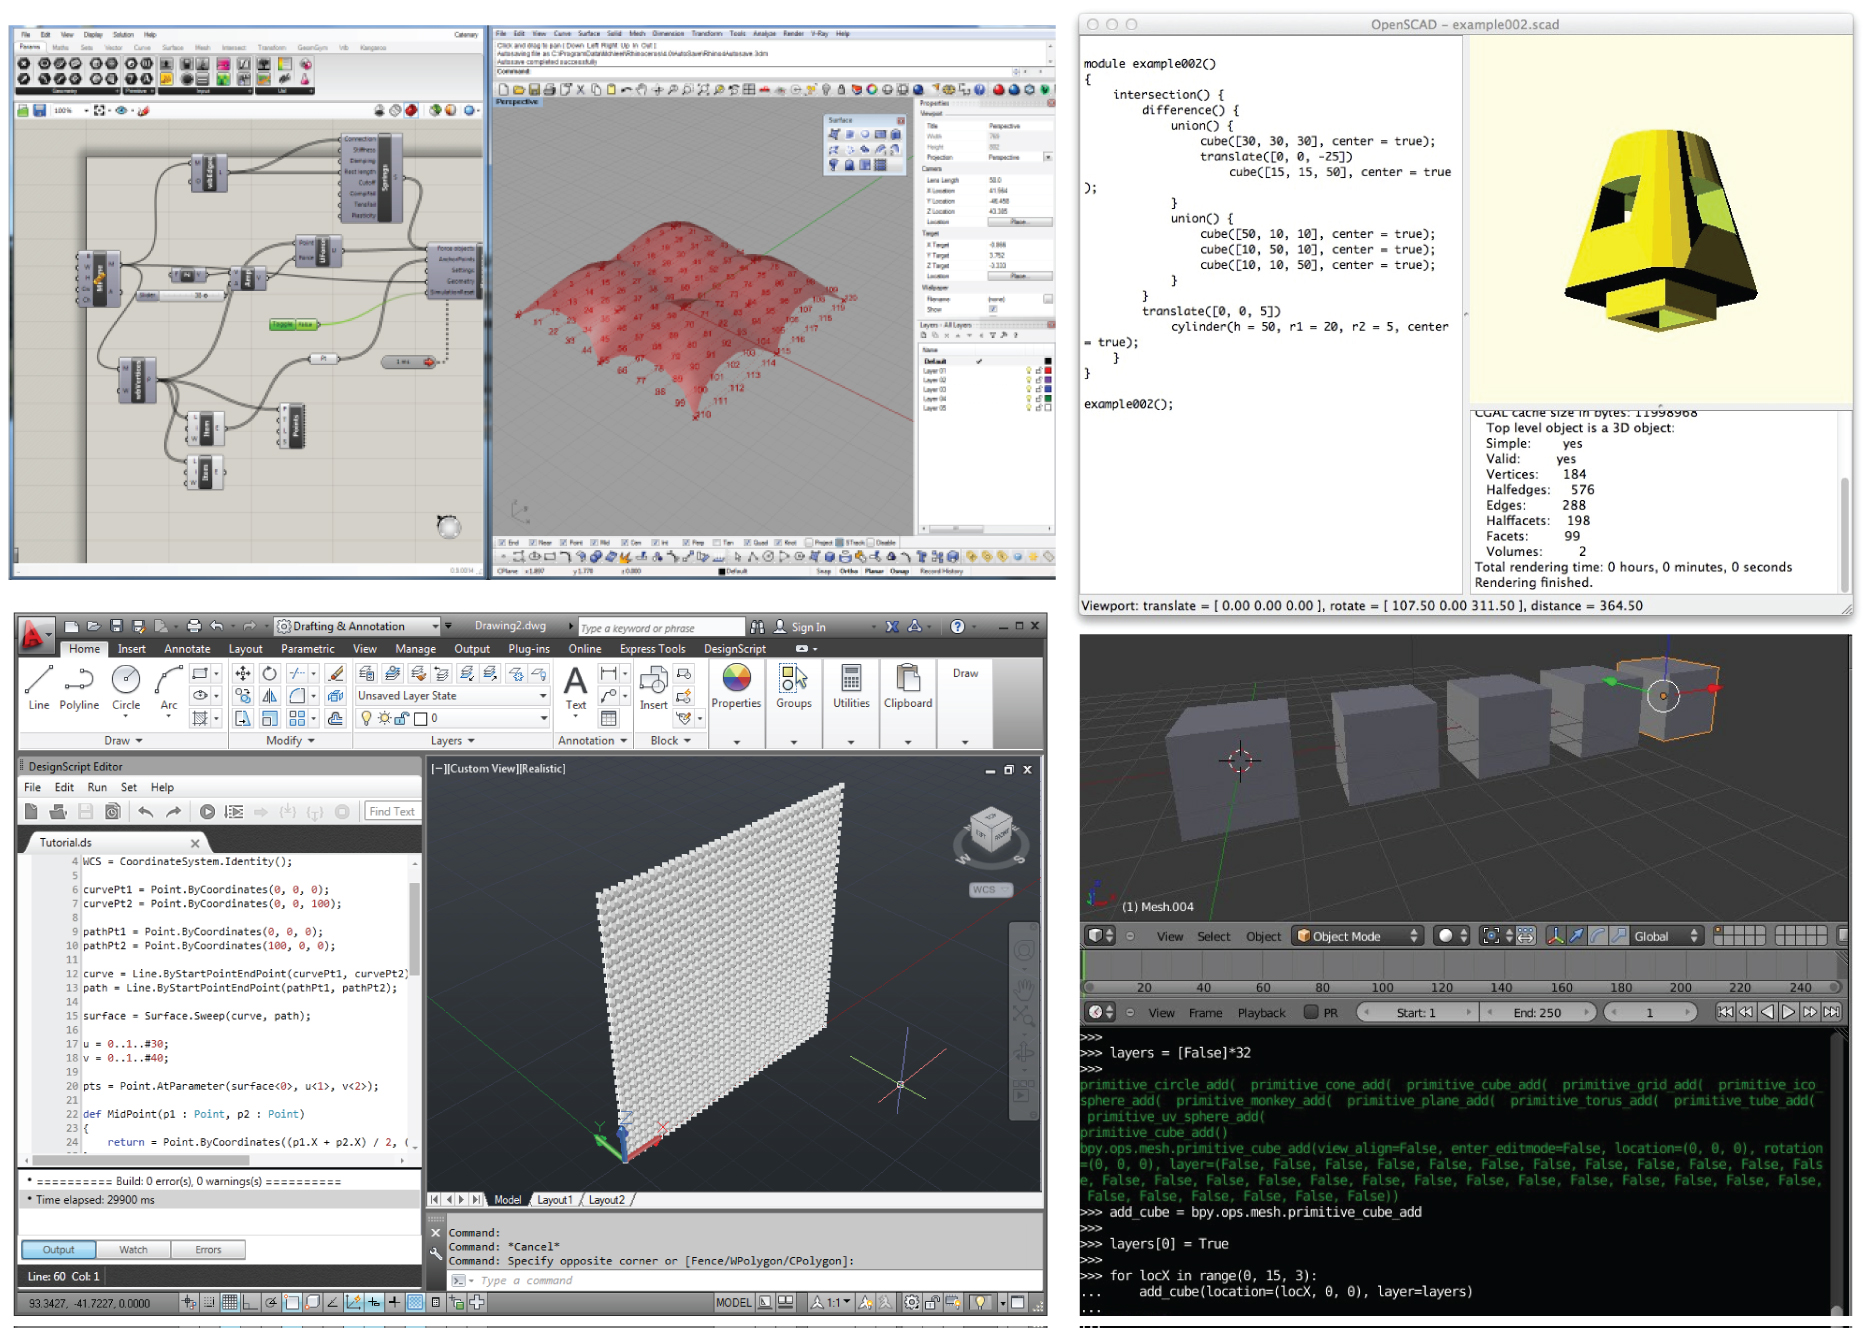
\includegraphics[width=\columnwidth]{images/cad_computation.jpg}
\caption{Computational design in professional tools. Clockwise from upper-left: A Grashopper program in Rhino, OpenSCAD, the Python scripting interface in Blender, DesignScript.}
\label{fig:cad_computation}
\end{figure}
\end{center}
\vspace{-20pt}

OpenSCAD is a script-based constructive solid geometry modeling tool developed specifically for CAD applications. OpenSCAD contains a custom programming language in which the user can create descriptions of 3d models in a textual format, and display them by compiling the script. This scripting behavior provides the user with pre�cise control over the modeling process and enables the creation of designs that are defined by configurable parameters, however this control comes at the cost of requiring the user to be familiar with textual programming and scripting. OpenSCAD is explicitly developed for experienced programmers and relies on textual input exclusively, In addition, unlike the prior tools mentioned, OpenSCAD is both free and open source, and several variations and derivatives of it exist \cite{OpenScad}.

One of the most important elements of these professional tools is their ability to import and export a wide variety of file formats, thus facilitating the transitions between a digital design and the required file type for a specific fabrication tool. Because to their high-cost and complex feature set, these professional tools are difficult to use without prior experience or extensive practice. With the exception of OpenSCAD, another defining feature of these tools is that they only available as plugins, add-ons  or are developed to supplement an existing graphical tool, rather than serve as the primary method of design. This status of programming as secondary form of interaction poses a practical barrier to novice use of the computational functionality of these tools; the scripting tools in illustrator and photoshop are difficult to locate, Grasshopper must be custom installed along with several dependencies, and only functions on Windows versions of Rhino, and Design Script requires the prior purchase of AutoCAD to operate. While these practical barriers can be overcome, their existence often prevents less experienced users from gaining access. More importantly, the positioning of computational functionality as secondary to the primary method of design points to a larger ideological classification of these forms of design as a specialized and exclusive, rather than serving as a primary method of design. 

\section{Entry-level CAD Tools}
A subset of CAD tools have been created that are designed to be more accessible to a wider range of people. These tools provide an option for individuals who lack the experience and access to professional level tools, however they also provide an opportunity for more casual participation in CAD. SketchUp is a 3d modeling tool developed by Google to enable easier forms of 3D modeling. Although SketchUp was not explicitly created to allow people to design for digital fabrication, several independently developed add ons exist that allow users to export designs to file formats that are compatible with a variety of fabrication machine \cite{sketchup}. TinkerCad is another 3d modeling tool designed for entry level users.  As opposed to SketchUp, TinkerCad is explicitly developed to assist in designing for 3d printers and has built in functionality to allow users to export their designs to the .stl format which is compatible with 3D printing \cite{tinkercad}. AutoDesk has also produced several entry level 3d-modeling applications as a part of their 123D series. Many of these applications are designed to interface with digital fabrication, including 123D Make which allows users to convert stock or uploaded 3d models into a series of flat parts which can be fabricated on 2-axis machines like laser cutters, and 123D Creature, which enables users to design a variety of creatures from a set of basic parts and then order a 3d printed model of their finished creature \cite{123D}.  AutoDesk Research has also developed MeshMixer, an application for the intuitive merging and manipulating high resolution triangle meshes. MeshMixer was released to the public and has since become a popular 3d design tool for hobbyist 3D printer users. 

\begin{center}
\begin{figure}[h!]
\includegraphics[width=\columnwidth]{images/novice_cad.jpg}
\caption{Entry-level CAD tools. Clockwise from upper-left: MeshMixer, 123D Make, TinkerCad.}
\label{fig:novice_computational_design}
\end{figure}
\end{center}
\vspace{-20pt}


All of the entry level tools listed above vary in their specific approach to creating more accessible forms of CAD. In general they feature a trade off between limited functionality and power, in favor of a simplified tool set and an easier learning curve. Despite these restrictions, it is possible to use these entry level tools to develop highly  complex and sophisticated models \todo{show example image of mesh mixer model}. A more pressing limitation of these tools is their ephemerality. Because entry level CAD tools are often free, and more frequently web based applications, it is common for them to suddenly become unavailable or no longer supported by the company that produces them. Tinkercad serves as a recent example of this wherein the parent company decided to transition to focusing on professional-level CAD tools and as a result, closed down the Tinkercad website and cut off access to the application. TinkerCad was recently acquired by AutoDesk and its website restored, however its future is uncertain.

Several of these entry-level tools also feature some form of scripting or programming functionality. A plugin for Sketchup allows users to automate certain actions by using the Ruby-based SketchUp API. TinkerCad allows users to create Shape Scripts, which are parametric models defined by javascript code. MeshMixer has an C++ API which is not yet publicly available, but is provided to interested parties upon request. While these computational features suggest compelling possibilities, similar to the professional level tools listed above, they are positioned as secondary ways of interacting, and are designed less deliberately than the primary features of the application.

\section{Entry-level programming environments}
Similar to entry level CAD tools, a number of wonderful applications have been created to introduce new programmers to the realm of computer science. 
Logo, a computational drawing program, serves as the seminal novice programming language founded on principles of constructionism and embodiment \cite{papert}. Logo allows users to  direct the movements of a virtual "turtle" with textual commands. The turtle can leave a trace of where it has been with a PENDOWN command, enabling users to write programs from an intrinsic perspective which produce geometric forms and patterns \cite{turtle_geometry}. The Scratch visual programming language is a notable successor to Logo, and allows users to create interactive projects by combining command blocks rather than writing textual code \cite{scratch}. Although Scratch is often used as a medium for interactive storytelling, it can also contains blocks that enable pen-up and pen-down functionality and can be used as a drawing tool similar to Logo. Turtle Art \cite{turtleart} and Design Blocks cite{design blocks} are two visual programming languages inspired by Logo that are designed specifically for visual composition.

\begin{center}
\begin{figure}[h!]
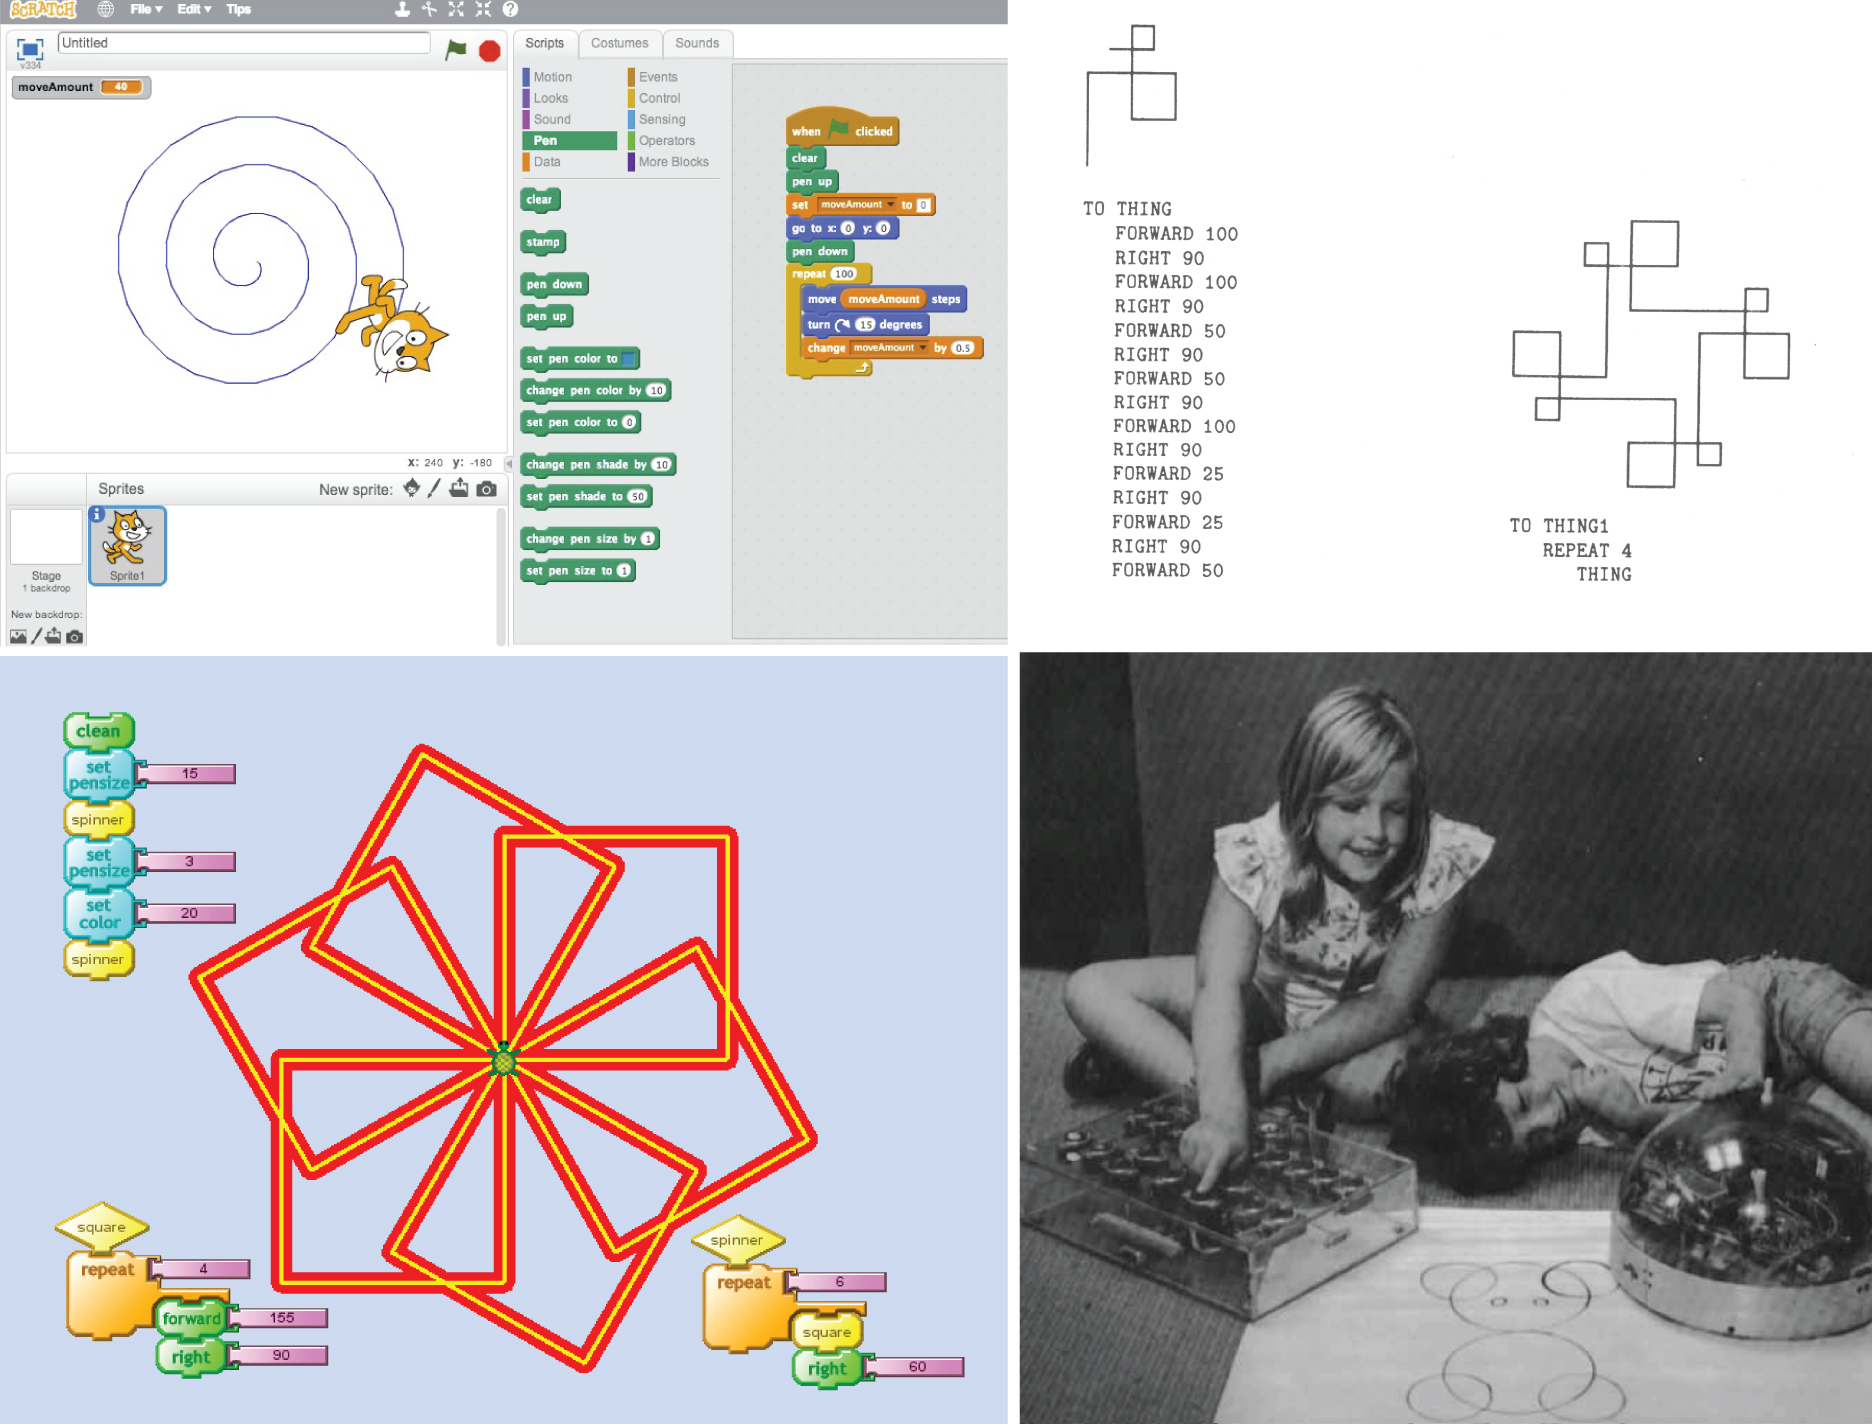
\includegraphics[width=\columnwidth]{images/novice_computational_design.jpg}
\caption{Entry-level forms of computational design. Clockwise from upper-left: A Scratch program using the pen tool, A design made in Logo by rotating a simple doodle, the Logo physical drawing robot, a sample Turtle Art program.}
\label{fig:novice_computational_design}
\end{figure}
\end{center}
\vspace{-20pt}

Logo, Scratch, Turtle Art and Design Blocks all support forms of computational drawing and, therefore, can be viewed as computational-design environments. There remains a gap, however, between novice-oriented programming environments and the novice-oriented CAD tools. In direct contrast to the novice oriented CAD tools described in the preceding section, although learning oriented programming tools can provide an excellent platform for generating digital computational design work, they often lack explicit features for generating and exporting designs that are compatible existing modes of digital fabrication. Although it is used by professionals, there have been many efforts to make Processing suitable for entry level programmers as well. The Processing drawing application programing interface (API) is simpler than other programing environments, and many instructional materials and example programs are provided on the processing website to support novice use. These features in conjunction with the processing libraries that enable the export of digital-fabrication-compatible file formats make Processing a more viable option for entry level computational design for digital fabrication. Despite this, Processing is not explicitly designed for digital fabrication. In practice it is difficult for new programmers to use it to design objects compatible with digital fabrication machines. If we wish to open this space for entry level practitioners, it is essential to design tools with computational design for fabrication as the primary function.

\section{Novel Fabrication and CAD tools}
In addition to these tools, there are a number of research projects involving novel forms of fabrication and software tools that demonstrate new approaches for computational design and digital fabrication. Sketch It, Make It is a 2D CAD tool that allows users to constrain their designs through gestures made using a digital drawing tablet \cite{sketchit}. Spatial Sketch is a tool that allows users to create abstract 3D sketches via their gestures, and then translates the sketches into a set of slices, which can be fabricated and combined into a finished piece \cite{spatialsketch}.  SketchChair allows users to design their own chair by sketching with a computer stylus \cite{sketchchair}. The resultant design can then be cut on a computer-numerical controlled (CNC) milling machine and assembled into a 3D object. SketchChair includes a simulation tool that allows users to test the usability of their chairs before they cut them. FlatCAD seeks to connect programming and digital fabrication and allows users to build customized construction kits with a laser cutter by programming in FlatLang, a novice-oriented programming language modeled on Logo \cite{flatcad}. Spirogator is a processing based tool that allows users to digitally customize a set of hypotrochoid geared-drawing tools and then view a simulation of those tools in action. The user then has the option of either exporting the resulting design generated by the digital gears and fabricating it directly, or exporting the file paths for the gears themselves, and fabricating them on a laser cutter, to be used as physical drawing tools \cite{spirogator}. 

\begin{center}
\begin{figure}[h!]
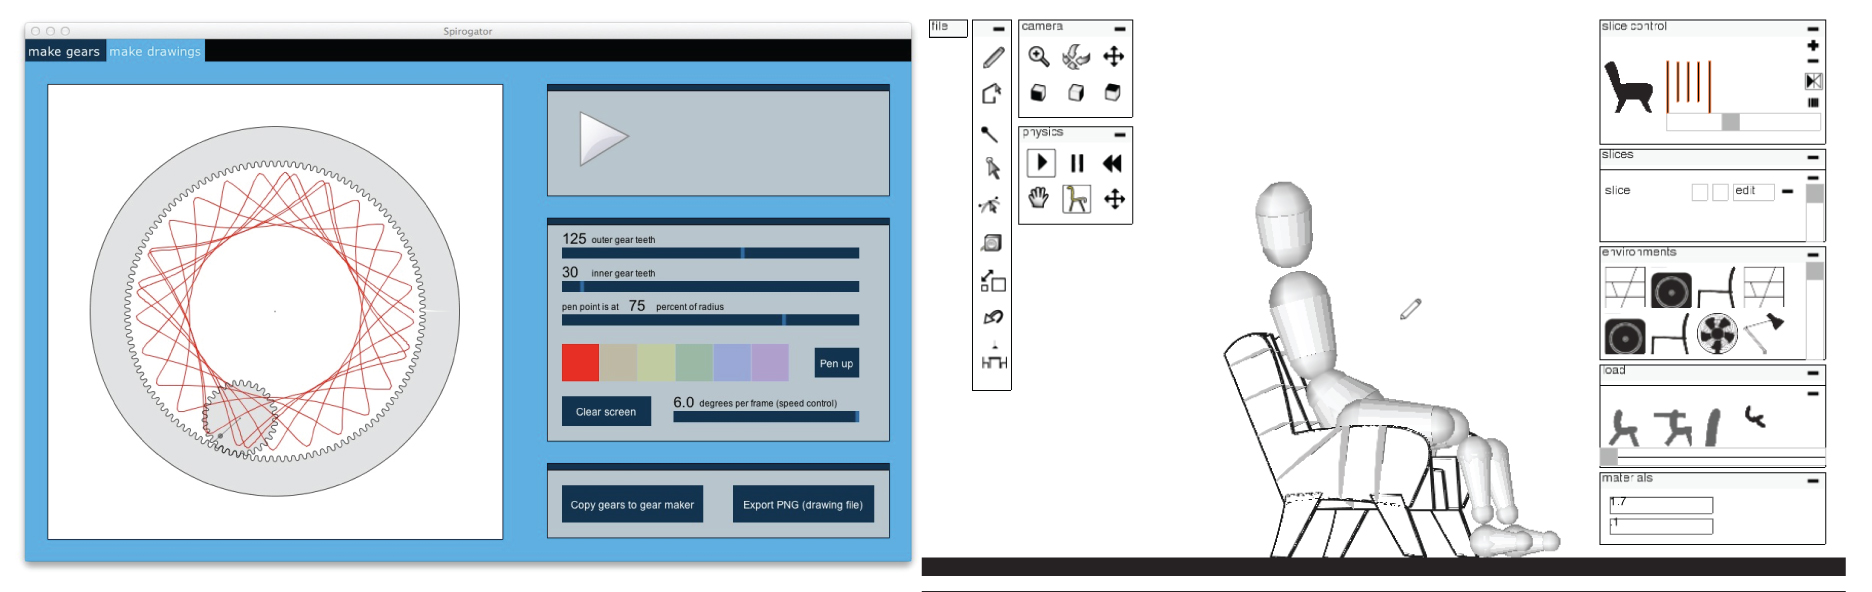
\includegraphics[width=\columnwidth]{images/novel_cad.jpg}
\caption{Novel CAD tools:  from left to right: Spirogator, SketchChair.}
\label{fig:novel_cad}
\end{figure}
\end{center}
\vspace{-20pt}


These examples share several important elements. They are restricted to a relatively narrow domain, but still support a wide range of design variations and personal expression. They contain intuitive and familiar methods of interaction often in the form of drawing and moving sliders. They contain explicit features for making the process of digital fabrication easier for new practitioners, and reduce the possibility of creating designs that will be infeasible to fabricate or are physically unstable. Spirogator and Sketch Chair's simulation tools are particularly interesting in this regard, as they assist the user in predicting some of the behavior of the resultant physical artifact prior to its fabrication. These qualities of domain-specificity, design flexibility, intuitive interaction and practical support for fabrication are important properties for any novice-oriented design software.

 \todo{images of novel cad tools}

%% This is an example first chapter.  You should put chapter/appendix that you
%% write into a separate file, and add a line \include{yourfilename} to
%% main.tex, where `yourfilename.tex' is the name of the chapter/appendix file.
%% You can process specific files by typing their names in at the 
%% \files=
%% prompt when you run the file main.tex through LaTeX.
\chapter{Objectives and Evaluation Criteria}
As indicated by the analysis of existing CAD and computational-design tools, many options exist to support novice entry into computer science and new tools are emerging that provide different ways of engaging in CAD and digital fabrication. At this point, few tools attempt to bridge accessible programing and novel forms of digital fabrication in relevant and engaging contexts for amateur programmers. Digital fabrication and computational design are two highly compatible domains with great creative potential. When combined with the values, practices, and aesthetics of craft, these shared practices offer new forms of expression and making. The objective of this thesis was to foster engagement in algorithmic craft by researching the relationship between programing, visual design, and physical construction. I conducted this research through the development of software tools that emphasized computation by positioning programing as the primary method of generating and manipulating designs. In doing so I attempted to retain a high degree of accessibility and intelligibility for new programmers, and a smooth transition from code to fabrication. Within this objective, I generated a set of evaluation criteria for prospective algorithmic crafting software. A successful tool should produce the following results:
\begin{itemize}

\item \textbf{Allow users to successfully create physical artifacts:} The artifacts themselves should be durable and useful.
\item \textbf{Afford a wide degree of variation in design and expression:} The personal aesthetic preferences of the creator should be apparent in the resultant artifact.
\item \textbf{Enable people to understand the functionality and utility of the programs they write:} Individuals should emerge from the process with a general understanding of some of the key components of computer programing, with an ability to articulate how these components function in their design. 
\item \textbf{Allow users to create objects and designs they would have difficulty generating with conventional techniques:} The tool should support the affordances of computational design, specifically precision, visual complexity, generativity and stylistic abstraction, as well as enabling people to take advantages of the properties of digital fabrication including  manufacturing speed, precision, and physical complexity. 
\item \textbf{Engender in users a positive, enjoyable experience:} Use of the tool and subsequent crafting activities should be pleasurable and intellectually engaging.
\item \textbf{Foster a sense of confidence:} After working with the tool, people should have increased confidence in their ability to successfully program, design, and use digital-fabrication tools. 
\end{itemize}

\section{Design Tools and Evaluation Methodology}
Over the course of my thesis, I developed and tested three software tools to support algorithmic craft. Codeable Objects is a domain-specific programing library for the design and production of lamps. Soft Objects is an expanded version of Codeable Objects intended primarily for computational fashion design. DressCode is a general-purpose integrated programing and visual design environment. Each tool was evaluated during one or more workshops with designers, artists, programmers or young students. I  documented each workshop through pre and post surveys, interviews, and photographs of student projects.  The surveys were aimed at understanding participant's previous experience in craft, programming and design, their interest in and attitudes toward craft, digital fabrication, and computation (before and after the workshops), and their engagement in and enjoyment of the workshops.

Surveys were administered at the start of the workshops and focused on participants� previous experience and attitudes. People were asked to describe their opinions about how programing and craft could be combined, and how they felt programming could extend or limit creativity. Surveys were administered again at the termination of the workshops and contained attitudinal questions that were matched to the pre surveys. In addition, post surveys contained a range of written questions asking the participants to describe their opinion of the success of their projects and their experience using Codeable Objects, Soft Objects or DressCode respectively.  

Individual interviews were conducted with the participants in the Soft Objects workshop, and the DressCode workshop. These interviews lasted an average of 15-30 minutes and were audio recorded and transcribed. During the interviews, the participants were asked to describe their experience in the workshop and talk about the process of conceptualizing, designing and producing their artifacts. They were asked to describe what they enjoyed, what was difficult for them, and what they felt they had learned through this process. Responses from the survey and verbal interview were then analyzed with project outcomes to determine if the essential qualities outlined in the evaluation criteria were achieved.  We also used this information to identify recurring and prominent themes in participants� experiences. In the following  three chapters, I detail the development, feature set, and evaluation of each design tool.
%% This is an example first chapter.  You should put chapter/appendix that you
%% write into a separate file, and add a line \include{yourfilename} to
%% main.tex, where `yourfilename.tex' is the name of the chapter/appendix file.
%% You can process specific files by typing their names in at the 
%% \files=
%% prompt when you run the file main.tex through LaTeX.
\chapter{Codeable Objects}

\begin{center}
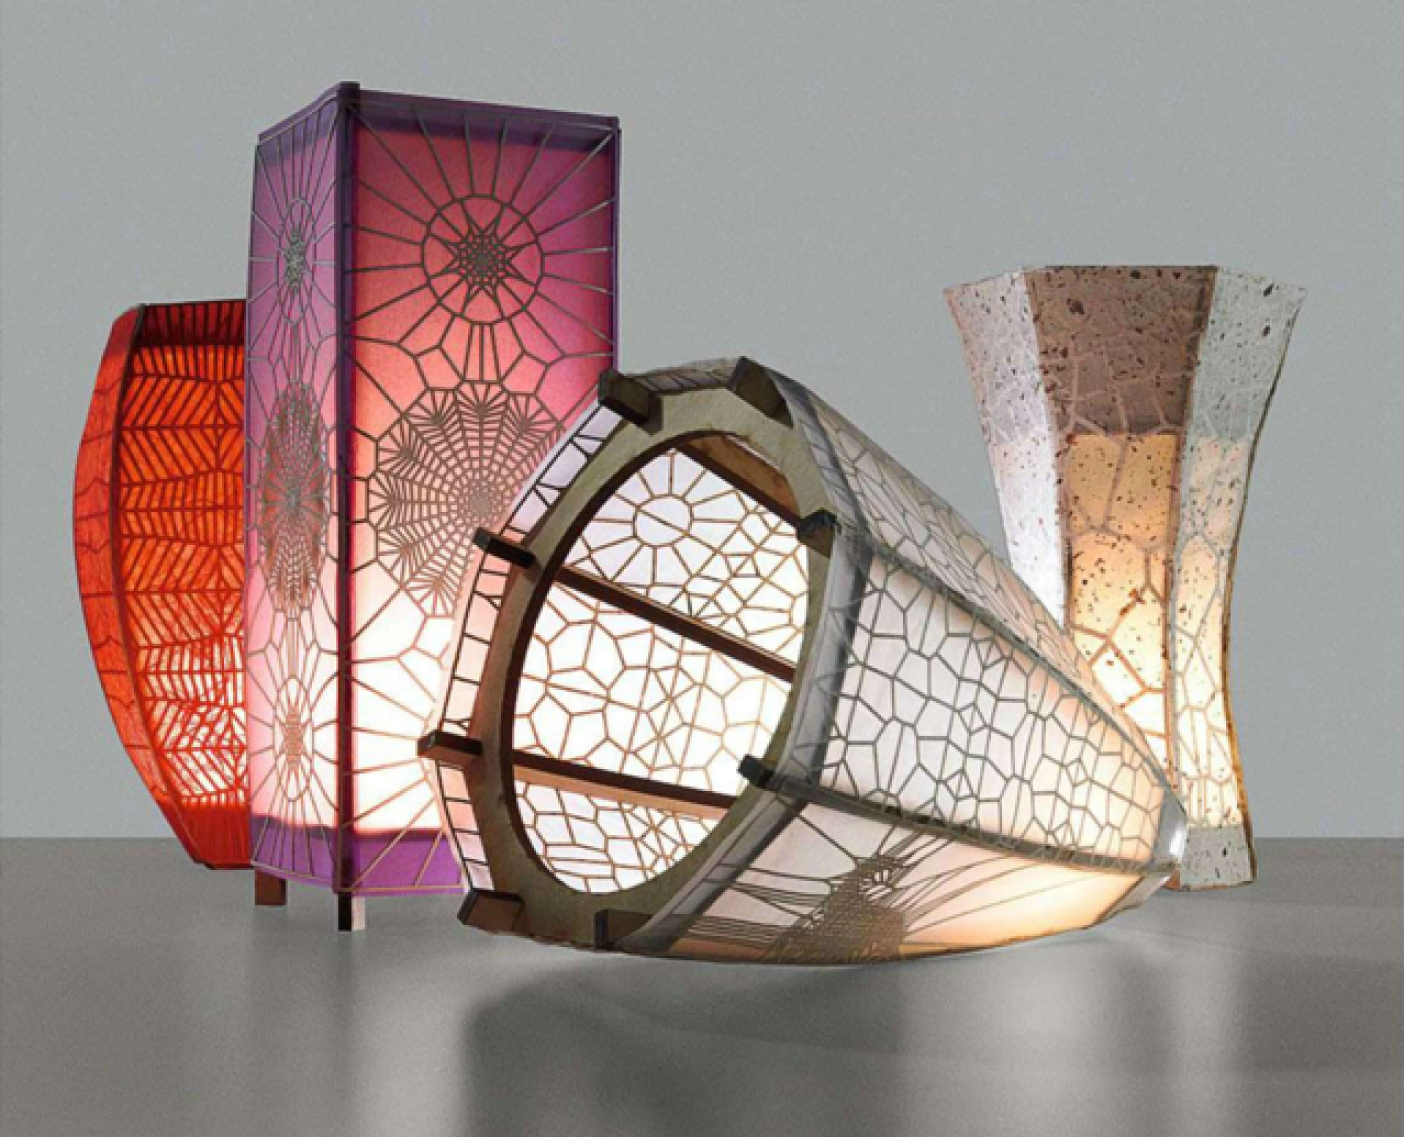
\includegraphics[width=6.5in]{images/finished_lamps.png}
\end{center}

Codeable Objects is computational design tool that allows people to design and export the toolpaths for a laser cut lamp. Because lamps possess an established function, but can vary immensely in their form-factor, the domain of lamp design offers a wide set of design possibilities for a concrete and useful end product. By introducing lamp design in the context of algorithmic craft, my goal was to allow people to construct unique lamps comprised of computationally generated forms and patterns. 
\begin{center}
\begin{figure}[h!]
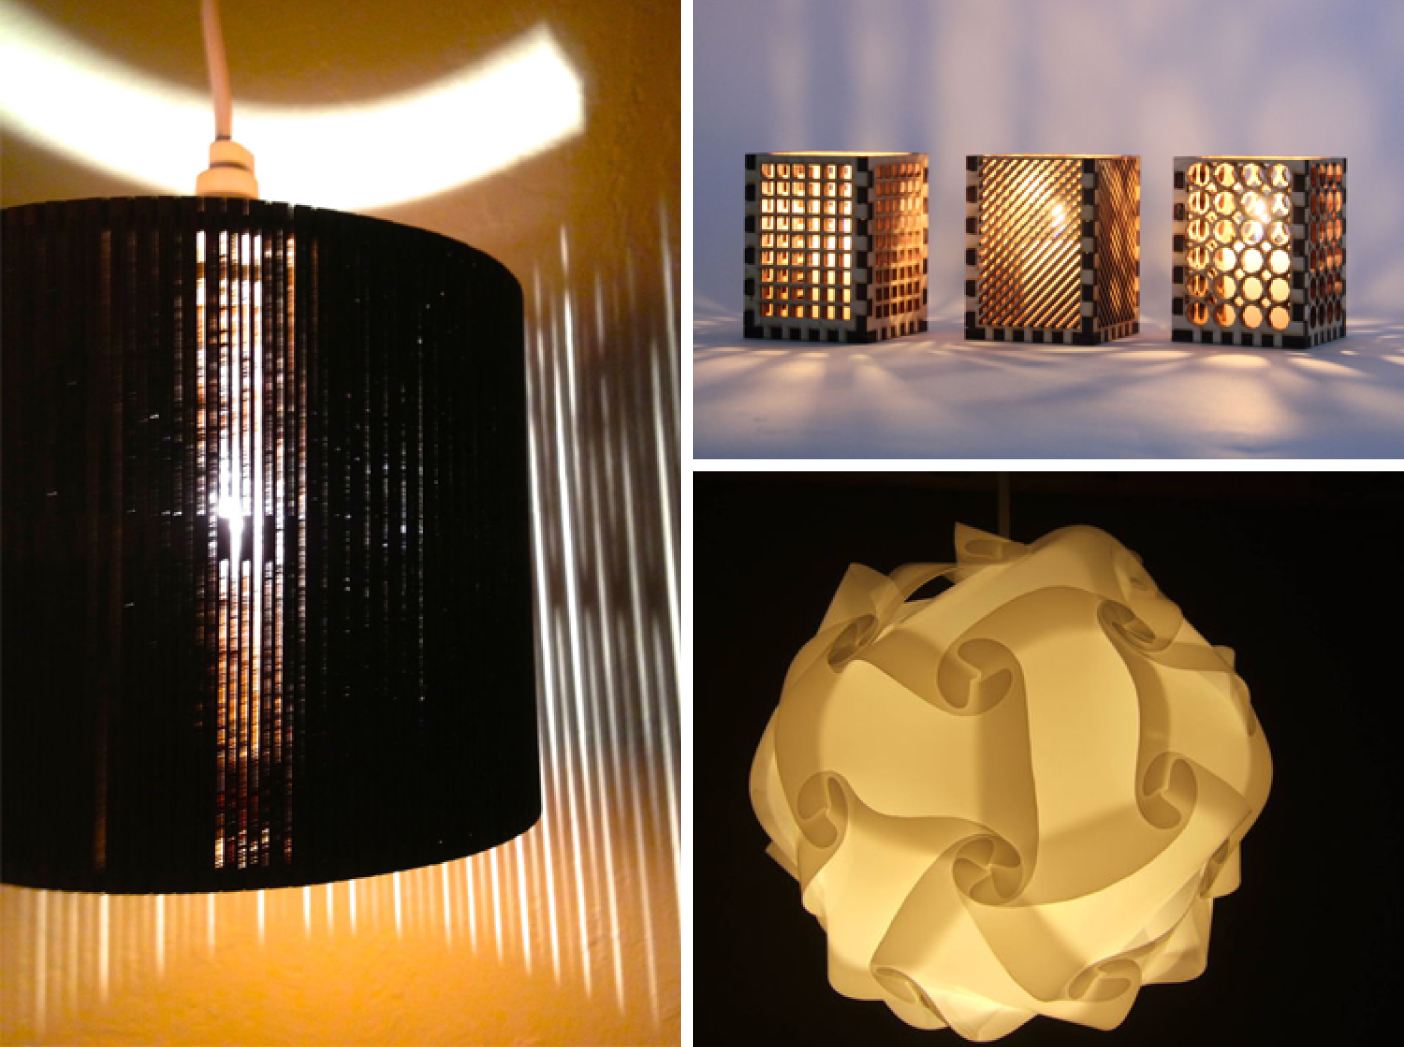
\includegraphics[width=6.5in]{images/instructables_lamps.png}
\caption{a selection of laser cut lamps from Instructables}
\end{figure}
\end{center}
\section{Motivation}
There is a precedent for creating DIY lamps through digital fabrication. The Instructables community tutorial website has an entire section devoted to DIY lamps, and many examples of patterns that use a laser cutter for fabrication. The majority of these examples do contain little creative flexibility by requiring the creator to emulate the design provided by the the tutorial. The tutorials that encourage deviation from the original design often require the person creating the lamp to use professional CAD tools. In one popular laser cut lamp instructable, the author recommends using Solidworks to design the form and Illustrator to create the pattern on the shade\cite{instructables_lamp}. SolidWorks is more difficult to use than illustrator, but has the benefit of being parametric. Conversely, Illustrator contains support generating aesthetic forms and patterns and is well suited to creating individual illustrations for laser cutting, but lacks the parametric functionality needed for the design of artifacts with multiple parts.
\begin{center}
\begin{figure}[h!]
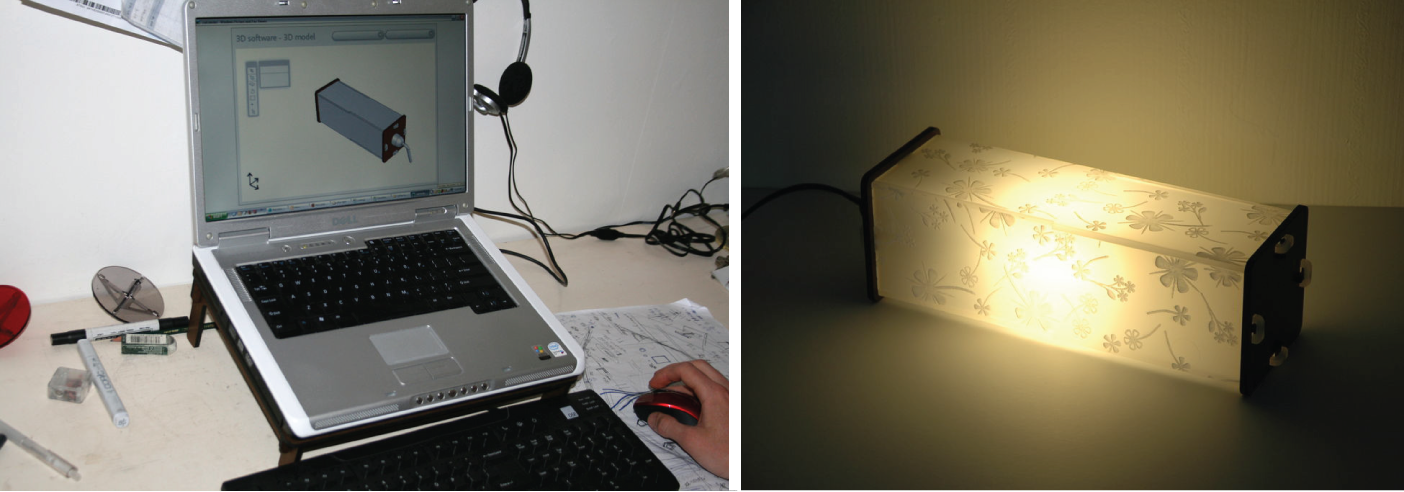
\includegraphics[width=6.5in]{images/solidworks_lamp.png}
\caption{Instructables lamp tutorial with SolidWorks design process}
\end{figure}
\end{center}
Using existing software tools for lamp design also presents other challenges. One common way to make laser-cut 3D forms is by assembling 2D press fit pieces. I found that when creating 3D forms that were curved, it was extremely challenging in 2D-CAD software to correctly size and design parts which would fit the faces of the lamp frame, creating the lamp shade. The shades themselves provided an excellent space for incorporating aesthetic illustrative elements into the lamp. Without parametric functionality however, simultaneous iteration on the aesthetics and form of the lamp is difficult. Computational design offered a solution to many of these problems, while simultaneously offering a form of constructive engagement in programing, fabrication and craft.

\section{Tool Description and workflow}
The first version of Codeable Objects attempted to combine parametric manipulation, aesthetic pattern generation and the conversion of a 3D form to 2D parts into a single computational design tool for lamp design. The lamp itself was comprised of 5 basic parts, a wooden press fit frame, a set of vellum pieces that fit over the frame to act as a shade,a set of cardstock pieces with a pattern that fit over the shades, and a pre-made standard light fixture that fit into the frame (see figure: \ref{fig:lamp_parts}.)
\begin{center}
\begin{figure}[h!]
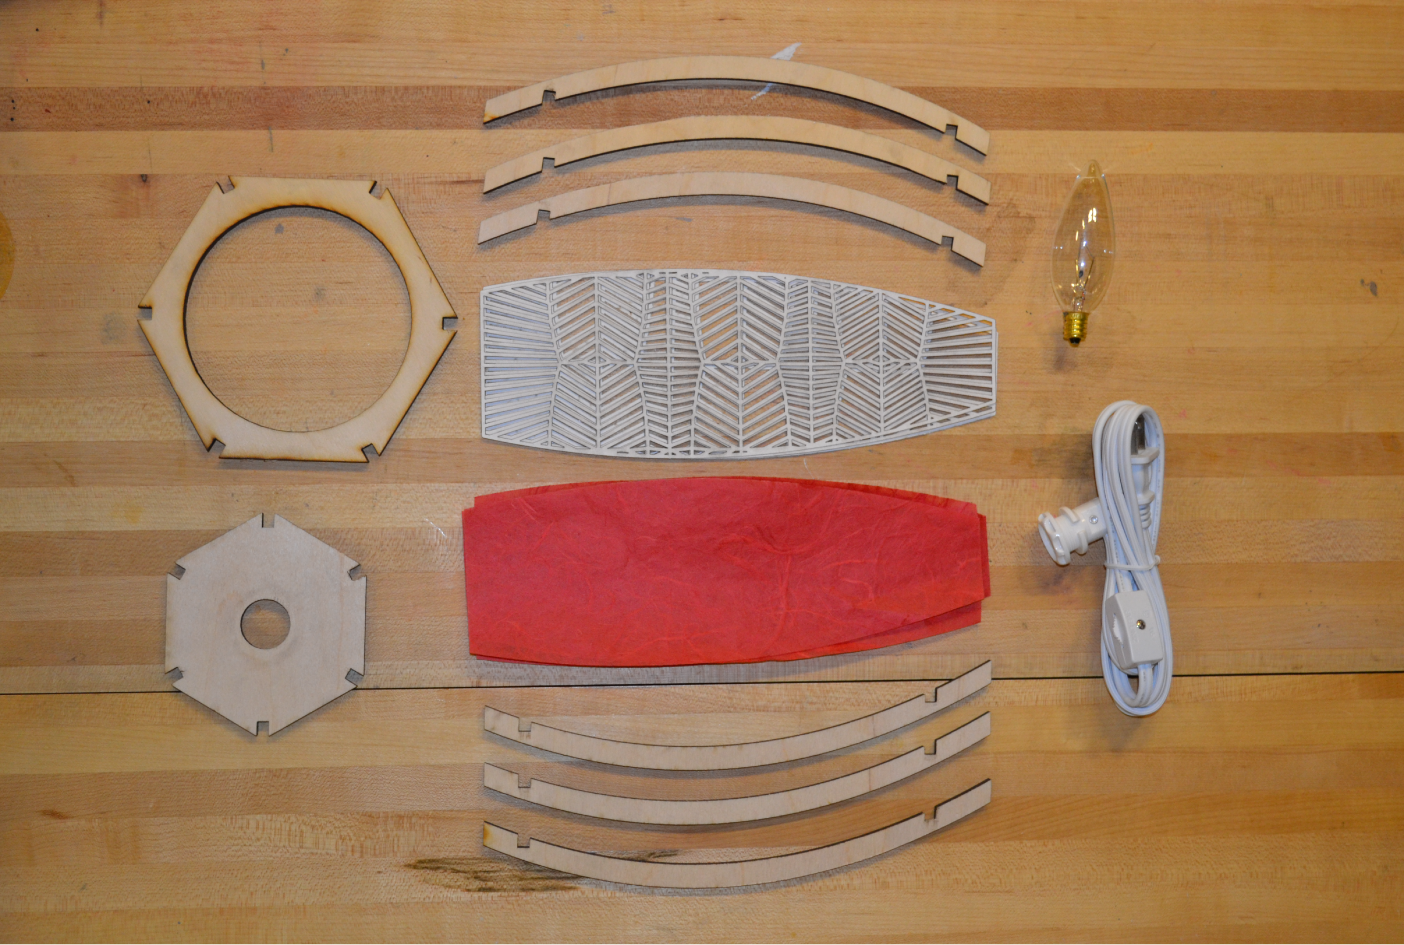
\includegraphics[width=6.5in]{images/parts.png}
\caption{the individual parts of a lamp}
\label{fig:lamp_parts}
\end{figure}
\end{center}
Codeable Objects was developed as a programing library for Processing and contained a set of programing methods that allow the user to describe the lamp, and define the tool paths for all three materials. In the first version of the library, all design took place via textual programing, and keyboard commands.  Within the Processing IDE one imports and initializes the controller class of of the Codeable Objects library, and uses it to call four main functions that determine the height, top width, middle width and bottom width of the lamp. These 4 parameters are used to calculate the equation for a parabola via 3 intersection points. Rotating this parabola around the y-axis generates a closed 3-dimensional form.  The library also provided access to an additional set of methods that control the number of sides, the resolution of the curve and the position of the internal structural supports. To facilitate the construction process, notches are automatically generated in all of the parts to allow the lamp to be press-fit together. The inclusion of this feature gives the user freedom to customize the shape of their lamp, without having to worry about the mechanics of construction. The library determines the correct position of the notches by calculating appropriate angle for each individual notch and determining the correct edge of intersection for each tool path based on this angle.  

 Codeable Objects also includes a second set of programing methods that allow users to describe the  decorative components of the lamp by specifying coordinates in polar or cartesian space. Upon compilation, the coordinates are used by the application to calculate a design using a Voronoi diagram. A Voronoi diagram is a geometric subdivision of space that generates a quadrants based on a given point set according to the equidistant boundaries between all the points \cite{deBerg}. When the diagram is calculated, each segment is checked for intersection or containment with the polygon. Segments with both endpoints within the polygon are preserved unchanged, while segments with only one endpoint inside the diagram are clipped at the appropriate edge of intersection, by checking their angle against the angle of the points of the edges of the boundary. Segments which have both points outside of the polygon are checked for intersection using the segment intersection algorithm and either clipped according to their intersection points or removed altogether if they lack an intersection (fig: \ref{fig:voronoi_clipped}).
 \begin{wrapfigure}{r}{0.5\textwidth}
  \vspace{-20pt}
 \begin{center}
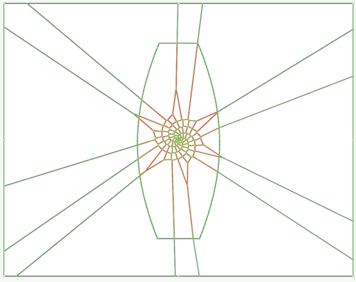
\includegraphics[scale=0.5]{images/voronoi_clipped.png}
\end{center}
\caption{Algorithim for constraining the voronoi diagram within the shade}
\label{fig:voronoi_clipped}
  \vspace{-10pt}
\end{wrapfigure}
  
Once the code is compiled, a graphic preview is displayed. For the pilot version, users could use key-commands to toggle between a view of the form of the 3D form of lamp, the voronoi-diagram pattern, and a 2D preview of the press fit parts (fig:\ref{fig:codeable_objects_v1}.) A final key-command allowed for the resultant design files to be exported as three separate pdfs, containing the paths for the press-fit frame, the shades, and the pattern files. 

\begin{center}
\begin{figure}[h!]
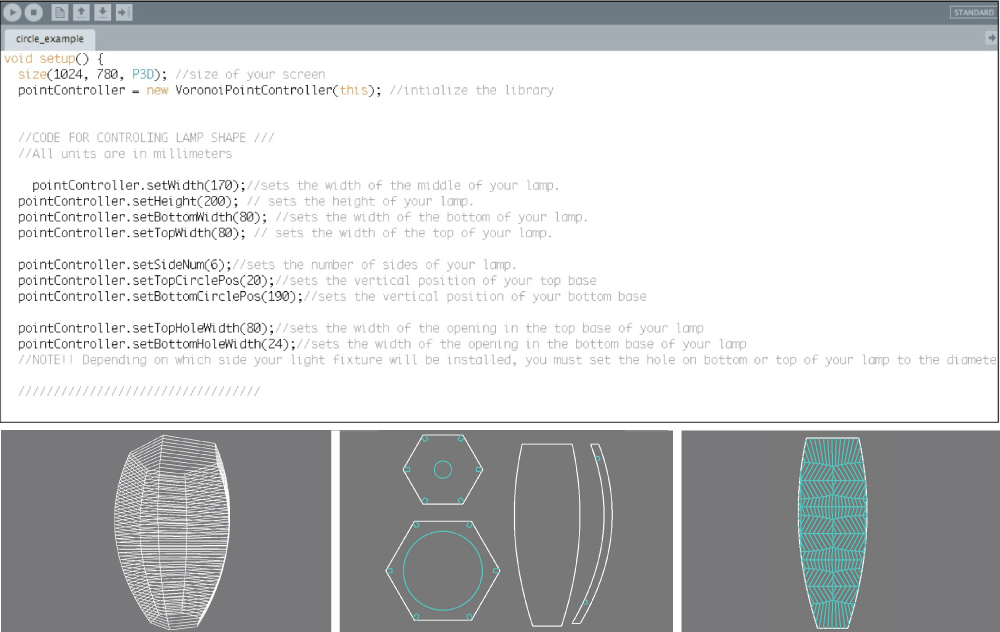
\includegraphics[width=6.5in]{images/codeable_objects_v1.jpg}
\caption{The first version of Codeable Objects, with only text-based interaction}
\label{fig:codeable_objects_v1}
\end{figure}
\end{center}
		
\section{Evaluation}
Using this basic pilot library, the first evaluation of Codeable Objects was conducted with a group of nine graduate students, ranging in age from 24-34, who engaged in a six-hour workshop. Five participants were women.  According to self-reported pre-survey data, all but one of the participants were intermediate to experienced programmers. Five of the nine had previous experience with Processing. In contrast, participants indicated they had little or no prior experience in design.  What experience they had was primarily gained in high school art classes and college elective courses. 

During the workshop, each participants engaged in the design and fabrication of their own lamp. Participants received programing instruction in the use of Codeable Objects and a basic explanation of the principles behind the geometry of the lamp. The pilot version of Codeable Objects was packaged with a set of example programs that contained the basic code for initializing the library and defining the parameters of the lamp, along with a variety of point generation methods. Examples included algorithms to generate spirals, circles and grids in points. Participants were also provided with access to materials, and received training in the use of the laser cutter. They given approximately four hours to design the structure and ornamentation of their lamp, followed by two hours for fabrication and assembly.

\begin{center}
\begin{figure}[h!]
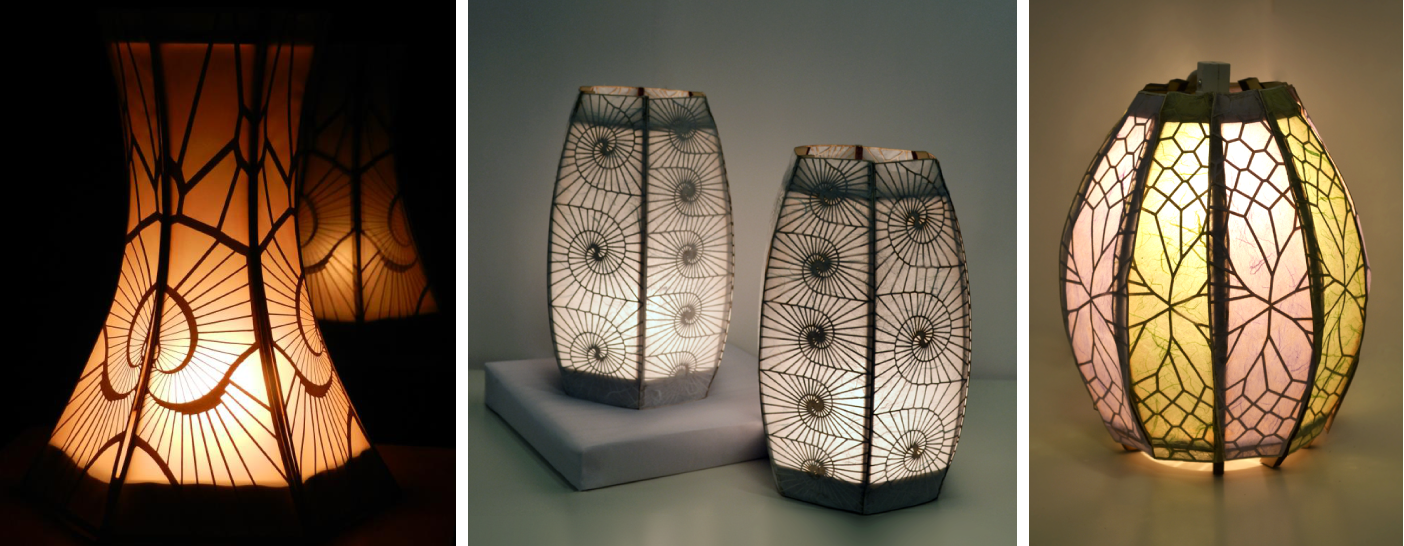
\includegraphics[width=6.5in]{images/finished_lamps2.png}
\caption{Several of the finished lamps from the first workshop}
\label{fig:finished_lamps}
\end{figure}
\end{center}

\section{ Results}
All but one of the participants in the lamp workshop successfully completed their lamp. The one exception was a user who wished to incorporate a specialized light fixture into their piece, but unfortunately damaged her parts while waiting for the fixture to arrive. Participants with little or no prior programing experience primarily relied upon tweaking or remixing the example programs to design the form and pattern of their lamp, whereas those more experienced in programing experimented extensively with the library to produce a wide range of forms and patterns. One participant wrote a program that decomposed a black and white image into a point cloud and used that as the basis for her pattern. Another participant wrote a program that used a Gaussian distribution of points to achieve the gradual variation he desired in his final pattern. 

 The physical assembly process required additional time beyond the duration of the workshop for most participants. This can partially be attributed to the bottleneck on the laser cutter, however the design and crafting components of the project took also longer than expected. Despite this, all the participants returned after the workshop to complete their projects, and each participants indicated on the survey that they were able to complete a finished product to their satisfaction. The physical objects produced were both attractive and functional; participants displayed their lamps in their offices and homes after completion. One participant returned several days later to build a second lamp so that he would have a matching set for his bedside tables (figure:\ref{fig:finished_lamps}.)		
		
		
\section{Discussion}

%The most evident success of the pilot version of Codeable objects was the high rate of project completion. This success rate was closely connected to the ability of the library to correctly constrain the design parameters of the lamp. Although participants at times had to re-fabricate parts due to incorrect settings on the laser cutter or variations in the physical materials, at no point did a participant have to re-fabricate their piece due to errors in the design itself. Once fabricated, all participants pieces fit together correctly. This success came at the cost however, of significant design limitations. Participants who wished to modify the form to have more than one curve, or create patterns that went beyond the restrictions of the Voronoi diagram had to resort to post-processing their design files with a different CAD tool. In general, the %

Because of their prior expertise, the experiences of the majority of the participants in the first study are not indicative of the feasibility of Codeable Objects for novice programmers. Their experiences instead stand in contrast to the experience of the novice coders in the successive workshops and provide important information about the usability and workflow of the software. Some of the experienced programmers provided immediate practical assistance by developing new example programs for Codeable Objects, including an extremely popular program for cosine and sine pattern creation. Because the library was open-source, they were also able to submit upgrades to the interface design and functionality, which were later incorporated into the core version.

The experienced programmers in the lamp workshop exhibited limited knowledge of computational design prior to the start of the workshop. When asked in the pre-workshop surveys how they thought programing, design and craft could be combined, the general response was either uncertain, or as method to create dynamic interactivity, rather than a tool for the design of form and pattern:
\begin{flushright}
\textit{``You can combine software and hardware and make craft more dynamic (e.g. sensors)."}
 \\Lamp Participant pre 1
\end{flushright}
\begin{flushright}
\textit{``[Programing] gives [you] the ability to make something dynamic."}
 \\Lamp Participant pre 3
\end{flushright}
Following the workshop, the participants were generally pleased with the creative affordances of the tool, and described how the software enabled them to expand their programing abilities to the realm of art and craft with greater success: 
\begin{flushright}
\textit{``I think programming makes designing more accessible because you don't have to be able to draw or paint."}
\\Lamp participant 4
\end{flushright}

\begin{flushright}
\textit{``I love the idea of being able to combine my interest in programming for creative expressions."}
\\Lamp participant 6
\end{flushright}

There was also an awareness among several participants about the practical benefits of combining computational design and digital fabrication:

\begin{flushright}
\textit{``I understand now how programming can be used for quick prototyping and mockups that can be used to inform final design decisions. This is easy [and] helpful when using physical materials where mistakes can be costly."}
\\Lamp participant 2
\end{flushright}

\begin{flushright}
\textit{``Using programming in the design process adds some exciting and unique capabilities over traditional design and crafting, including mixing in different algorithm and ideas from other existing software, and rapid prototyping of complex designs."}
\\Lamp participant 6
\end{flushright}

Following the workshop, one participant remarked that she had always believed that she was terrible at art, but that making the lamp had altered that perception. Although the primary objective behind Codeable Objects was to make computational design more accessible to non-programmers, in the first workshop, it provided a pathway for programmers to apply their skills to design and craft. From these responses, it is apparent that even among experienced programmers, algorithmic craft has the potential to expand people's understanding of the applications of programming and motivate them to apply computation to other forms of production and expression.

There were also elements of the process that were problematic for the participants. It became immediately clear during the workshop that textual programing was not the best method to design the form of the lamp. Many of the participants became frustrated about having to set the parameters and then wait for the compilation process to complete before they could view the resulting form. This issue was addressed partly in subsequent versions of the tool by replacing the textual parameters with a set of sliders in the compiled application, which would adjust the form in real time, across each of the views (figure: \ref{fig:slider_interface}.)
\begin{center}
\begin{figure}[h!]
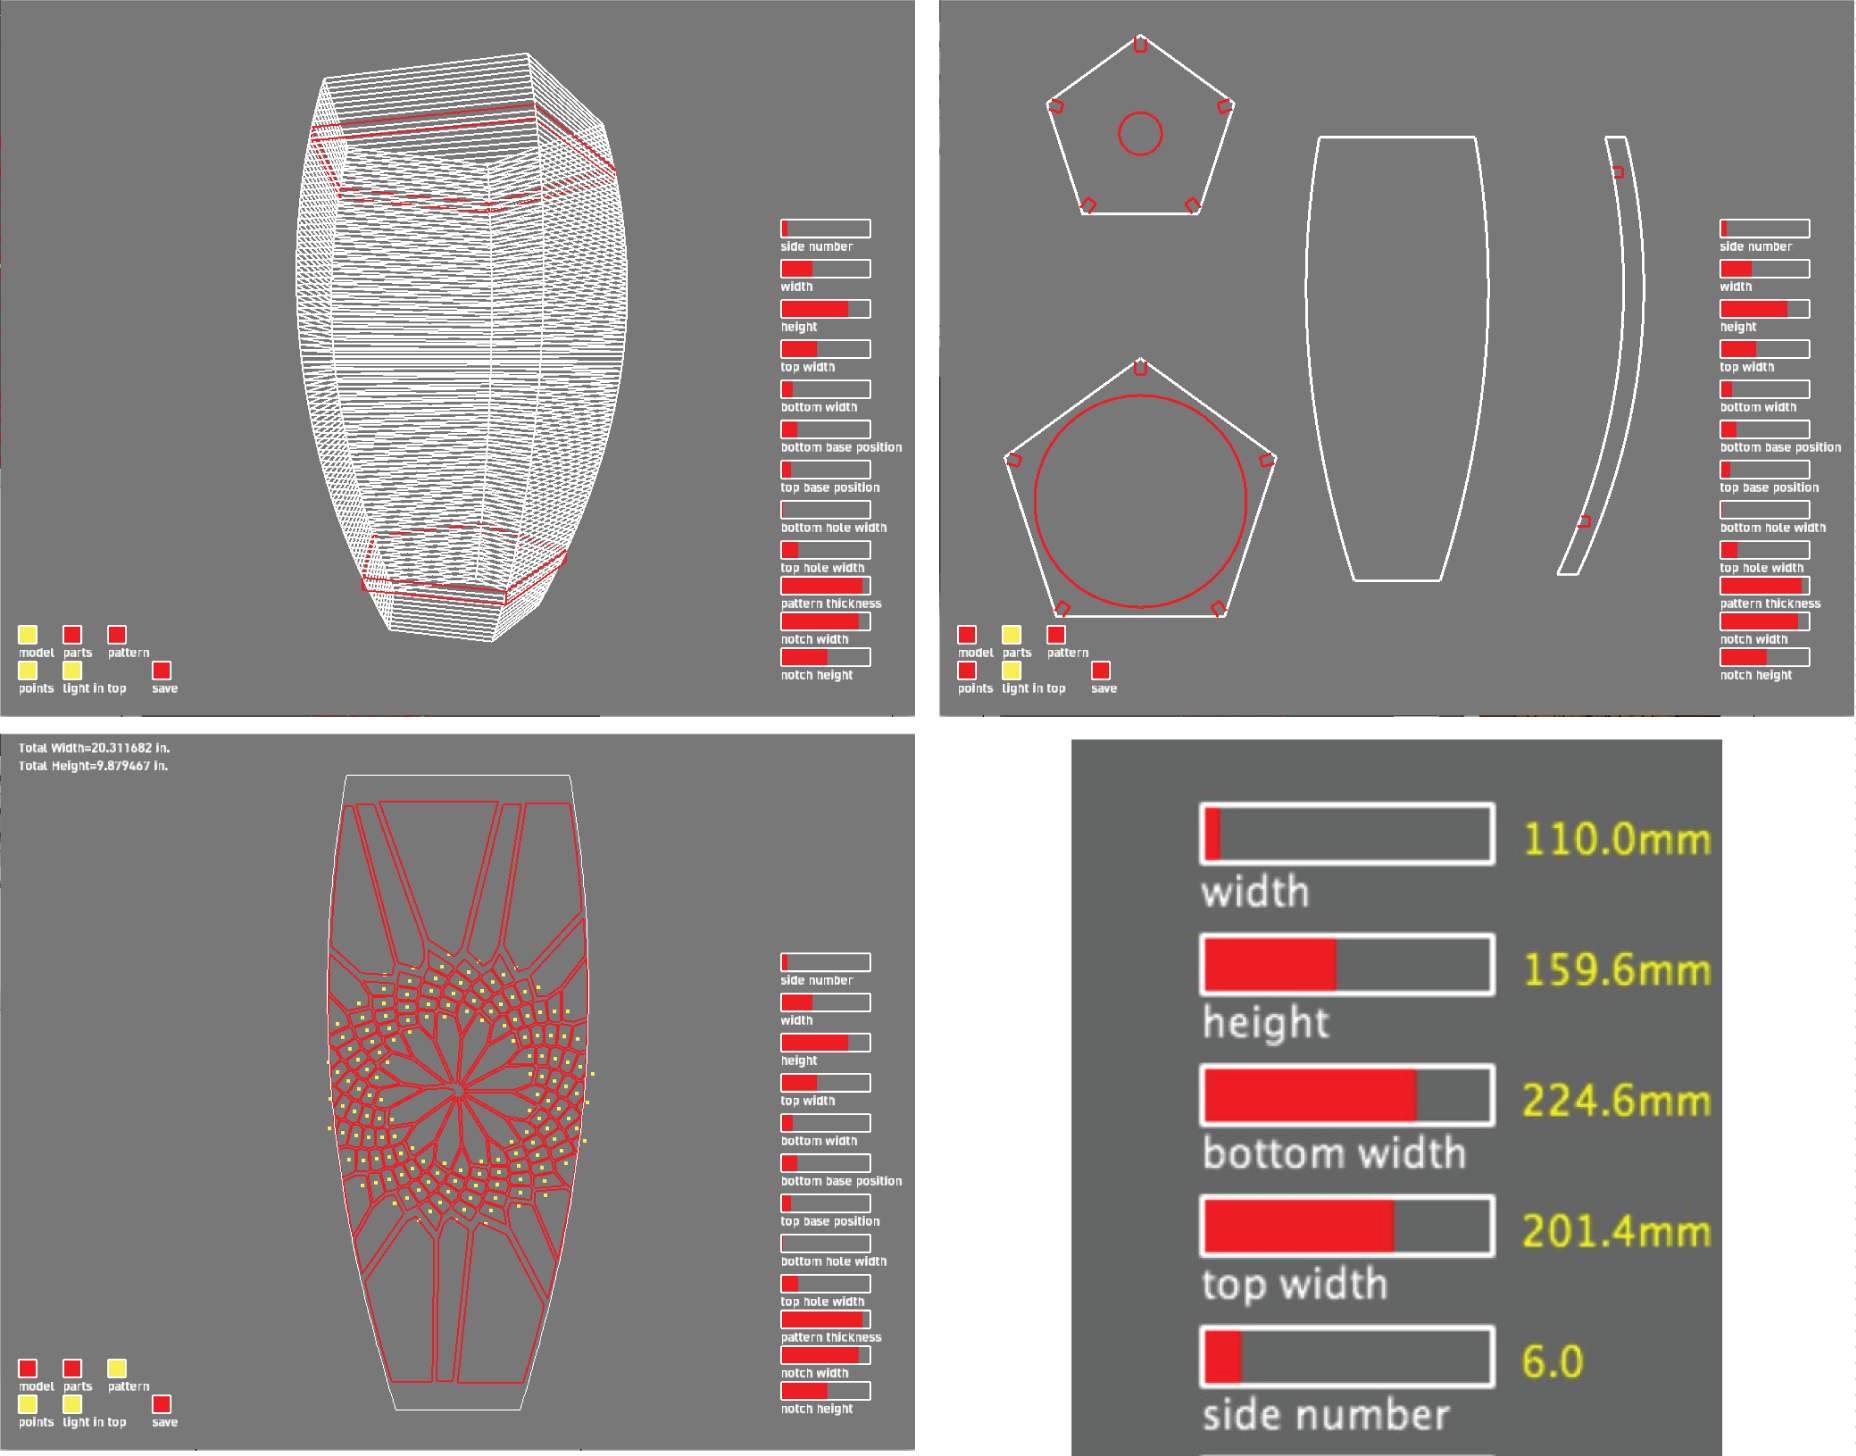
\includegraphics[width=6.5in]{images/slider_interface.png}
\caption{Revised graphic view with sliders}
\label{fig:slider_interface}
\end{figure}
\end{center}

The textual programing method was useful for creating pattern on the shades. The simple method of specifying points in a programing context provided a space for creativity and resulted in greater variation in the lamps. If the tool had relied on a more standard set of graphical user interface(UI) components, like sliders to control the point generation, it is doubtful that the same range could have been achieved. On the other hand, it was clear that the less experienced programmers had more difficulty deliberately designing the patterns of their lamps, and relied primarily on adjusting and remixing existing examples. 

Several participants also put forth detailed critiques of the programming process, which brought into focus concerns about the practice of computational design itself. One participant reacted against defining the generative qualities of the Voronoi diagram patterns as a design method:
\begin{flushright}
 \textit{``Changing the parameters didn't always generate the pattern you have in mind. It was more like generating a few semi-random patterns and you choose one that looks good. It is rather a trying-and-choosing rather than designing /making something you planned to have. I think "design" involves "intention" and "planning." Programming, crafting, and design should be combined in the way that entails prior planning and intentions as opposed to cutting together the semi-random choices, which could be good but I wouldn't call that design."}
 \\Lamp participant 6
 \end{flushright}
 
As this quote indicates, the attributes of randomness and generativity do not automatically lead to optimal or good design decisions. Some deciding factor has to play a role in the process, but the criteria for this decision are often ambiguous. This criticism touches on a core debate about the role of conscious design and the restriction of intuitive creativity in computational practices. The emergence of comments like this are encouraging, because they reflect the engagement of the participants, not just with the task at hand, but in a critical evaluation of the  creative implications of this form of creation. 

This comment also highlights a key restriction of Codeable Objects. It can be argued that adjusting the parameters and input values to a system constitutes a form of design. The task of defining the algorithms that determine the system itself however, constitute a more interesting form of computational design. With Codeable Objects, the user is unable to modify the program which defines the range of forms and patterns that are possible, unless they alter the source code of the library itself. When evaluated as a tool for algorithmic craft, Codeable Objects could have done a better job of supporting some of the deeper components of computational design. The stylistic limitations contained in the tool most likely contributed to the high success rate in project completion, and the general attractiveness of the resulting projects. For future tools however, I worked to create a better balance of stylistic and computational openness and accessibility for new programmers. 

One other defining component of the Codeable Objects pilot workshop was the contrast between the the challenges in the computational design and digital fabrication and the challenges in crafting. The difficulties people experienced while designing and fabricating their projects were often discrete;  such as correcting for mathematical error in coordinate placement, or having the incorrect setting on the laser cutter. More complex problems arose in these contexts as well, such as confusion around principles geometric point placement, however they were problems that could be addressed through verbal instruction and explanation. The challenges encountered in the crafting session were of a material or physical quality.  People struggled with finding the best techniques for assembling the parts and finishing individual pieces so that the resulting product maintained an attractive appearance. Most participants were surprised at the amount of time required to complete the physical assembly, and were often frustrated when variations in the crafting process violated the precision and perfection of the digital design, and laser cut parts. 

Some of the frustrations in the physical construction process were addressed in subsequent workshops by creating a paper variation of the lamp that was faster and easier to assemble and required no gluing (figure: \ref{fig:paper_lamp}.) In addition, a feature was added to the software which to report the approximate material size required for a design, so that users could ensure their would fit on the bed of the laser cutter. 
\begin{center}
\begin{figure}[h!]
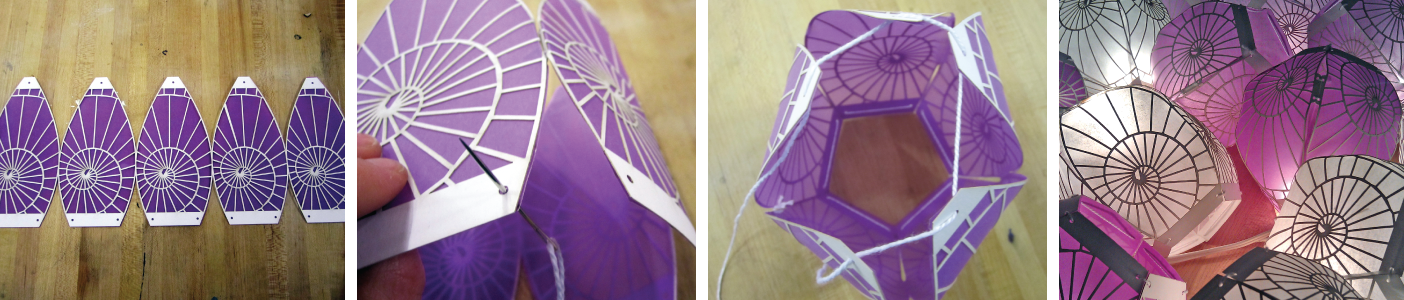
\includegraphics[width=6.5in]{images/paper_lamps.png}
\caption{The revised paper lamps}
\label{fig:paper_lamp}
\end{figure}
\end{center}
Although there is often an opportunity to improve a user's experience through changes in the interface and artifact design, some of the difficulties are embedded in the practice of hand-craft. In craft, it is both impossible and undesirable to eliminate the properties of material variation, and the benefits of practice and experience. Many of the difficulties workshop participants experienced in the crafting process do not reflect a failure in the tools, but rather challenges that are intrinsic to crafting, and best addressed through practice and familiarity with the materials. In this way, craft practice differs from computational practice. While programming benefits from experience and practice, the approaches for solving problems differ significantly. Programming often requires an analytical approach with an emphasis on consistency and regularity, whereas crafting requires a more intuitive process of responding and adjusting one's technique while in direct contact with the materials. Algorithmic tools should be presented in a manner that accustom users to operating in both discreet and intuitive modes of problem solving. Workshops that use these tools should attempt to merge craft and computational problem solving in a cohesive manner so that material experience informs computational approaches and vice-versa. 

\todo{this last section is unclear- re-write}
%% This is an example first chapter. You should put chapter/appendix that you
%% write into a separate file, and add a line \include{yourfilename} to
%% main.tex, where `yourfilename.tex' is the name of the chapter/appendix file.
%% You can process specific files by typing their names in at the 
%% \files=
%% prompt when you run the file main.tex through LaTeX.
\chapter{Soft Objects}
	
	\begin{center}
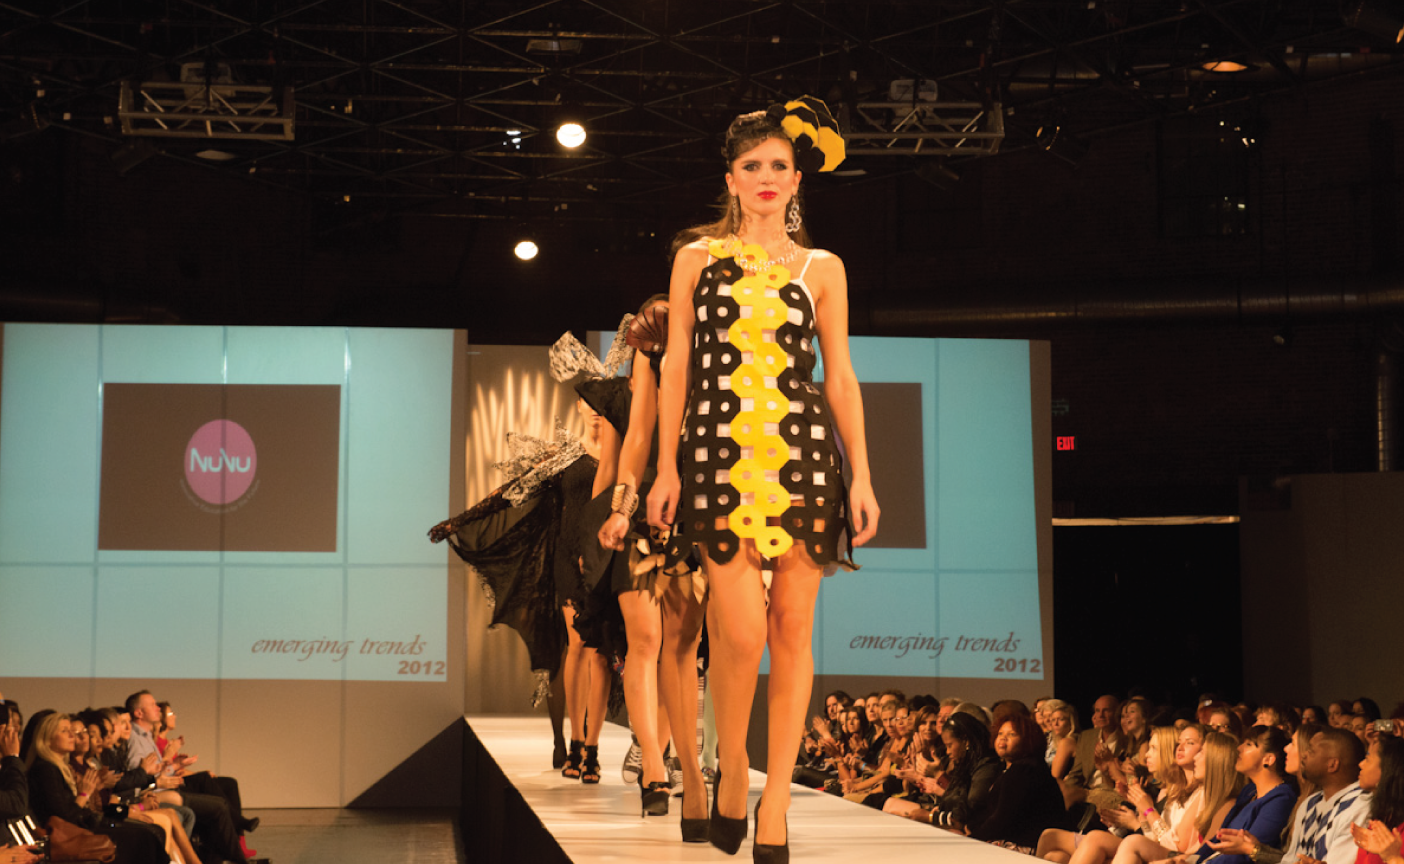
\includegraphics[width=6.5in]{images/fashion_show.png}
\end{center}
	
After an evaluation of the successes and limitations of the Codeable Objects library, I made an effort to modify the library in a way that would allow for a broader range of computational-design approaches and end products. In particular, I was interested in exploring the domain of algorithmically crafted garments and fashion accessories. Fashion is an exciting domain to connect to computation because it appeals to groups of people who are often under-represented in computer science, particularly females. Computational fashion design resonates well with algorithmic craft because it offers the opportunity to apply digital fabrication to textiles and fabrics, and because it introduces sewing and pattern-making as components in the construction process. Because garments and fashion accessories are created to be worn, computational fashion design requires the creator to consider questions of comfort, sizing and personal taste and and style when writing code.To support computational fashion design in the context of algorithm craft, I expanded Codeable Objects into a general programming library entitled Soft Objects and evaluated it over a 10-day workshop with young designers.


\section{Motivation}
With the growth in public awareness of digital fabrication, enthusiasm for fashion applications of digital fabrication technology is profuse. Much of this excitement is directed towards 3D-printed wearables and textiles. In July 2010, Iris Van Herpen released her Crystallization collection, which featured her first computationally designed, 3D-printed piece, marking the first time a 3D-printed garment had appeared on a fashion runway \cite{herpen}. Van Herpen and many other fashion designers continued using 3D printing as a medium for fashion. As a result, computationally designed, digitally fabricated fashion is often synonymous with 3D printing. The 3D-printed garments and accessories produced by professional designers like Van Herpen serve as inspiration for the future of digital fabrication and demonstrate wearable forms that would be impossible to create through any other means. For the average person, however, computationally designed and digitally fabricated garments of this nature present considerable limitations. Given current technology, cost and material, the majority of 3D-printed garments are impractical for every-day wear and require advanced fabrication techniques that are unavailable to many non-professional designers. Garments like the N.12 bikini designed by Continuum \cite{n12} are intended to be ready-to-wear, and available to consumers, but for the time being they are limited in scale, and still are costly. The construction of 3D-printed garments of this form appear to have little in common with existing methods of garment production, like sewing, knitting and embroidery. Admittedly, garments of this nature are inspirational and groundbreaking, yet individuals with sewing, knitting, weaving or others skills with textile manipulation may perceive their interests to be incompatible such forms of computational design and digital fabrication.

\begin{center}
\begin{figure}[h!]
\includegraphics[width=6.5in]{images/3D_prinited_high_fashion.png}
\caption{ 3D-printed fashion (from left to right: Crystallization 3D Top by Iris Van Herpen, Drape Dress by Janne Kyttanen, N12 Bikini by Continuum Fashion, Strvct shoe by Continuum Fashion}
\label{fig:high_fashion}
\end{figure}
\end{center}

Although perhaps less publicized than 3D-printed fashion, other  designers are merging fashion with computation and digital fabrication in a way that blends new technology with established approaches. Diana Eng's Laser Lace tee collection contains laser-cut machine-washable t-shirts with floral-inspired iconography. Further, her Fibonacci scarf is created through traditional knitting techniques, meshed with a Fibonacci knit pattern. Eunsuk Hur's modular fashion pieces are inspired by tessellations and fractal geometry. By creating garments through laser-cut interlocking pieces, Hur's stated aim is to produce items that are robust and durable, and also provide an opportunity for the user to engage in the creative process (figure:\ref{accessible_fashion}.)

These examples demonstrate a use of computational fashion design that is compatible with non-digital interests, and skill sets. Subtractive fabrication machines, like laser and vinyl cutters are dominant in this type of work because they work with traditional materials and can produce garments at  lower costs and larger scales than 3D printers. Variation in materials also can translate to a wide set of possibilities for hand crafting as well and different aesthetics and styles. It should be noted that accessible forms of 3D printing can produce compelling wearable objects; however the products produced are generally at the scale of jewelry and small accessories. Garments designed and produced as a blend of digital fabrication and textile materials and construction processes correspond well with the values and practices of algorithmic craft. The Soft Objects programming library was designed to allow new programmers to design the forms and aesthetic components of fashion accessories and garments through programming, followed by the physical construction of the garments using subtractive forms of digital fabrication and sewing. 

\begin{center}
\begin{figure}[h!]
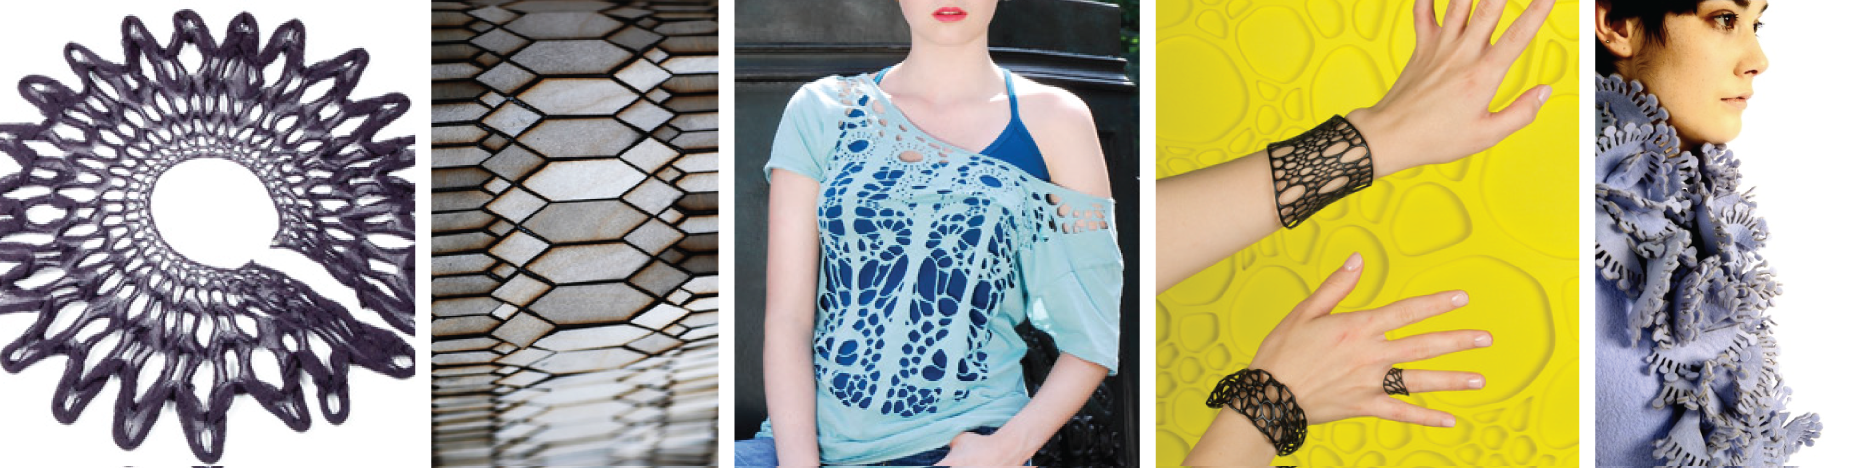
\includegraphics[width=6.5in]{images/accessible_fashion.png}
\caption{"Ready-to-wear" computational fashion (from left to right: Fibonacci Scarf by Diana Eng, Biomimicry laser-cut bracelet by Stefanie Nieuwenhuyse, Laser Lace All-Over Tee by Diana Eng, Interstice bracelet by Nervous Systems, Modular Fashion by Eunsuk Hur}
\label{fig:accessible_fashion}
\end{figure}
\end{center}
		

\section{Tool Description}
The Soft Objects library contains a set of methods that allows users to draw shapes and patterns and then export those shapes and patterns in a vector format that is compatible with x-y axis digital-fabrication machines. Similar to Codeable Objects, Soft Objects is used within the Processing programming environment and contains a set of programing methods that enable the design of visual forms and patterns. SoftObjects allows users to define and manipulate basic geometric primitives such as points, lines, curves, and polygons. These primitives can then be collected within Pattern and Shape objects---structures designed to capture surface decoration and 2D structure, respectively---to form increasingly complex designs. Soft Objects is formulated on an Object Oriented Programming (OOP) paradigm, which lets users create and manipulate collections of geometric primitives---Patterns and Shapes. This structure differs from Processing's drawing API, which uses a functional programming approach. Users are presented with a 2D preview of their designs when they compile their code. The structure of Soft Objects enables users to simultaneously apply transformations to all of the elements in a collection that make up a complex pattern or shape. The objective behind this structure is to open the design possibilities in a format that was suitable for creating complex 2D designs and aesthetic patterns for clothing and accessories, while ensuring that a user's designs would be compatible with subtractive fabrication. To simplify the process of garment creation, Soft Objects included functionality to import existing cut patterns as scalar vector graphics files (SVGs). This allows users to merge programmatically generated designs with patterns for pre-sized shirts, dresses and pants.

\begin{center}
\begin{figure}[h!]
\fbox{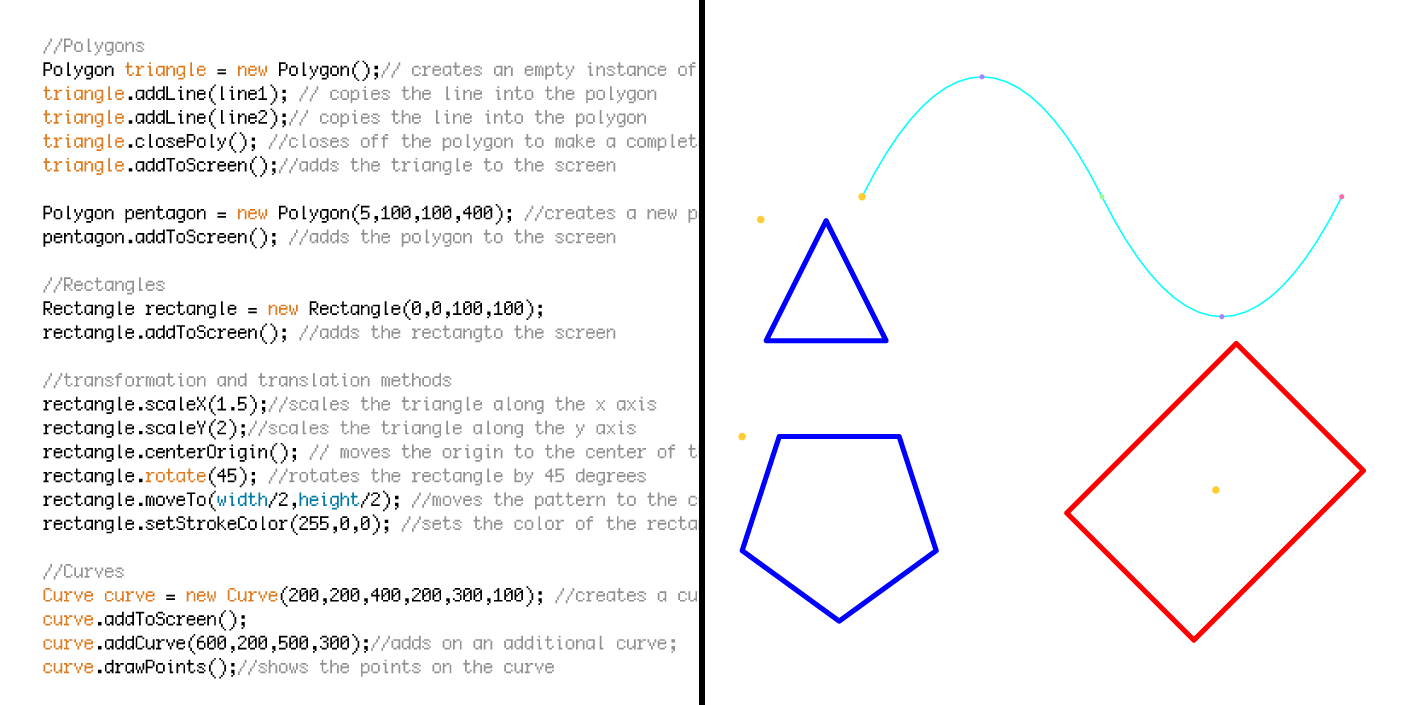
\includegraphics[width=6.5in]{images/primitive_syntax.png}}
\caption{Soft Objects primitives.}
\label{fig:softobjects_primitives}
\end{figure}
\end{center}
		
Soft Objects supports a variety of digital-fabrication machines by allowing users to save designs to PDF files. Output from Soft Objects can be fabricated on essentially any x-y axis tool. 3D structures can be created by assembling fabricated pieces. Figure \ref{fig:softobjects_workflow} demonstrates the workflow from code to a finished object. 
The Soft Objects library also contains a collection of pre-defined algorithmic patterns that can be initialized, including Voronoi diagrams, Koch curves, and L-Systems. It also includes an extensive set of example programs that users can modify and combine to produce individual results. These examples and pre-defined algorithms are useful to  expose new programmers to some of the complexity and variability that is possible through computational design. They also  demonstrate the abstract qualities of computation, without immediately requiring people to learn substantial amounts of programing structure and syntax. 		

\begin{center}
\begin{figure}[h!]
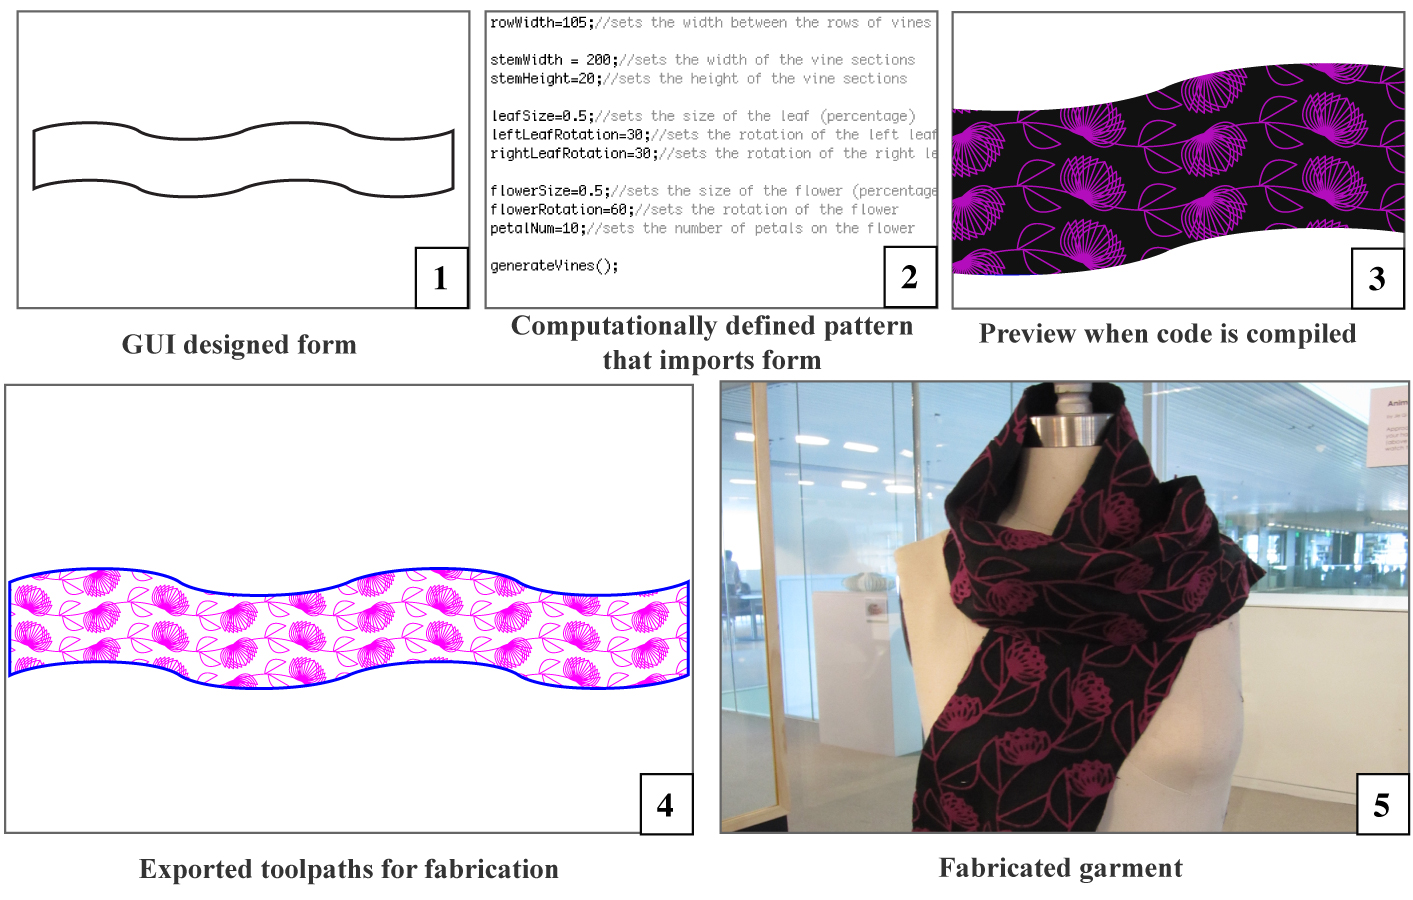
\includegraphics[width=6.5in]{images/softobjects_workflow.jpg}
\caption{Soft Objects workflow.}
\label{fig:softobjects_workflow}
\end{figure}
\end{center}
		
\section{Workshop}
The evaluation of Soft Objects was conducted during a 10-day workshop with a representative group of participants---eight young adults, ranging in age from 11 to 17 and composed of 75\% male and 25\% female. A significant majority (88\%) stated in pre-surveys that they had little or no prior experience in programming, and only one participant had prior experience in Processing. All of the participants indicated some level of prior experience in art, design, or craft. Most attributed their design or craft experience to art or drawing classes. The workshop was conducted at the Nuvu Magnet Innovation Center for Young Minds. Participants were given 10 days to conceptualize and construct a garment using a combination of computational design, digital fabrication, sewing and crafting. The workshop was more open-ended than the Codeable Objects workshop because participants could produce any type of garment they wished as long as components were computationally designed and digitally fabricated. During the workshop, participants were introduced to Soft Objects and the concept of computational fashion in a multi-step process that engaged participants in different levels of programming through the construction of different garments and accessories. First, participants were provided with a small set of example programs similar to the lamp workshop. This step allowed them to manipulate a core set of parameters to generate the pattern and form of a scarf, which they then cut on a laser cutter (figure: \ref{fig:scarves_bracelets}.) 

\begin{center}
\begin{figure}[h!]
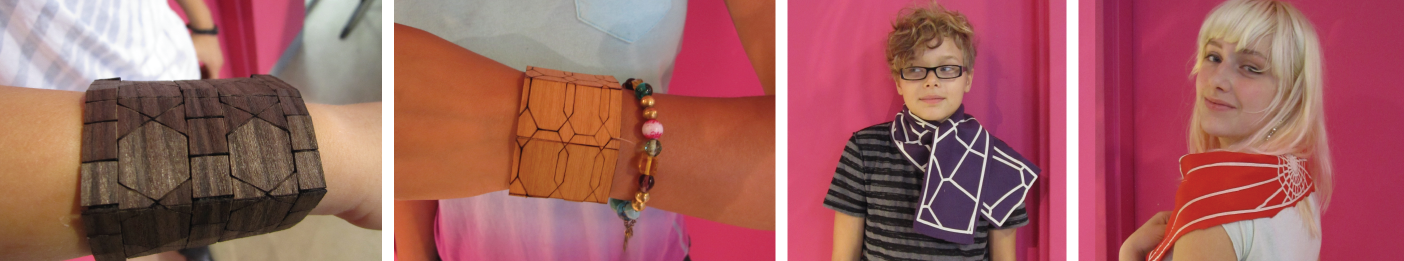
\includegraphics[width=6.5in]{images/scarves_bracelets.png}
\caption{Bracelets and scarves from preliminary activities.}
\label{fig:scarves_bracelets}
\end{figure}
\end{center}


Second, participants were instructed in a number of primary programming concepts, including iteration, function definition, and the use of variables and primitive data-types. During this instruction, participants were guided through the process of independently using Soft Objects and generating their own programs from scratch. They used these programs to create a design for a wooden bracelet (figure: \ref{fig:scarves_bracelets}), which was then laser cut and assembled. These initiation activities demonstrated the stylistic affordances and design properties of computational design and digital fabrication and  providing participants with the practical foundation to begin conceiving of and executing their own ideas. During the remainder of the workshop, the participants were asked to conceive of concepts and designs for their own garments. They were provided with the resources to design, prototype, and craft finished artifacts.

\section{Results}
Participants in the fashion workshop were successful in using programming and digital fabrication to design and produce finished garments. During initiation activities, participants independently wrote and compiled programs of  and produced physical products based on the design generated from their programs. With assistance the participants applied sophisticated programming methods to produce a diverse set of final products (figure: \ref{fig:fashion_results}). One pair of students developed an ``armor dress" by writing a program that geometrically described a single ``scale" shape, imported a dress pattern from Illustrator and filled it with rows of scales that corresponded with the dimensions of the dress. Another pair created a geometrically inspired dress with octagons and squares of different sizes that were laser cut from starched fabric. Another student created American-flag-inspired pants using a program that generated random orderings of red and blue stripes on a white background. One group that was less interested in the process of sewing clothing than other students created a program that generated a recursive virus-like pattern. Then they used screen printing to reproduce the pattern on pre-made  sweatshirts and t-shirts.

\begin{center}
\begin{figure}[h!]
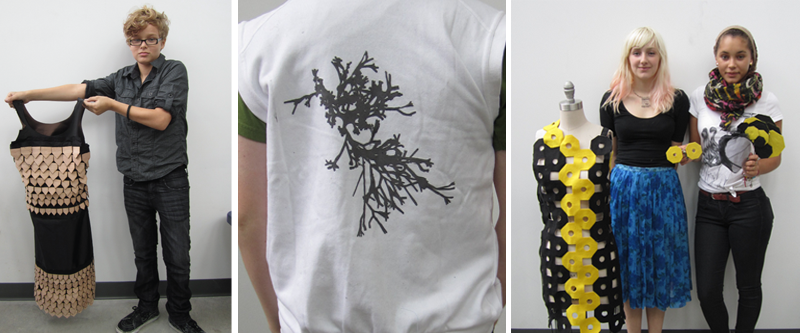
\includegraphics[width=6.5in]{images/fashion_results.png}
\caption{Completed garments (from left to right: octagon dress, flag pants, samurai dress, viral sweatshirt)}
\label{fig:fashion_results}
\end{figure}
\end{center}


On the post survey, when asked if they ``were able to complete a finished project to their satisfaction," 100\% of the participants responded in the affirmative. Their garments were attractive and functional, indicated by the fact that participants from the fashion workshop kept and wore their creations. Direct comparison of the pre-and post-workshop surveys also demonstrated that on average participants interest in crafting increased as a result of the workshop, as did their enjoyment of the design process. Eighty-eight\% of the participants in the workshop indicated that they felt more comfortable programming after the workshop than before.

\section{Discussion}
The Soft Objects workshop occurred over a longer time period than the Codeable Objects workshop, and explored a wide range of crafting and computational techniques. As a result, I had an opportunity to spend considerable amounts of time observing and talking with the participants. Because the participants were novice programers, their experiences better reflect the target demographic of this research than in the Codeable Objects study. Through this workshop I confirmed that algorithmic craft activities can actively support the expression of personal identity among young designers. The workshop activities fostered feelings of confidence in programming and supported aesthetic and technological literacy. They also promoted a deep understanding of computation as evidenced by critiques of the participants and demonstrated the importance of physical prototypes in the design process. Finally, the workshop promoted a sustained engagement in programming.

 
\subsection{Identification as a Programmer}
Similar to the participants in the Codeable Objects workshop, the fashion participants began with vague ideas about the applications of computation. When asked in the pre-workshop surveys how they thought programming, art and craft could be combined, participants responded in writing in the following ways:
\begin{quotation}
\textit{``To be honest, I am not too sure how it would all be combined because I don't know much about programming."} 
\\Fashion Participant Y

\textit{``With programming, we can make programs do things for us."}
\\Fashion Participant J
\end{quotation}

In addition, the participants had almost no prior knowledge of computational design. Those participants who had some with prior programming experience associated it largely with interactivity and actuation:
\begin{quotation}
\textit{``I would love to combine things like T-shirts and speakers or other different types of technologies."}
\\Fashion Participant J
\end{quotation}

Following the completion of their final projects participants were much more descriptive about the applications of programming:

\begin{quotation}
\textit{``I think [programming and fashion] are really interesting but I never thought they could ever be together in one concept, and it's awesome that I know that now- that you can design aesthetically pleasing things from coding."}
\\Fashion participant K


\textit{``I've never thought of programming as physical; I thought it was only in computers. But then when we made the scarves and stuff, I thought that was really fun."}
\\Fashion participant M
\end{quotation}

Many people also expressed a growing confidence in their ability as programmers. During the interviews, several separately stated that that while they did not feel completely comfortable programming independently, the experience made programming feel significantly more accessible:
\begin{quotation}
\textit{``For someone who never had any programming explained to them before, when you look at [computational drawing examples] it feels really inaccessible, but now that I've been taught a little bit of [programming], I can kind of crack at the walls a little bit and understand how it works, and that makes it more accessible to me."}
\\Fashion participant S

\textit{``Even though now I'm not really a Processing expert now, I've just experienced it and it's not as scary to me, like the idea of coding, you just kind of have to learn some stuff and practice it more, but I think I definitely understand the concept of it."}
\\Fashion participant K
\end{quotation}
Finally, the programmers in the fashion workshop expressed feelings of pride and a sense of accomplishment in their new-found programming skills:
\begin{quotation}
\textit{``I'm actually kind of proud. I know what's going on. It feels different... I just thought [programming] was just about these huge programs that you have to piece together, and that you have to be really, really smart to do it, but I can do it."}
\\Fashion participant P

\textit{``I think it was really cool that we used [programming] for fashion, cause I think a lot of people might think people who do fashion aren't really smart or something, and then they think that people who design code are like brilliant coders and can do really awesome stuff with it."}
\\Fashion participant K
\end{quotation}

 The confidence, sense of belonging, and personal agency demonstrated in these comments stand in contrast to popular views of programming as specialized and inaccessible. These sentiments indicate that introducing programming in the context of algorithmic crafting not only has the potential to change people's understanding of the relevance and applications of computation, but also promote a personal awareness of technological literacy and competence. 
 
\subsection{Application of Computational Affordances}
Aside from a general understanding of the potential applications of computation, participants were able to leverage the advantages of computational design in their final projects. For example, the octagon dress used parametric design principles, which was evident because participants were able to change the size and orientation of the octagons in the dress by modifying several parameters at the start of their program to affect the entire pattern, rather than rotating and adjusting each shape independently. The samurai dress took advantage of the computational properties of precision and automation. With help from an instructor, the creators programmatically generated an individual vector file for each row of scales of the dress, expediting the production process (figure:\ref{fig:samurai_dress_progression}.) The samurai dress is particularly interesting because it shows a remarkable  transition from the design expressed in original concept art by the participant and the final garment, demonstrating  adherence to the person's creative vision through computation. Lastly, the viral shirt, demonstrated an application of generativity. The aesthetic of the viral pattern was produced using a weighted random-number generator to determine the number and length of the branches in each recursion of the pattern. Although the implementation of the weighted number generator was facilitated with help from the instructor, the participants came up with the idea of using it on their own.
\begin{center}
\begin{figure}[h!]
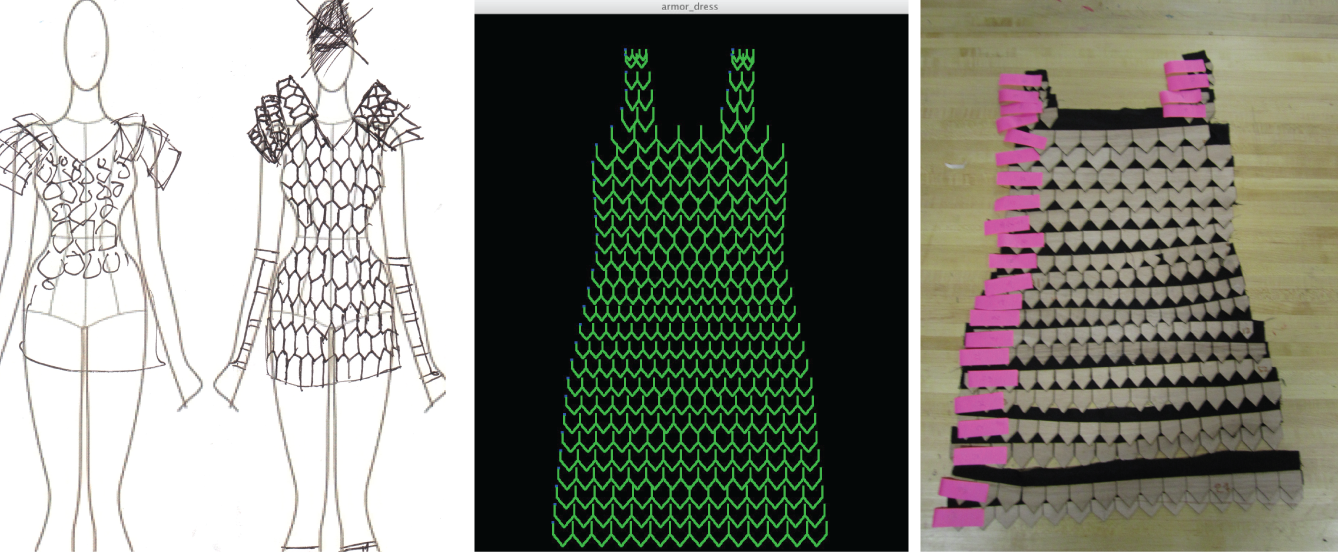
\includegraphics[width=6.5in]{images/samurai_dress_progression.png}
\caption{Progression of samurai dress (from left to right: concept sketch, computationally generated pattern,laser-cut components of final garment)}
\label{fig:samurai_dress_progression}
\end{figure}
\end{center}

Many of the participants demonstrated an understanding of the rationale behind the methods they were using. One of the creators of the armor dress compared the process of programming the design of the dress to that of manually drawing it: 

\textit{``With drawing you can achieve everything programming can, but I would prefer to program it. [programming] can be pretty convenient...the computer is helping me. Like if you want to make pizza, the computer is like a pre-made crust."}[Fashion participant E]

Participants also articulated an understanding of specific programming functionality. One participant described the point at which she understood the application 
of parameterization:

\textit{``One moment that stuck out was when you helped me make a code with original geometry that could be changed so that when you changed one thing it changed everything and that was cool because I felt like I actually made something that could be changed and then applied."}
[Fashion participant K]

The ability to understand and describe how computation supports creative objectives is essential in motivating an individual to spend time learning and implementing these methods. Once the aesthetic possibilities of the recursive viral pattern were apparent to the designers, they became engaged in understanding the underlying algorithm so that they could produce a pattern to their exact specifications. Algorithmic craft can provide the motivation for participants to tackle complex computational problems with sophisticated approaches when problems are clearly grounded within the design objectives of the individual. A continual challenge in engaging new programmers in algorithmic craft is  selecting programming approaches that allow for compelling aesthetic and design possibilities but remain approachable for first-time coders. 

\subsection{Aesthetics and Identity Expressed Through Code}
The fashion workshop provided the opportunity for participants to use computational aesthetics as a way to express their personal style. Fashion can serve as a means of self-expression and for conveying one's identity. Discussions about fashion conducted at the start of the workshop indicated that participants were aware of the connection between fashion and identity and were eager for opportunities to create clothes that expressed their style. As a result, the majority of the garments created in the workshop contained an expression of the fashion sense of the participants who created them. For example, the participant who created the flag pants was very explicit that the pants have some form of an American flag motif, but not resemble the traditional, and as he put it ``tacky" flag pants that he commonly saw. He wanted his flag pants to be ``something that he would actually want to wear." His programming choices were made in direct consideration of his desire to create a pair of pants that he felt were fashionable.

When asked about the experience of making and designing his pants he said:

\textit{``[The workshop] definitely changed my impression of making clothes, I thought it was pretty quick to make clothes, but it actually takes a long time, and it's also really fun. I love the fabric I made."} [Fashion participant M]

His enthusiasm also was evident in the fact that after the pants were complete, he tried them on and wore them for the remainder of the workshop. This level of enthusiasm was common among participants; they all proudly modeled their creations, and many of them wore them home. This behavior suggests a relationship between the decisions made in a programming context and the participant's desires to express their visual identity. The participants were selective in the code they wrote to design their garments because they intended to wear the garments, and as a result, be represented by them. This powerful affective relationship between computation, design, and self-expression provides a natural way to engage people in programming and design by supporting their personal interests. 

\subsection{Physical and Digital Connections}

One of the challenges of algorithmic craft, alluded to in the Codeable Objects discussion, is that the practitioner must work between digital designs with physical materials and processes. Physical prototypes often serve as a key point of transition between these spaces. In the fashion workshop, prototyping played an important role, and demonstrated how computational tools can support and sometimes hinder the prototyping process. The focus on fashion made it possible to supply the participants with large amounts of inexpensive test fabric. The laser cutter could cut fabric much more quickly than thick materials, which allowed participants to produce numerous prototypes of their projects before creating a final piece. Most groups produced two or three prototypes, with one participant creating six iterations of a single jacket. This rapid production process formed a direct connection between discoveries made in the physical prototyping space and decisions in the programming realm. 
In the case of the octagon dress, (figure:\ref{fig:fashion_results}), the participants first cut test rows of octagons to determine the appropriate scale, then adjusted their design by modifying their program.Once they cut out a second more -omplete version of the dress, they rotated one of the shoulder straps on the physical prototype and formed an idea for a one-sided shoulder strap. They implemented this design change in the digital version of the dress by making additional changes to the size and rotation of the shapes defined in the code. When asked about this process in the interview one of the participants said:

\textit{``I think it was really fun that we got to do a prototype first because then if you don't like it, you don't feel a lot of pressure because you can make it again really fast, and there's no stress because if it doesn't turn out well, then it's not your final project.} [Fashion Participant K]

The combination of programming, rapid fabrication, and physical construction allowed for a design approach that transitioned from programming to fabrication to programming adjustments based on the fabricated elements, and then back to fabrication. This iterative approach resulted in a closely linked cycle of physical and digital engagement. 

 \subsection{Enthusiasm in Crafting and Coding}
One of the most encouraging aspects of following the fashion workshop, was the participant's enthusiasm and desire to continue making. Participants talked extensively about what they would like to make in future with programming, stating that they would like to continue making clothing, or other personal functional items like furniture and ``things they could use around the house." The experience of both sets of workshop participants also demonstrated the ability of these techniques to produce objects that were designed to complement personal items and living spaces. When asked what she would like to make if she continued to program, one participant responded: 

\textit{``Things like we're making now, things that you would want to keep or use, things that look nice as opposed to like computer games, or ``input-output" devices. I think those are fun, but it's not as cool as things that you can hold in your hand. I actually hung up the scarf I made in my room, and now I can be like ``I made this on Processing" and people will be like what? It's cool! "}[Fashion participant K]

This enthusiasm, combined with the high potential for individual expression and sense of accomplishment encouraged meto continue exploring fashion and garment production as topic space for algorithmic craft. While the fashion workshop highlighted many positives in this sense, I also encountered several areas for improvement. 

\section{Limitations}
The most evident barriers in the Fashion workshop involved the syntactic challenges of programming. Many participants expressed a frustration with the syntax in both surveys and in-person interviews. Although the workshop participants were able to generate their own programs, they required more assistance from an instructor to write some of the commands. In addition, a feeling of needing to memorize programming syntax frequently translated to a sense of frustration. One participant stated in an interview:

\textit{``I couldn't memorize things, so it also was frustrating for me to always have to get you to help me write the code."} [Fashion participant K]

Many people requested some form of written "cheat sheet" that listed the key methods and how to use them. They also pointed out that they often had to write a lot of code (including import commands as well as setup and draw functions), even for simple tasks. Writing code for the first time is always challenging; however the high levels of frustration registered by the participants often focused on aspects of programming that were extraneous to the design itself. Because I wrote Soft Objects as a Processing library, it required that the syntax correspond to Java, a difficult language for beginners. Java is a general application language and has many syntactic requirements that are unnecessary for computational design applications. Based on this difficulty I concluded that future algorithmic crafting tools should explore domain-specific languages that directly applied to design and fabrication.
 
Along with difficulties with the programming syntax, participants struggled with some of the post-processing techniques. In order to be suitable for digital fabrication, many of the participant's computationally generated designs required some post processing in Illustrator. Usually this required using Illustrator's shape boolean functionality to merge shapes or expand outlines so that the vector paths would correspond to the desired cut pattern on the laser cutter (figure:\ref{fig:illustrator_example}.) Although the methods to perform these operations were simple, they needed to be repeated every time the design was modified programmatically. This was not only inefficient but sometimes prevented people from determining if their designs were feasible for fabrication when they were in the programming environment. This difficulty encouraged me to focus on ways of removing the need for Illustrator from the process altogether so that all design modifications could be initialized and updated programmatically.

Many participants  also struggled with the concept of prototyping. These struggles were evident in practical aspects, such as participants not saving their programs and digital design files (despite repeated reminders from the instructors to do so). Participants also frequently spent too much time on assembling their early prototypes, and were they frustrated when they realized they would have to make design changes and repeat some of the manual labor. Although I took pains in the workshop to introduce participants to the concept of prototyping, these instructions were not always absorbed. This may present an opportunity for future algorithmic crafting tools to contain specific features to encourage and support the physical prototyping process. One possibility is to include simulation tools that preview the constraints and behaviors of physical materials. The value of working with physical prototypes should also be supported, however, by features that allow designers to scale their files and fabricate first in miniature, and by software that allows easy access and management of multiple versions of a design throughout the design process.
	
Finally, as in the Codeable Objects workshop, participants were frustrated by the delay between adjusting their code and seeing the results. Although, not an absolute solution to the challenges in learning programming syntax, a programming environment with quick feedback could assist with the issue of syntactic challenges by providing novice users with improved ways to visualize the effect their syntactic changes have on their design. The implementation of background compiling, the process by which code is automatically compiled and executed as changes are made, has been applied successfully in several tools for novice programmers, including Scratch and Alice \cite{alice}, and more recently with Khan Academy \cite{khan}. My reliance on the Processing for Soft Objects made the incorporation of real-time compilation infeasible, however that change quickly became a goal for future tools.

\section{Summary}
Participants in the Soft Objects workshop were able to create personal wearable items that were beautiful, functional, and personally meaningful through computational design, digital fabrication and craft. During the workshop, the participants learned new skills in programing and digital fabrication, as well as techniques for pattern-making and sewing. The participants emerged with an awareness of the applications of computational design for digital fabrication, specific understanding of some of the primary elements of programming, and a desire to continue using computation to build their own objects. Although there are many areas for improvement in future tools, the Soft Object workshop primarily demonstrated the importance of incorporating approaches that further reduce the practical challenges of programming. Possible approaches include removing extraneous syntax, reducing the number of programing methods, providing rapid and informative visual feedback, and adding features that help users make their designs feasible for fabrication. The objective of these features is not to trivialize the process of algorithmic craft, but to remove barriers to independent and deliberate creation through computational design, and to ensure the successful translation of digital designs to physical forms that are compatible with craft practices. 
%% This is an example first chapter.  You should put chapter/appendix that you
%% write into a separate file, and add a line \include{yourfilename} to
%% main.tex, where `yourfilename.tex' is the name of the chapter/appendix file.
%% You can process specific files by typing their names in at the 
%% \files=
%% prompt when you run the file main.tex through LaTeX.
\chapter{DressCode}\label{sec:DressCode}

\begin{center}
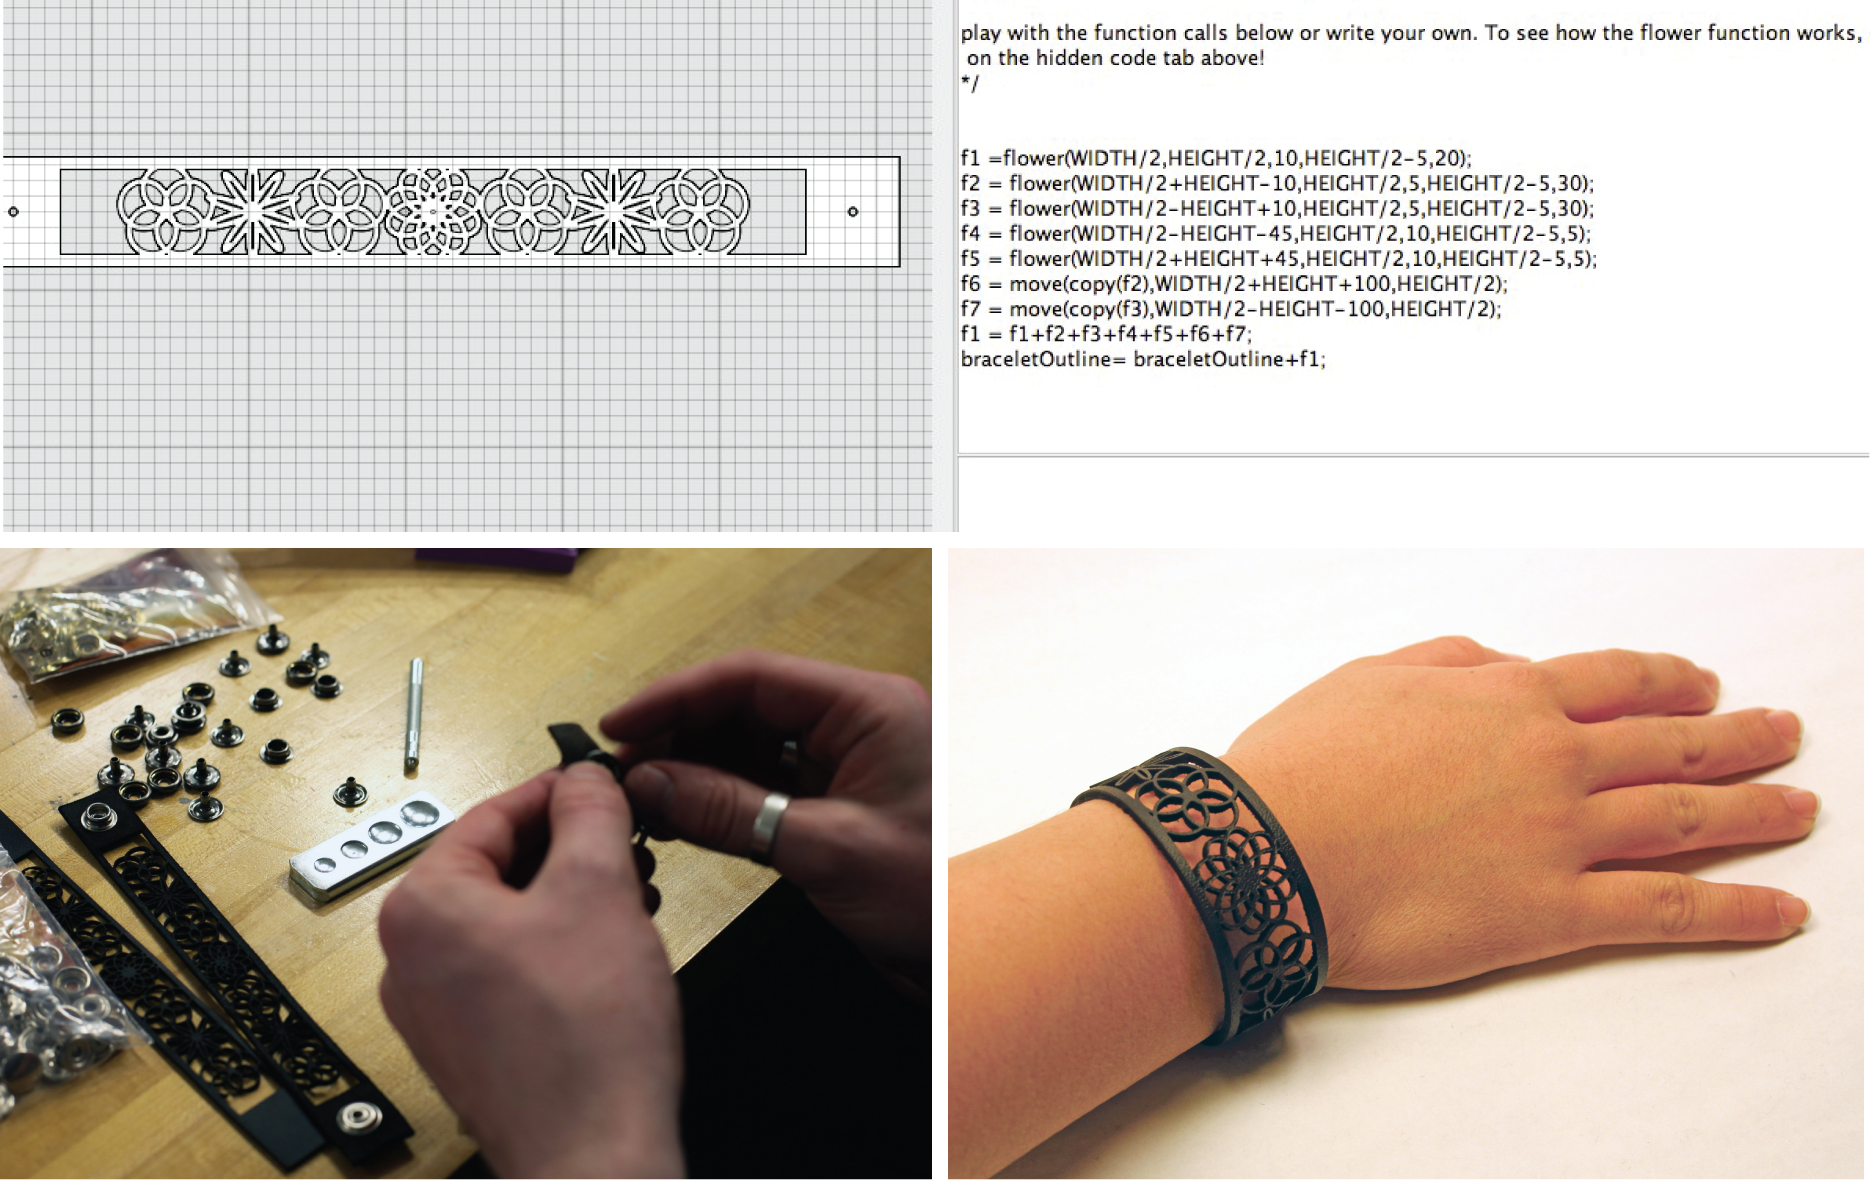
\includegraphics[width=6.5in]{images/dressCode_main.png}
\end{center}


The preliminary work of Codeable Objects and Soft Objects clearly demonstrated that algorithmic craft offers a compelling opportunity for personal, creative expression through programming. My goal following these projects was to address some the limitations present in these preliminarily projects by developing a stand-alone programing environment and design tool. The resulting software, DressCode is a tool developed expressly to support new programmers in open-ended casual computational design for digital fabrication. To evaluate Dress Code, I conducted two separate day long workshops, one with experienced programmers and designers, and one for young people who were new to programming. I also worked with FUSE, an out of school STEAM exploration program to develop a set of online activities using DressCode, which is currently in the preliminary stages of evaluation.	 

\section{Design principles}
Based on the success of the prior fashion workshop, and my continued interest in exploring applications that appeal to women and girls, I decided to focus on computational fashion design and the fabrication of wearable artifacts in the development of DressCode. After reflecting on the potential limitations of this focus however, I decided to develop DressCode as a more open-ended computational design tool that could support the creation of a variety of artifacts, rather than just fashion. To preserve the emphasis on fashion, the majority of the example projects and artifacts I created with DressCode for this thesis were fashion-oriented. The workshops I conducted, as well as the curriculum I helped develop also had an emphasis on fashion or wearable artifacts.

By building my own software, I sought to improve on the preliminary programming libraries in three key areas. First, DressCode contains its own programing language. The DressCode language has a simplified syntax and contains a limited set of textual programming methods, allowing people with little-to-no prior programming experience to working with the language quickly and effectively. Second, the DressCode environment is designed to equally prioritize textual programing and visual design and manipulation. To that end, the software has a two-panel development environment that displays a graphic two-dimensional (2-D) rendering of the user's current design in the first panel, and their code in the second. As a user makes changes to their code, the effects on the design are rendered in the graphic panel. Finally, DressCode contains functionality that is specific to digital fabrication and algorithmic craft. The tool allows for a variety of methods to translate one's design to a tool-paths for fabrication machines. In addition, the API contains programing methods that support the creation of forms and patterns that are suitable for fabrication, with minimal effort on the part of the user.  The goal of designing a software 2-panel programing and design environment, with a specialized programing language and immediate support for digital fabrication was to assist non-programmers in independently making design decisions with programing. In short, I wanted to make it as easy as possible for people to decide on their own desired style or aesthetic, and then realize it by writing their own code. The following section describes the features of the DressCode software in greater detail.

\section{Tool description}
DressCode is a programing and graphical design environment that enables the creation of 2D designs for 2-axis fabrication machines. DressCode is composed both of the application itself, and a custom programing language designed to correspond with the application.

\subsection{Interface Design}
 \begin{center}
\begin{figure}[h!]
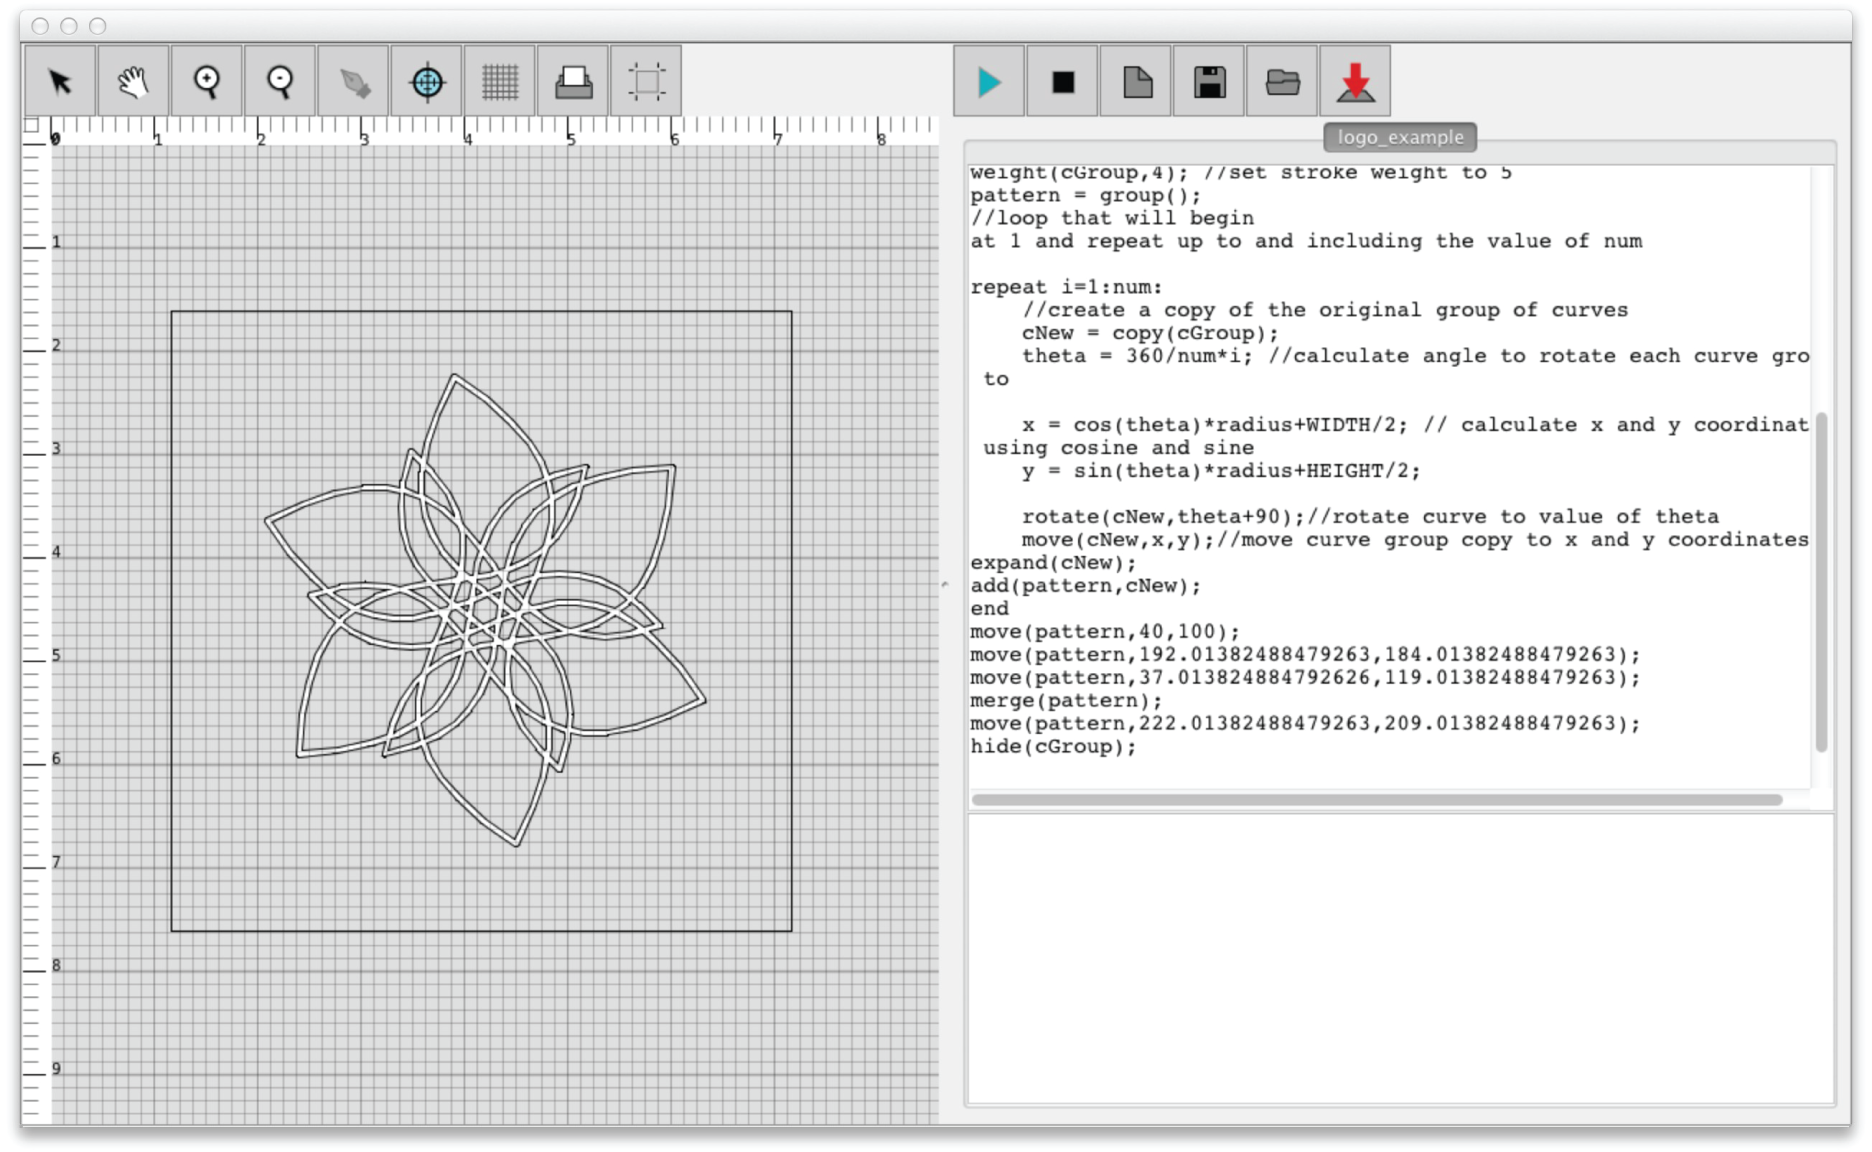
\includegraphics[width=6.5in]{images/dress_code_interface.png}
\caption{The DressCode interface}
\label{fig:dress_code_interface}
\end{figure}
\end{center}

The interface of DressCode is divided into two sections, a design panel and a coding panel. The divider between the two panels can be resized as needed. The coding panel contains a primary window for entering text, an output console for print output and error reporting and a row of buttons on the top. When the play button is pressed, the program in the code window is run and the resulting design is displayed in the design panel. The first version of DressCode ran the code each time the enter key was pressed or a new statement was completed, however we received many requests from our initial user tests for manual control of the run process. The stop button attempts to terminate programs that are taking too long to run.The following three buttons allow for the creation of new programs and the saving and opening of existing programs. The final button opens a dialog that enables the user to select an Scalable Vector Graphics (SVG) file to import into their script (the rationale for this is described in \ref{par:shape_transformation} section below.)

The design panel is primarily composed of the drawing canvas. The drawing canvas has a set of rulers and a grid, along with a black rectangle in the center which serves as the drawing board. The drawing board defines a reference for the coordinate system of the canvas, with the upper left hand corner corresponding to (0,0) in cartesian coordinates. Designs can be drawn on any part of the canvas, including outside the drawing board, however the exported designs file-dimensions will always correspond to the size of the drawing board. The right-most button in the design panel allows for the specification of the units of the project, and the resizing of the drawing board. The print button opens a dialog that allows the user to export their current design in a vector format. I experimented with various vector file formats including DXF, SVG and PDF, however for the time being, I settled on PDFs as they were compatible with the specific fabrication machines I intended to use in my workshops. 

The grid button allows the user to toggle between a grid in the units that correspond to the current units of the project (either millimeters or inches), pixels, or no grid. The target button allows the user to graphically select a set of coordinates and have them appear in the programming window as text, and can be used like an eyedropper for pixel coordinates. The plus and minus magnifying glasses and the hand tool are used to pan and zoom in and out of the screen.  Lastly, the arrow tool allows for design elements to be graphically selected and manipulated. After a design element is moved with the arrow tool, with the corresponding code for the move appears in the programing window. 

  %\begin{center}
%\begin{figure}[h!]
%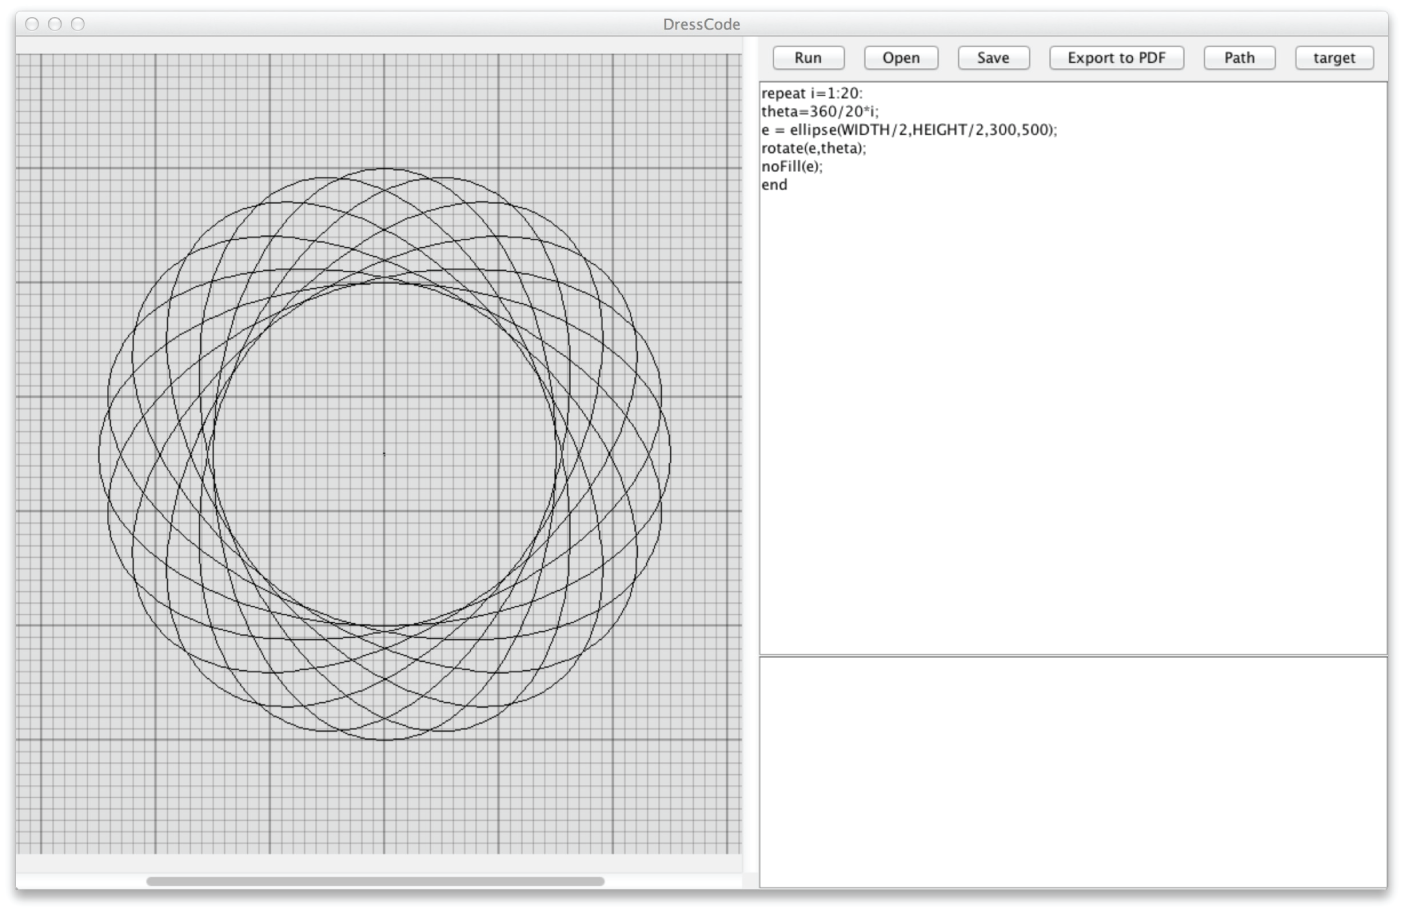
\includegraphics[width=6.5in]{images/early_dress_code.png}
%\caption{The first bare-bones version of DressCode}
%\label{fig:early_dress_code}
%\end{figure}
%\end{center}

\subsection{Programing Language}
The DressCode programing language is interpreted with semantic functionality that is simulated through a Java-based library.  We relied on the ANTLR framework to generate the necessary lexing and parsing methods for the language, and developed the semantic functionality using java and the java openGL (JOGL). When a program is run in DressCode, the raw script is first tokenized and then parsed to generate an abstract syntax tree (AST). During this phase, all user-generated function definitions are stored in memory. If any parsing errors are encountered, they are output to the console as "compiler errors". Assuming the parse is successful, DressCode then walks the resultant AST and attempts to execute the semantic functionality of the program (figure:\ref{fig:interpreter_structure}.) After being executed, the resultant design is rendered on the display panel. Any runtime errors are displayed in the output console. For most programs, this process is instantaneous, however some programs with complex operations require several seconds to be executed. 
  \begin{center}
\begin{figure}[h!]
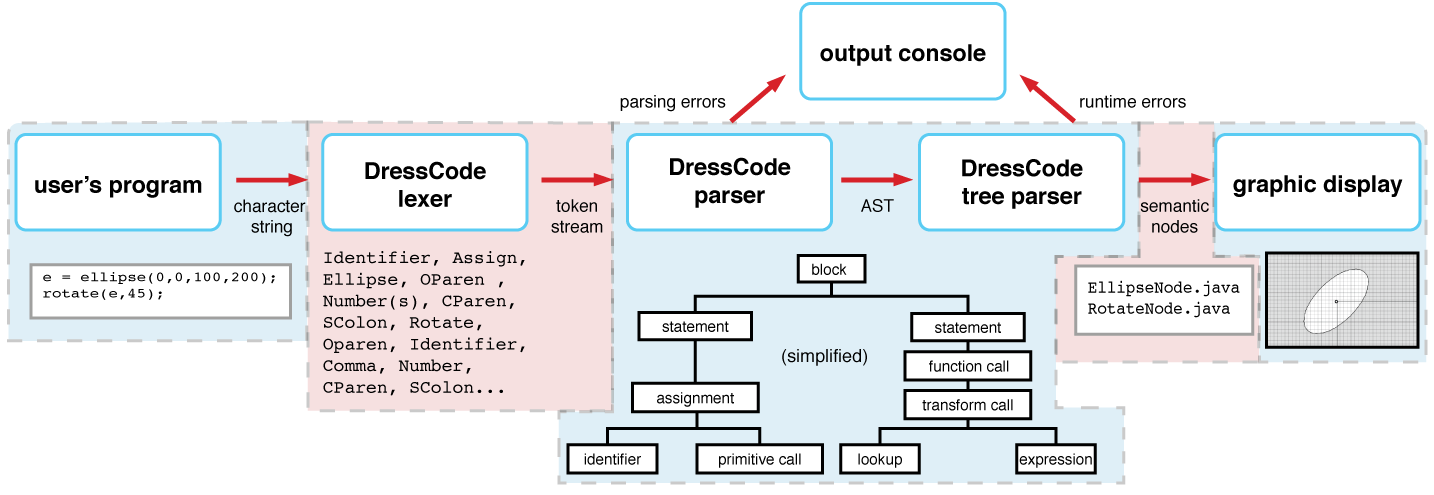
\includegraphics[width=6.5in]{images/interpreter_structure_horz.png}
\caption{Interpreter structure}
\label{fig:interpreter_structure}
\end{figure}
\end{center}
The language is imperative in nature, with statements being executed in the order in which they are read. The exception to this is user defined functions, which may be defined at any point in the program, and called before they are defined. Each statement in DressCode must be terminated by a semicolon. I spent some time experimenting with terminating statements with newlines, similar to whitespace sensitive languages like Python, as I thought this might be more conducive to novice use. Unfortunately, the implementation of selective whitespace recognition is a challenging task to define in a grammar, so while we were able to develop a version of DressCode that recognized statements terminated by a line break, it would have taken significant time to develop this functionality to a level of robustness appropriate for user testing. For the short term, we have opted for a syntax requiring semicolons, however we plan to continue to explore newline statement termination in the future. 

\subsubsection{Language Structure}
Here, I define some of the primary elements of the DressCode syntax and drawing API, and the rationale for their structure. A more thorough language reference is available on the DressCode wiki\cite{DressCodeWiki}.

 DressCode supports number, string, boolean, and drawable datatypes (figure \ref{fig:basic_datatypes}.) The first four of these types are relatively standard in comparison to conventional programing languages. Numbers include integers and floating point values. Strings include any sequence of characters enclosed in double quotations. Booleans have two possible values: true, and false. Drawables are a special type, discussed in detail in the API description below. DressCode also contains a list data structure, which can store multiple kinds of datatypes.
\begin{center}
%\begin{figure}
\begin{lstlisting}
myString = "hello";  //string
myNum = 10.4;  //number
numbermyBool = true;  //boolean
myList = [10,11,false,"world"];  //list with multiple data types
println(myList[3]); //prints world
\end{lstlisting}
%\caption{basic datatypes}
%\label{fig:basic_datatypes}
%\end{figure}
\end{center}

Variable identifiers in DressCode must begin with a letter which followed by 0 or more letters or digits. Variables can be initialized through assignment, or declared and assigned later in the program. All assignment in DressCode is dynamically typed, and variables can be assigned to datatypes that differ from their original assignment at any point. %(figure \ref{fig:variable_assignment}.)

\begin{center}
%\begin{figure}
\begin{lstlisting}
s1 = "hello";
s2 = "world";
s3; //variable without initial assignment

s3 = s1+" "+s2; 
println(s3); //prints hello world

n1 = 2;
n2 = 2.5;
println(n1+n2*10); // returns 27.0
\end{lstlisting}
%\caption{variable assignment.}
%\label{fig:variable_assignment}
%\end{figure}
\end{center}

The  language also contains support for basic expressions, as well as block statements, including conditionals, loops and user-defined functions. For mathematical expressions, standard order of operations is maintained, unless parentheses are introduced. All block statements are signified by a keyword followed by a colon, and terminated with the end keyword which is not followed by a semicolon.Conditionals are defined with the if keyword, and may an optional else clause and  zero or more else if clauses. %(figure: \ref{fig:conditionals}.)

\begin{center}
%\begin{figure}
\begin{lstlisting}
//if statement 
if 5<10:
println("true"); //prints true
end

//if statement with else if and else clause
i=10;
if i<10:
println("less than 10");
else if i==10:
println("equals 10"); //prints equals 10
else:
println("greater than 10");
end
\end{lstlisting}
%\caption{conditional definitions}
%\label{fig:conditionals}
%\end{figure}
\end{center}

There are two possible loop statements: repeat statements and while statements. Repeat statements begin with the repeat keyword and are followed by a the initialization: a variable identifier with a numerical assignment, followed by a colon and the test, a number that determines the point at which the repeat statement will terminate. By default, all repeat statements have an update value of 1, however this can be modified by following the test value with "add" and a 3rd value specifying the update condition. While loops are initialized with the while keyword and followed by a test condition.%(figure: \ref{fig:loops}.) 

\begin{center}
%\begin{figure}
\begin{lstlisting}
//repeat statement
repeat i=0:10:
ellipse(0,i*10,10,10); //draws a vertical row of 10 ellipses
end

//repeat with modified update condition
repeat i=0:10 add 2:
println(i); //will print 0,2,4,6,8
end

//while statement
c=0;
while c < WIDTH:
ellipse(c,10,20);
c = c+20;
end
//draws a row of ellipses that span the width of the canvas
\end{lstlisting}
%\caption{loop definitions}
%\label{fig:loops}
%\end{figure}
\end{center}

Finally, custom functions are defined with the def keyword, followed by an identifier and a set of parentheses containing 0 or more arguments separated by commas. The function block is terminated with the end keyword like all other block statements. Just like general assignments, functions arguments are dynamically typed. Functions, loops and conditionals all have their own scope and will prioritize identifiers based on that, however if they cannot locate an identifier within their own scope, they will look for it in the level above.
\begin{center}
%\begin{figure}
\begin{lstlisting}
//basic function defintion
def foo(a,b,c):
println(a+b+c);
end

//function call
foo(1,2,3);  //prints 6

//function with return statement
def bar(a,b,c):
return(a*b*c);
end

result = bar(4,5,6)); 
println(result);//prints 120
\end{lstlisting}
%\caption{loop definitions}
%\label{fig:loops}
%\end{figure}
\end{center}

\subsubsection{Drawing API}
 The API is organized around the creation and transformation of 2D shape primitives. By duplicating and manipulating these primitives in a structured manner, it is possible to generate complex and interesting designs from simple forms. The API is composed of three primary main categories, divided by functionality: shape primitives, shape transforms, shape booleans, math operations and property access. A selection of the primary methods from each of these categories is detailed in figure \ref{fig:api_table}. 

  \begin{center}
\begin{figure}[h!]
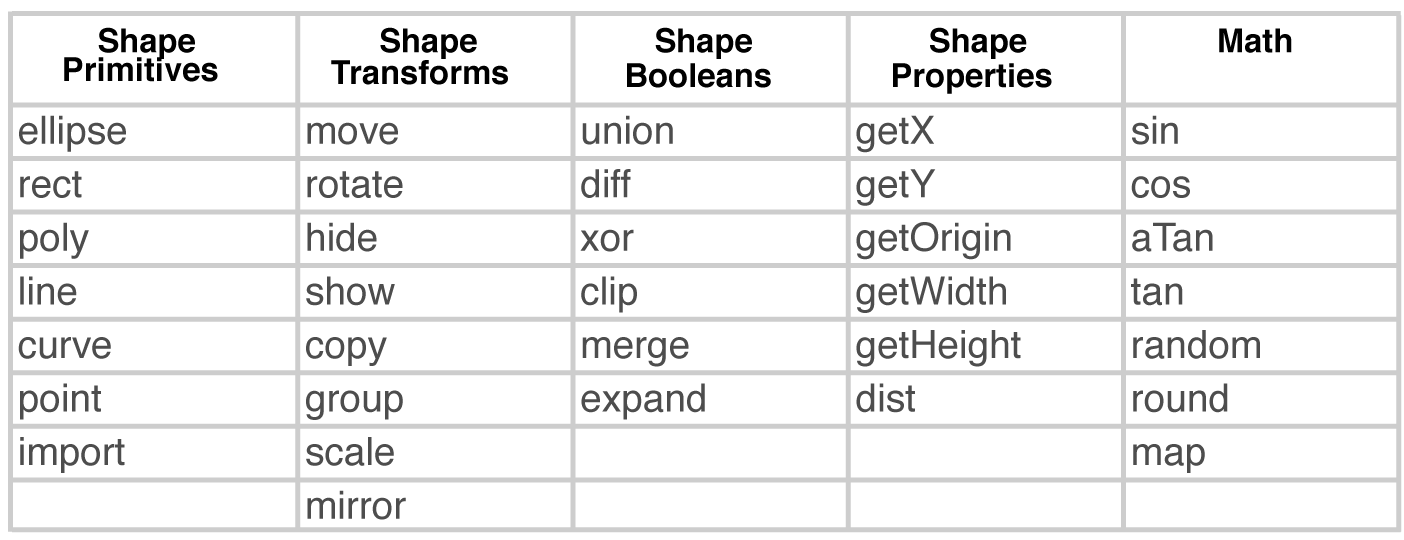
\includegraphics[width=6.5in]{images/api_table.png}
\caption{A selection of methods from the DressCode API}
\label{fig:api_table}
\end{figure}
\end{center}
\paragraph{Shape Primitives:}
DressCode shape primitives currently serve as the primary means of drawing (figure: \ref{fig:shape_primitives}.) The simplest primitive is a point, initialized two numerical parameters that denote the x and y coordinates. All closed-shape primitive methods (ellipses, rectangles and polygons) require an argument of either two x,y coordinates, or a point. This coordinate defines the origin of the shape and determines where  the shape will be drawn on the canvas. Ellipses and rectangles have an additional two optional parameters which specify width and height. If only two arguments are provided, the ellipse or rectangle will be drawn with a default width and height; if three arguments are given, the width and height will be the same. Polygons also have two optional parameters following the x and y origin coordinates, however they specify number of sides and length of each side, rather than width and height. Lines can be initialized either as four numerical values, specifying start and end x and y coordinates, two points, or as a vector, with a origin point,  a magnitude, and a heading in degrees. Curves are defined by a set of four points or eight coordinates, which determine the start, first control point, second control point and end point of a 4-point bezier curve. One other method of primitive generation was added in at the request of some of our early users: vector paths stored in Scalable Vector Graphics (SVG) format can be imported and drawn in the DressCode environment, and used in conjunction with primitive transformation and boolean methods.  

 \begin{center}
\begin{figure}[h!]
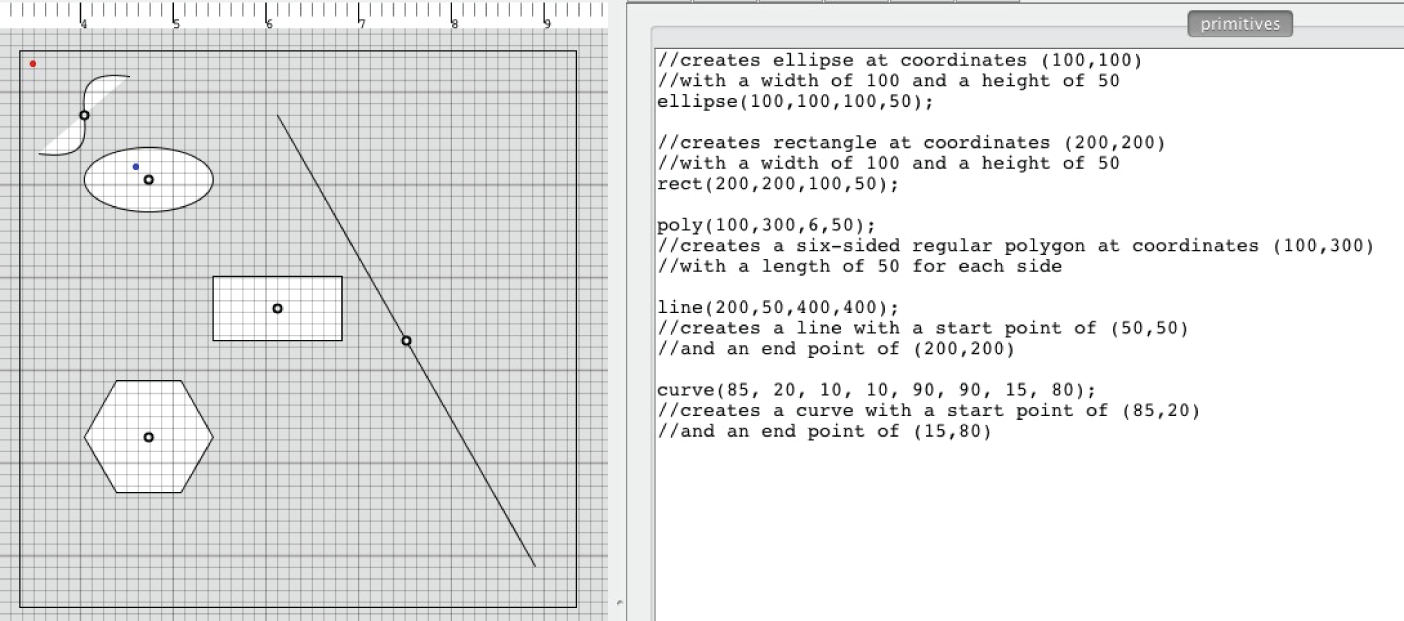
\includegraphics[width=6.5in]{images/primitives.png}
\caption{DressCode shape primitives with visible origins}
\label{fig:shape_primitives}
\end{figure}
\end{center} 

\paragraph{Shape Transformations:} \label{par:shape_transformation}
There is no required "draw" method for DressCode, as there are in many other graphics APIs, Instead all primitives are automatically drawn in the display panel in the order of their initialization, once the program has been run. In Soft Objects and Codeable Objects, when we required users to manually call draw method for any and all shapes in their program, they often forgot, and then had difficulty determining the reason why parts of their designs were not visible. 

Each shape primitive method returns an instance of the primitive it creates. A programmer can either create shapes with no reference as in figure \ref{fig:shape_primitives}, or they can assign them to an identifier at initialization, allowing them to reference and modify the shape later in the program. The shape transformation methods allow for a range of modifications to a shape, by passing a reference to the primitive the first argument, followed by different parameters for the modification, depending on the method (figure: \ref{fig:transformation}.) We began with a basic set of transformations, including move, rotate, methods that allowed for the modification of the stroke weight and color of the shape, and a hide method that prevented a primitive from being drawn. Based on our early user testing however, we gradually added in additional methods, based on what people wanted to do with their designs. This included a moveBy method, scale and mirroring functionality, a copy method, and an addition to the rotate method which allowed a shape to be rotated around a point other than its origin. 

 \begin{center}
\begin{figure}[h!]
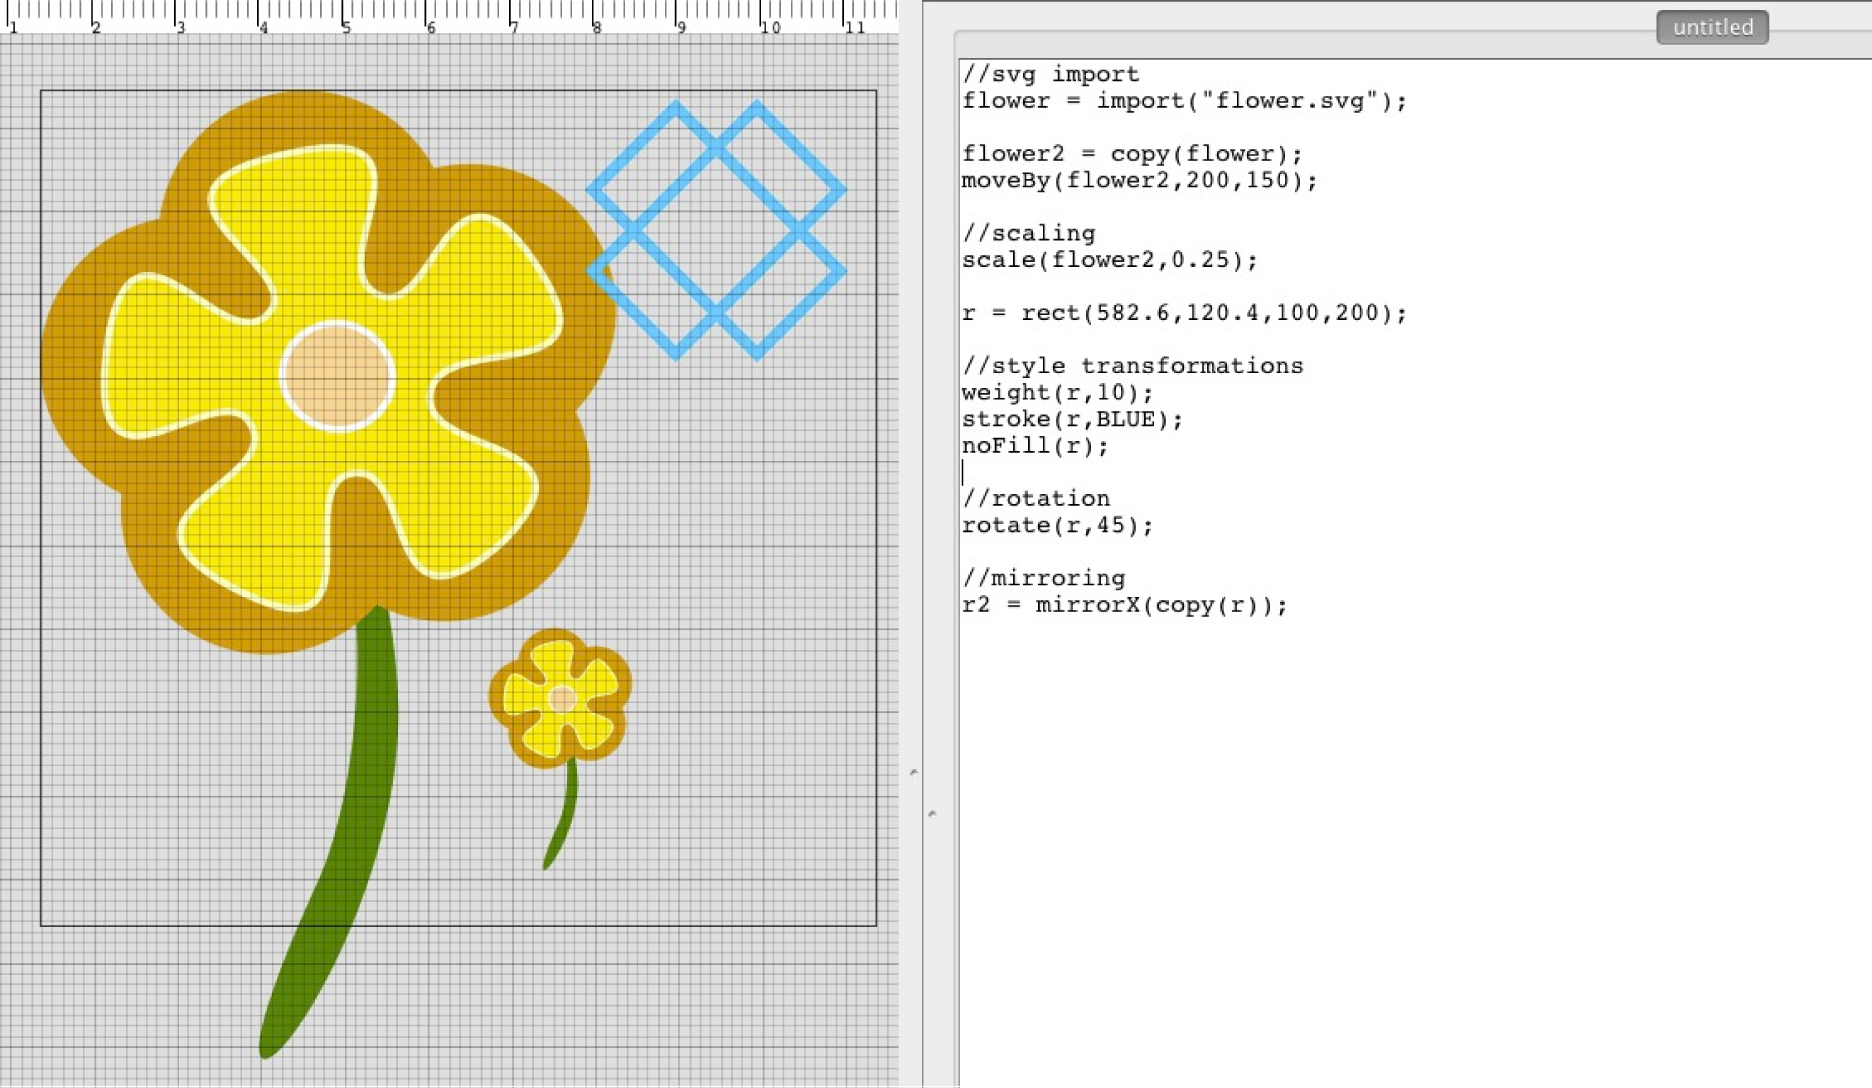
\includegraphics[width=6.5in]{images/transformation.png}
\caption{SVG import and sample of transformation methods}
\label{fig:transformation}
\end{figure}
\end{center} 

DressCode primitives can also be programmatically "grouped". Grouping provides an organizational structure for more complex configurations of primitives allows for the automatic transformations to multiple shapes. Groups have their own origin, which is used as the reference point for all move, rotation and scale methods applied to the group (figure: \ref{fig:grouping}.) For example, a collection of ellipses that is grouped and then moved to the center of the canvas would move the origin of the group to the center, and all the ellipses relative to the new origin. The origin of a group is automatically calculated as the centroid of all of the objects in the group and updated each time a primitive is added or removed. Groups are treated similarly to lists in that individual objects can be accessed and manipulated by via their index. Originally, primitives within a group were transformed relative to the origin of the group, however this caused confusion among many of our initial users. Each individual primitive is now translated according to the coordinate system of the canvas, regardless of whether it is in a group. 

 \begin{center}
\begin{figure}[h!]
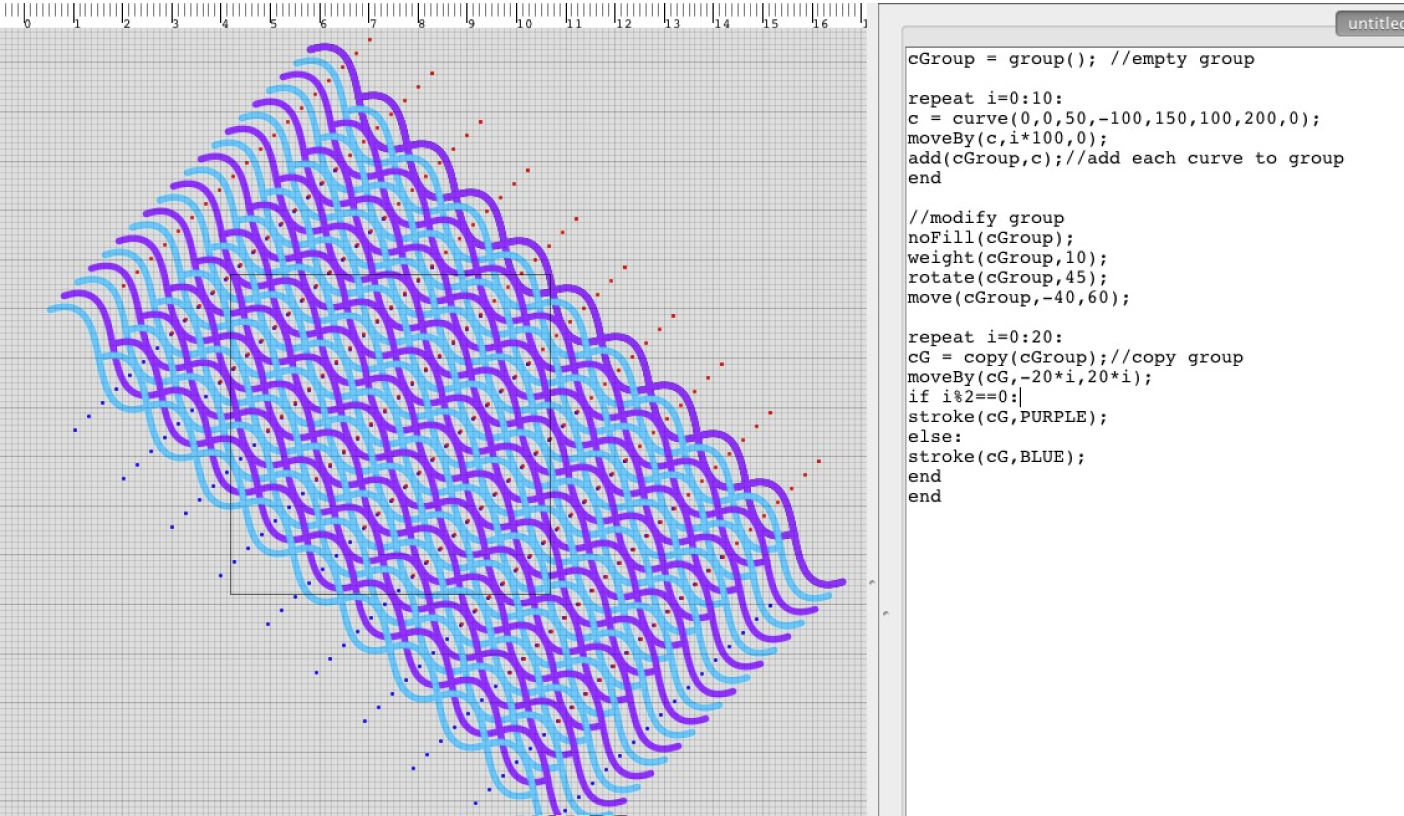
\includegraphics[width=6.5in]{images/grouping.png}
\caption{Grouping with transformation and repeat statements}
\label{fig:grouping}
\end{figure}
\end{center} 

\paragraph{Polygon Booleans:}
DressCode also features a subset of transformation methods for polygon boolean operations (figure: \ref{fig:boolean}.) The union, difference, exclusive or and intersection methods accept two primitives as arguments and return the corresponding shape, or group of shapes, depending on the operation. In addition, the merge method performs a union on all objects within a group and returns a single primitive. The expand method converts an object's stroke to a filled polygon with dimensions that match the weight of the stroke. The boolean methods were added for multiple reasons. Polygon boolean operations play an important role in CAD design for fabrication, because they allow for the creation of vector paths that appropriate for subtractive manufacturing processes. In particular, the merge method can function as a catch-all method for preparing designs for fabrication, and the expand method is useful for converting line drawings to paths that will retain their appearance when cut. In prior workshops, we relied on illustrator to prepare file paths for manufacturing, which was difficult, time-consuming and a hindrance to the computational design process. By integrating boolean operations as a part of the programming language in DressCode, it not only prevents users from having to rely on multiple software tools to design, but allows booleans to be used in a computational context, facilitating the creation of a whole new range of forms with simple primitives. 

Both the syntax and functionality of the boolean operations have been modified significantly since the first version of DressCode. In early versions, the majority of the booleans were expressed through mathematical notation, rather than with built in functions (e.g. ellipse1 + ellipse2 would perform a union). After some of our early user testing however, we depreciated this syntax, because many testers felt that mathematical notation was not intuitive beyond the union and difference operations. In addition, the mathematical notation required that all booleans be set equal to an identifier  (e.g. ellipse1 + ellipse2 = e3), in order to evaluate as a valid statement. The new method syntax still returns a resulting boolean, but can also be called without a corresponding assignment statement. Semantically, we originally had the boolean statements operate in a destructive manner as is the case in many graphic drawing programs; union(ellipse1, ellipse2) would destroy the original two ellipses and set the identifier ellipse1 equal to the resulting boolean. This was confusing however, because in a imperative program, the programmer could still reference the destroyed ellipse2. What we opted for instead, was a non-destructive boolean method wherein union(ellipse1,ellipse2) would return a third shape, which would automatically be drawn on the screen, and could be assigned to an identifier as needed. The original ellipse1 and ellipse2 would be hidden, but could both still be referenced without conflict, and could be revealed again on the canvas with the show() method. 

 \begin{center}
\begin{figure}[h!]
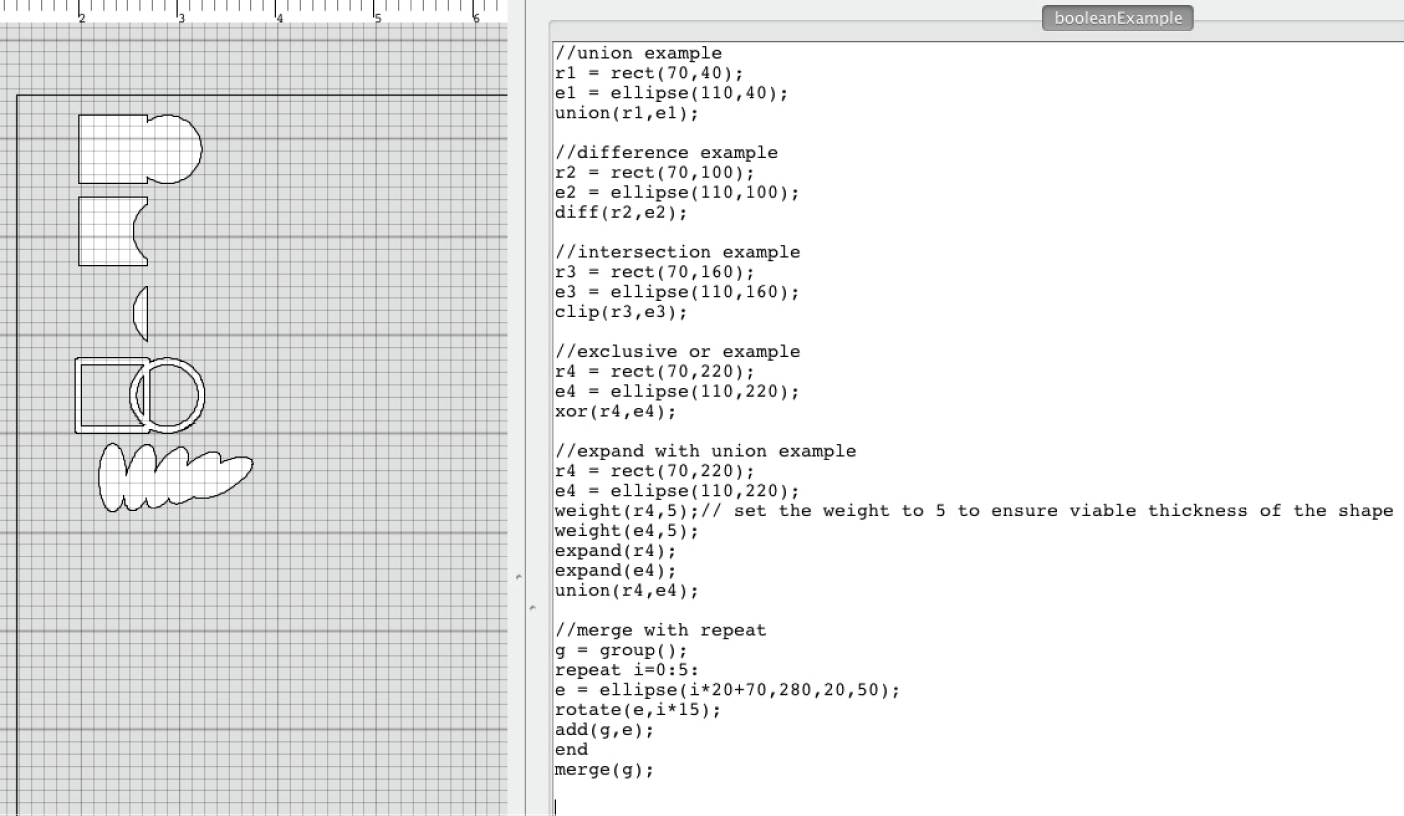
\includegraphics[width=6.5in]{images/boolean.png}
\caption{Polygon boolean operations}
\label{fig:boolean}
\end{figure}
\end{center} 
\paragraph{Additional Methods:}
Aside from methods for shape generation and transformation, DressCode features a set of getter methods that return information about a shape primitive, including its location, origin point, width and height, as well as a method to determine the Euclidean distance between two objects. There are also a set of methods that enable more advanced mathematical operations, including trigonometric functions, mapping, rounding and random number generation. The random method posses an interesting questions for implantation, as it generates different numbers each time a a program is run. This can be a useful design feature, allowing for the generation of numerous patterns with random variations. Figure \ref{fig:random_symmetry} demonstrates variations of an algorithm that produces randomly symmetrical stripe patterns.  It can also become problematic however, when the user wishes to keep the same randomly generated number for each interpretation of their program.  Finally, we recently added a set of methods that allow the specification of numerical values in inches, centimeters and millimeters, or in the current units of the drawing board. These methods are helpful when sizing and transforming primitives to real world measurements rather than pixel values.  

\paragraph{Constants:}
DressCode has a small set of constants to assist with design. WIDTH and HEIGHT correspond to the width and height of the current drawing board. PI corresponds to the numerical Pi value. Lastly, there are a set of color constants; RED, GREEN, BLUE, PURPLE, PINK, etc., that can be used to define the color of objects with fill and stroke methods. Custom colors can also be specified with 0-255 RGB values. 

 \begin{center}
\begin{figure}[h!]
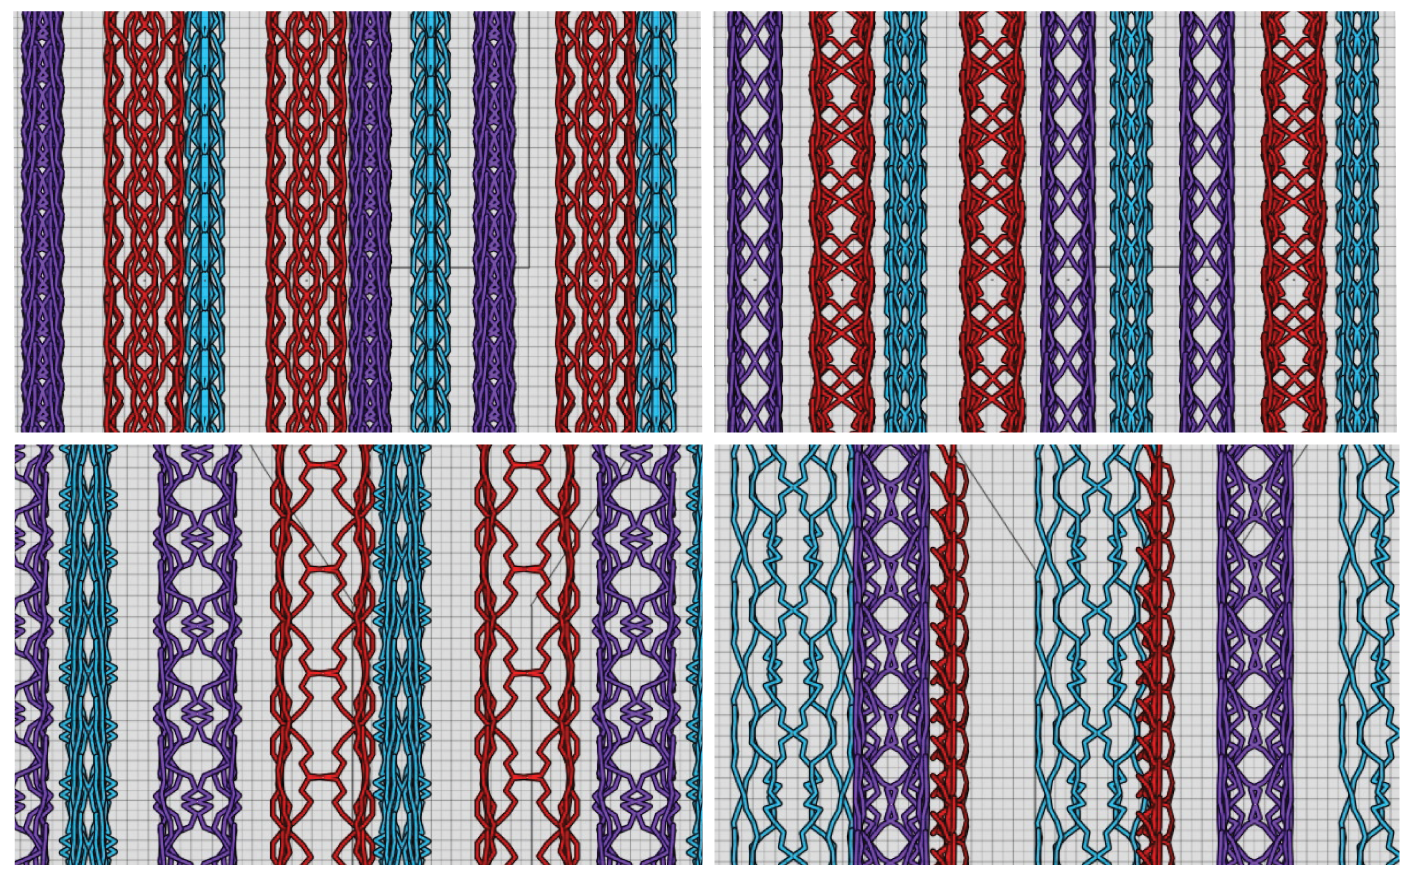
\includegraphics[width=6.5in]{images/random_symmetry.png}
\caption{Stripe pattern variations using the DressCode random method }
\label{fig:random_symmetry}
\end{figure}
\end{center}

\section{Fabrication and Crafting Process}
Similar to the prior tools described in this thesis  once a design is exported from DressCode, it can be imported to the control software of any 2-axis fabrication machine and fabricated into a set of parts.Depending on the material and fabrication process, a variety of end products are possible. In the process of protopying DressCode, I experimented several different fabrication machines, crafting techniques and artifacts. I tested DressCode primarily with the laser-cutter, however I also used it with more accessible machines including low-cost craft vinyl cutters and inkjet printers. I also examined sending DressCode files to online fabrication services such as Shapeways and SpoonFlower, to produce 3D-printed jewelry and larger inkjet printed garments.  I tested the resultant pieces from these fabrication processes with different crafting techniques that ranged in difficulty. Highly accessible techniques included making artifacts that required basic paper-folding or iron on appliqu�s for clothing. More difficult techniques included sewing garments, screen printing onto fabric, and jewelry making. There was frequently correlation between how easy a craft was to create, and how well it corresponded with the DressCode design process, indicating that for more sophisticated crafting processes like sewing, more advanced organizational functionality might be required for the DressCode software. 

To provide some support in the crafting process for independent users, my undergraduate research assistants and I created a set of example templates in DressCode that are directed towards specific end projects and fabrication machines (figure: \ref{fig:dresscode_examples}). We also began documenting some of the crafting techniques required to complete these projects online \cite{thesis_website}. Mainly though, I relied on in-workshop instruction or curriculum development to assist people in using DressCode to complete finished artifacts.

 \begin{center}
\begin{figure}[h!]
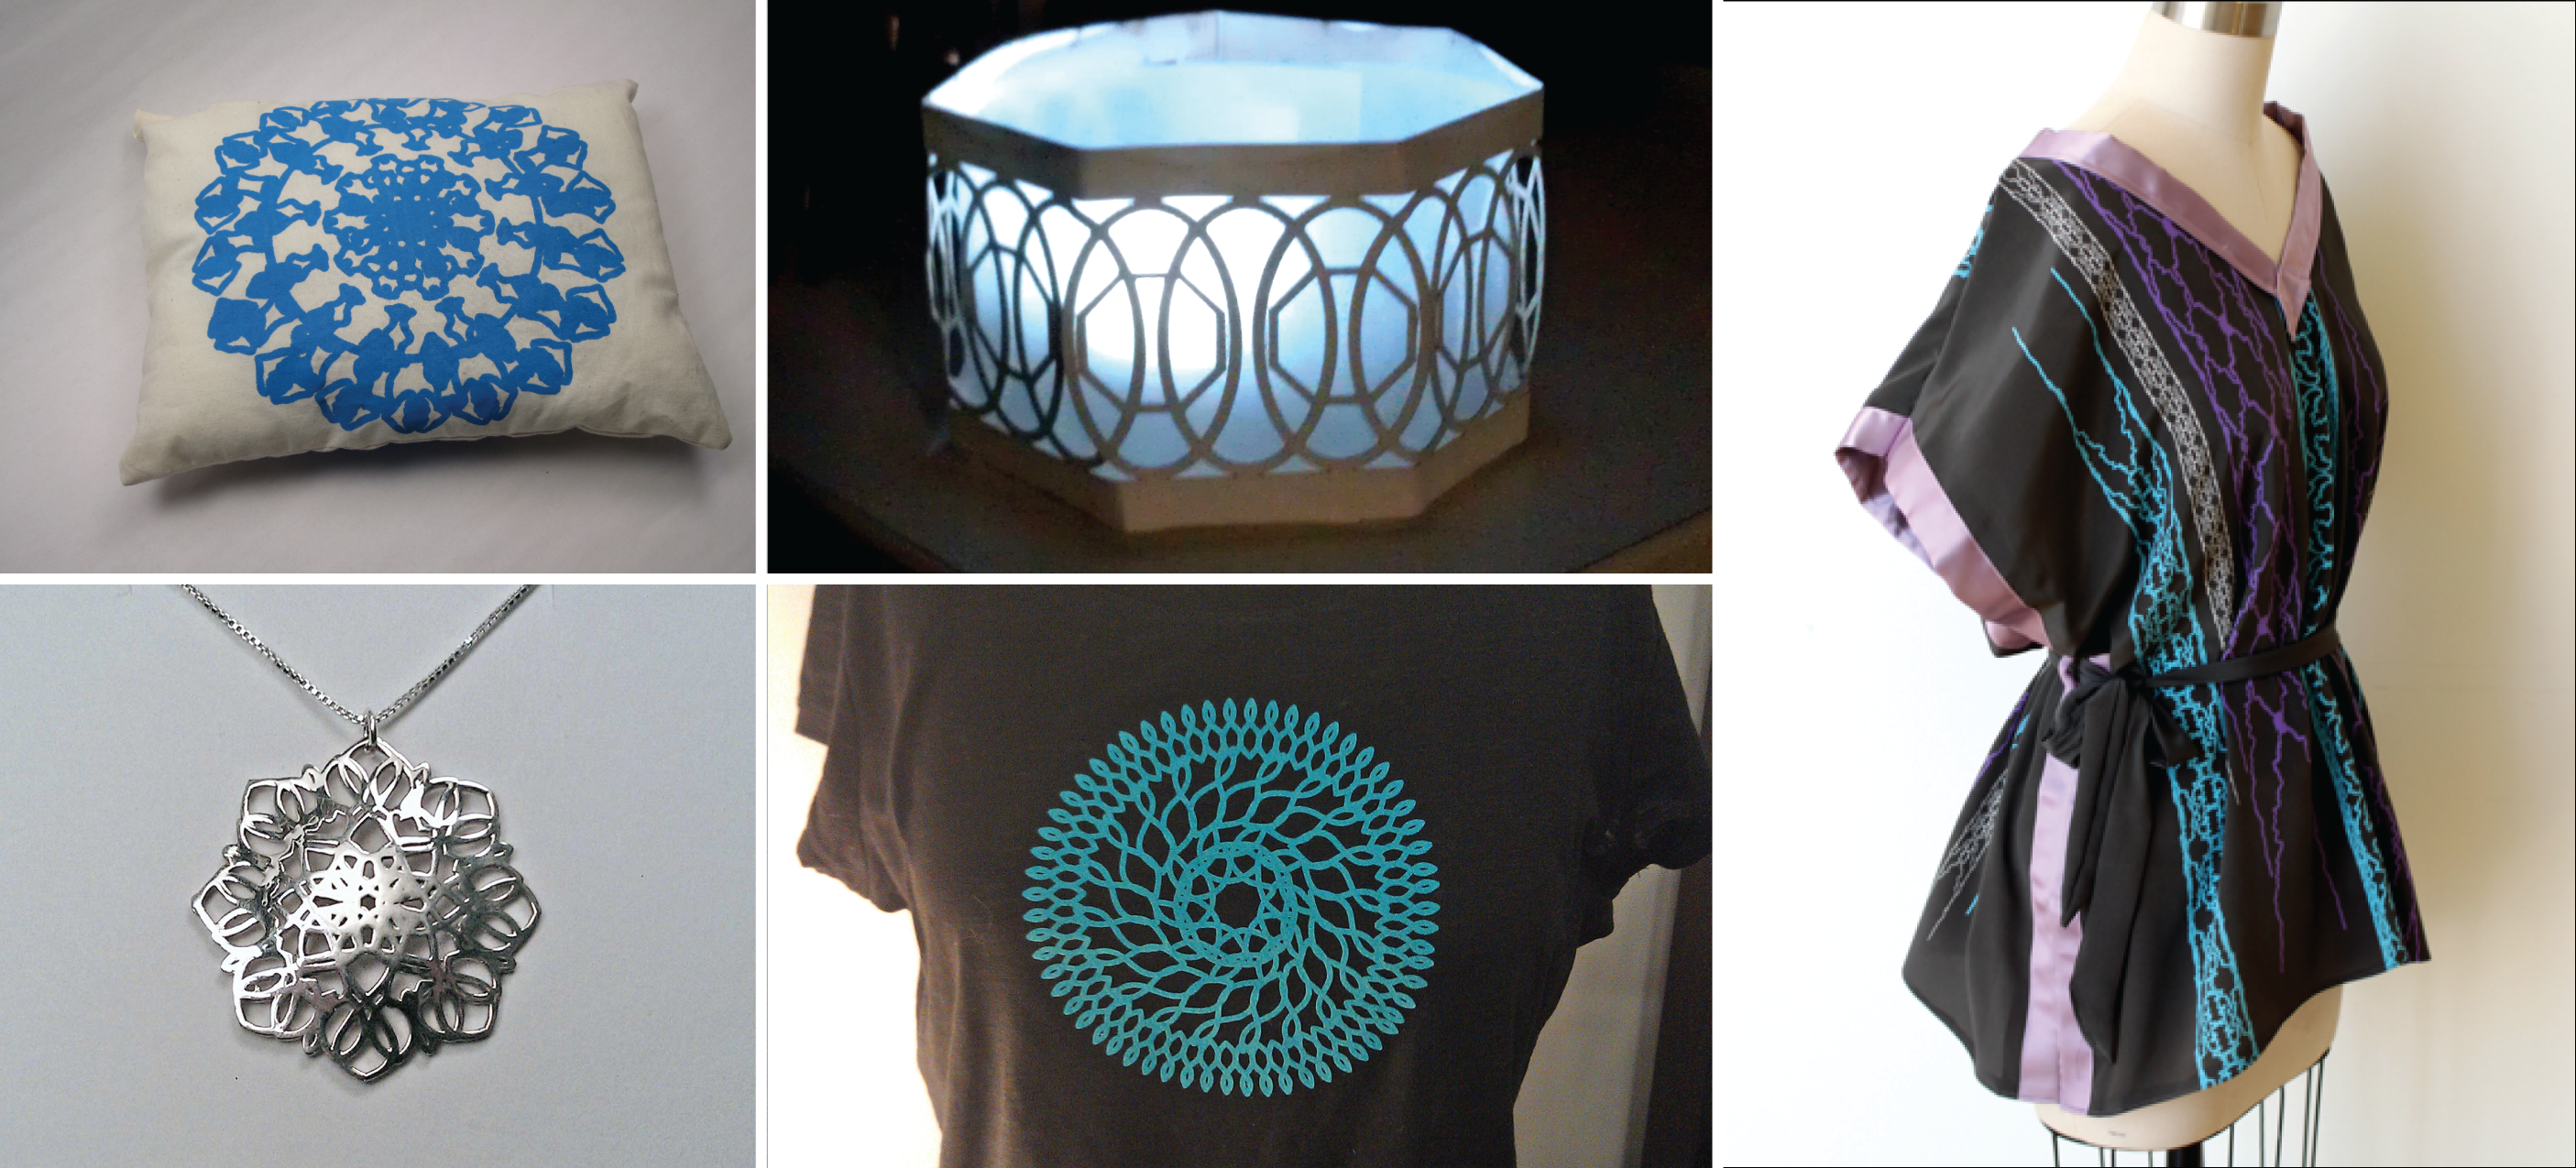
\includegraphics[width=\columnwidth]{images/dresscode_examples.png}
\caption{Several example artifacts created with DressCode Designs (clockwise from top left: vinyl-cut screen printed pillow, vinyl-cut tea light, ink-jet printed silk caftan, laser-cut iron-on tshirt, 3d printed silver pendant) }
\label{fig:dresscode_examples}
\end{figure}
\end{center}


\section{Workshops}
We informally tested DressCode with members of the FUSE development team, and by the staff at Dream Yard, an after school STEM education space in the Bronx. Following these tests, and a period of additional development, DressCode was evaluated during two separate day long workshops at the MIT Media lab. The first workshop was conducted among experienced designers, artists and programmers, who were selected individually from MIT, Harvard and the Cambridge community. The second workshop was conducted among ten young adults selected from youth organizations in Cambridge and art and craft workshop mailing-lists at MIT.Both workshops used DressCode to create laser-cut leather crafts.

\subsection{Expert Workshop}
The expert workshop was comprised of eight participants between the ages of  19 to 33. Five of the eight participants were female and three were male, and all had prior experience in programming. 75\% of the participants indicated a strong prior interest in design, and 50\% enjoyed crafting. All participants had formal training at a college level in either art, design or computer science 

The expert workshop was deliberately open and informal. We began the workshop with an open 30 minute discussion on the connections and intersections between design, arts and crafts and programming. Following this discussion the, participants were given a 45 minute general tutorial on the basics of the DressCode environment and programming language, after which participants were given access to the DressCode online code reference and a physical handout with quick references for some of the key methods. We also provided with a leather bracelet template and several example programs that generated different patterns for the template as  examples. Participants were given the option to design within the template or rely on modifying these examples, but were also free to create whatever they wanted.  Following the programing tutorial, participants were shown the basic fabrication process, and introduced to the materials, consisting of several varieties and colors of leather. Participants then had 3-4 hours to design their piece. As they completed their designs, they were taken in groups to the shop to fabricate their parts and then given access to craft tools and a variety of fasteners (snaps, rivets and jewelry connectors) to convert them into finished artifacts.

\begin{center}
\begin{figure}[h!]
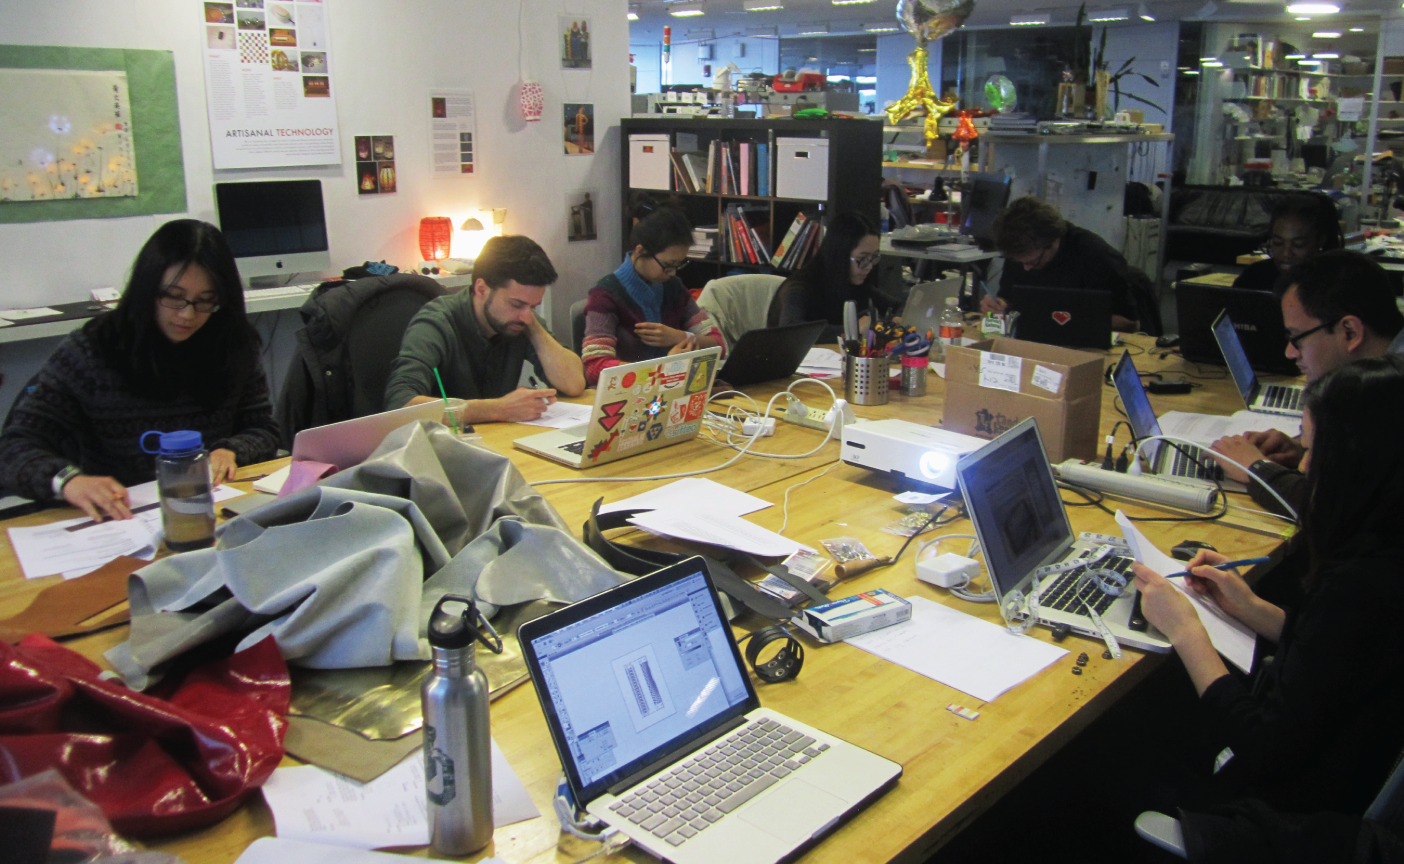
\includegraphics[width=\columnwidth]{images/adult_design_time.png}
\caption{The expert workshop}
\label{fig:adult_design_time}
\end{figure}
\end{center}

\subsection{Youth Workshop}
The youth workshop was conducted among ten young adults, aged 15-17, 20\% male and 80\% female. Five of the youth participants were participants in the Teach to Learn, Learn to Teach program in Boston \todo{cite program and find a description}. Of those surveyed three participants had prior experience with Scratch, and two had worked with the Arduino programing environment in a prior Media Lab workshop.  All of the participants said they had some prior experience in art, design, or craft.  Prior to the workshop, 60\% of the participants indicated that they did not feel comfortable programing on their own, however the majority indicated that they were interested in learning more about the process. 

The youth workshop was more structured than the expert workshop with the goal of helping to familiarize participants with the possibilities and affordances of computational design and fabrication. We began by passing out three colors of post-its for the categories of of art and craft, design and programming. We then held a 5 minute brainstorm where we asked each participant to write down people, tools, ideas and projects the associated each category on the respective colored post-it. After, we collected the post its, and put them up on a board in related clusters, and used the resulting associations to instigate 30 minute discussion on the participants ideas about the connections between the three domains.  We ended the discussion by talking about some of the possible craft applications of computational design, and began the introduction to DressCode.

\begin{center}
\begin{figure}[h!]
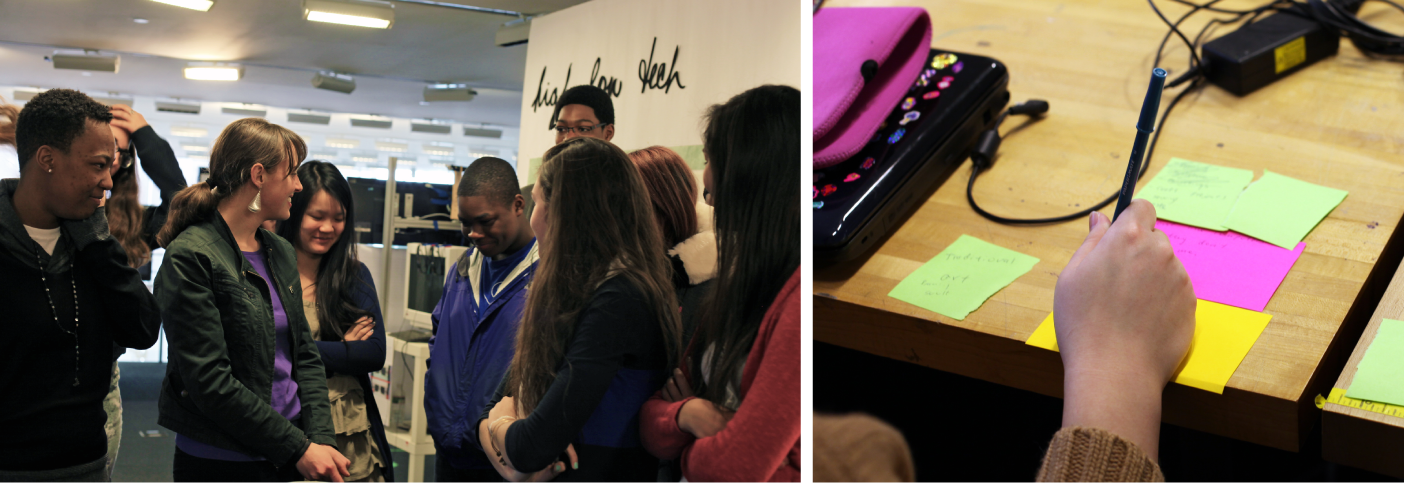
\includegraphics[width=\columnwidth]{images/youth_brainstorm.png}
\caption{The youth brainstorm and discussion}
\label{fig:youth_brainstorm}
\end{figure}
\end{center}

All of the design work in the youth workshop was structured around the concept of radial symmetry. I chose radial symmetry because it is a relatively easy pattern express mathematically, it serves as an excellent motivation for using a loop, and it is a pattern that is commonly found in nature, making it possible to generate designs that are floral,biological or organic in appearance. In addition, radially symmetric forms are often aesthetically appealing to people.  To begin, I explained the concept of DressCode and then spent 20 minutes leading the group, step by step through the process of creating a basic algorithm that used a repeat loop to create and rotate a number of ellipses around a central point (figure: \ref{fig:starting_algorithm}.) After every participant had successfully created their version of the algorithm, I showed them how they could use the same algorithm to create different designs by changing the number of iterations of the loop, the type of shape that was drawn, and the width and height of the shape. Participants then had 15 minutes to experiment with different parameters, and produce different designs, followed by a group show and tell session (figure: \ref{fig:show_and_tell}.) 

\begin{center}
\begin{figure}[h!]
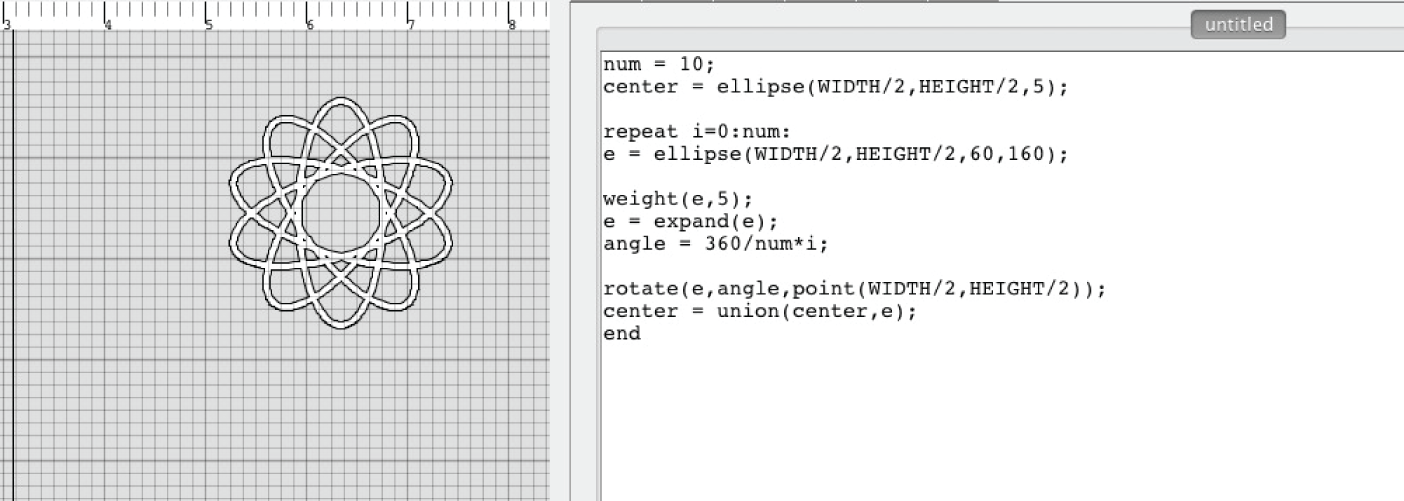
\includegraphics[width=\columnwidth]{images/first_algorithm.png}
\caption{The first algorithm learned by the youth participants}
\label{fig:starting_algorithm}
\end{figure}
\end{center}

\begin{center}
\begin{figure}[h!]
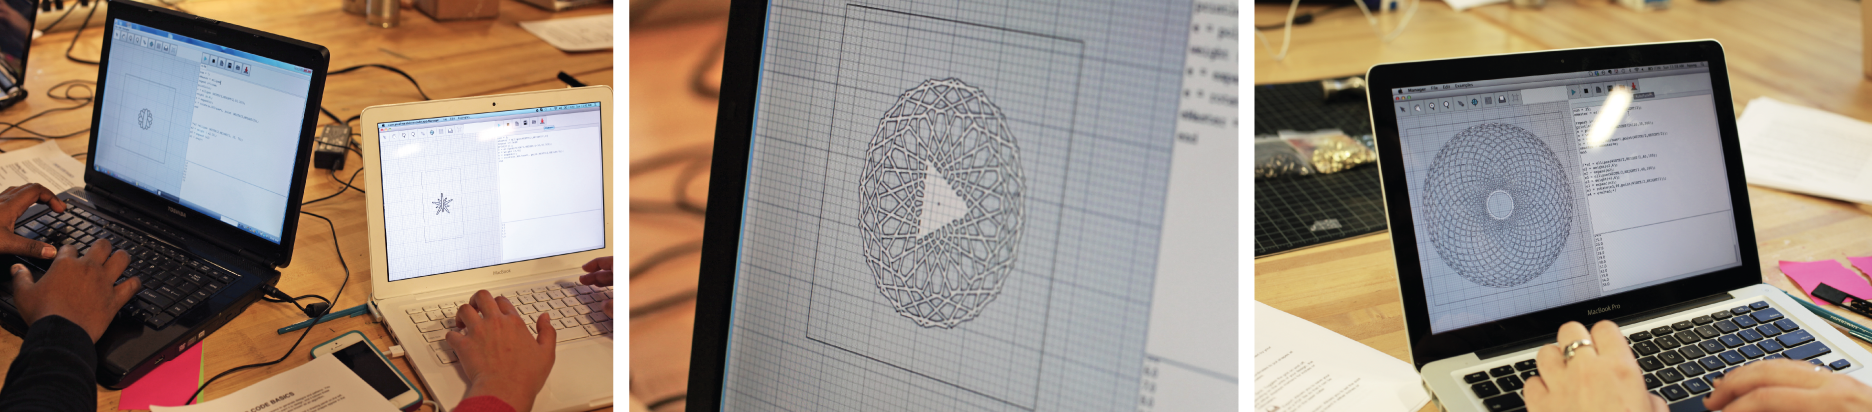
\includegraphics[width=\columnwidth]{images/show_and_tell.png}
\caption{Some example variations on the first activity}
\label{fig:show_and_tell}
\end{figure}
\end{center}

Next, the participants were provided with example programs that contained a bracelet template. The example programs featured a pre-written function that duplicated the algorithm they had written in the previous activity, with arguments corresponding to same values they were manipulating before. Participants were then given time to use the function to make multiple elements of the original radial pattern with different parameters. A second tab in the example program revealed the code for the radial function, which they could modify if they desired. The example template was constrained so that the dimensions of the bracelet would automatically correspond to the size of the drawing board. By measuring their wrist and resizing the drawing board, they could generate a bracelet of the correct size, and maintain their original design (figure: \ref{fig:bracelet_template}.)

\begin{center}
\begin{figure}[h!]
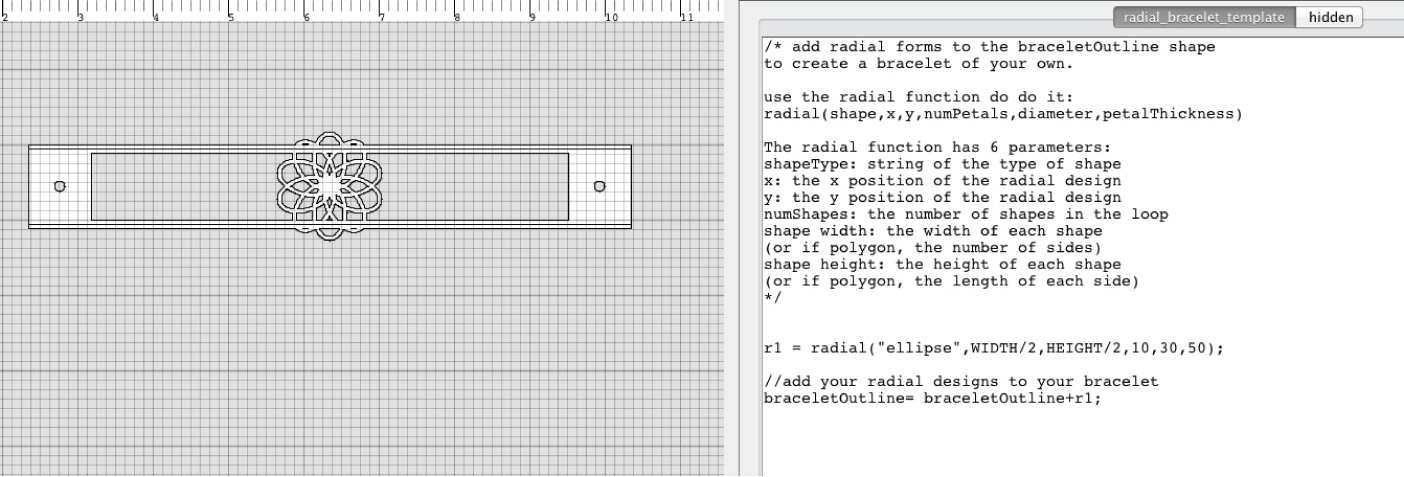
\includegraphics[width=\columnwidth]{images/bracelet_template.png}
\caption{The bracelet template with one instance of the radial function being called}
\label{fig:bracelet_template}
\end{figure}
\end{center}

Participants were given approximately two hours of free design time. When they had settled on a final design, they first printed out a paper copy and ensured that it fit their wrist. Following that, they selected their material and were taken in groups to the laser cutter where they cut their piece. Afterwards, they were shown how to attach the fasteners to the bracelet, and provided with additional handcrafting tools that allowed them to further alter the piece by hand. 

\section{Results}
\subsection{Expert Results}
All but one participant in the expert workshop indicated that they were able to successfully able to complete a finished product. The types of end products varied.  While most participants produced leather cuffs, people also created finger puppets, earrings and a belt using the software. Many participants also mixed materials and techniques and created There was a high degree of variation in the algorithms used to create the finished products. Several participants relied exclusively on the radial symmetry algorithm, but others created patterns with computationally ordered curves, rectangles and lines in different arrangements.  The participant who created the leather belt designed the pattern so that it demonstrated the evolution of the algorithm that comprised it; as the individual patterns progress across the length of the belt, they grow in complexity. Because of the high degree in variation among approaches and end products, conducting the expert workshop was difficult. Many of the participants began with design goals that were at odds with the affordances of DressCode, such as creating representational characters in the case of the finger puppet example, or creating organic, irregular forms.  In addition, several of the end projects required instructor intervention to ensure they were suitable for fabrication. Overall, the expert workshop produced a promising set of results and demonstrated the limitations and benefits of using DressCode across a broad range of design approaches. The expert participants also provided feedback on specific features to incorporate into future versions of the DressCode software. The random method and unit conversion methods were added directly following the workshop based on participant suggestion.

\begin{center}
\begin{figure}[h!]
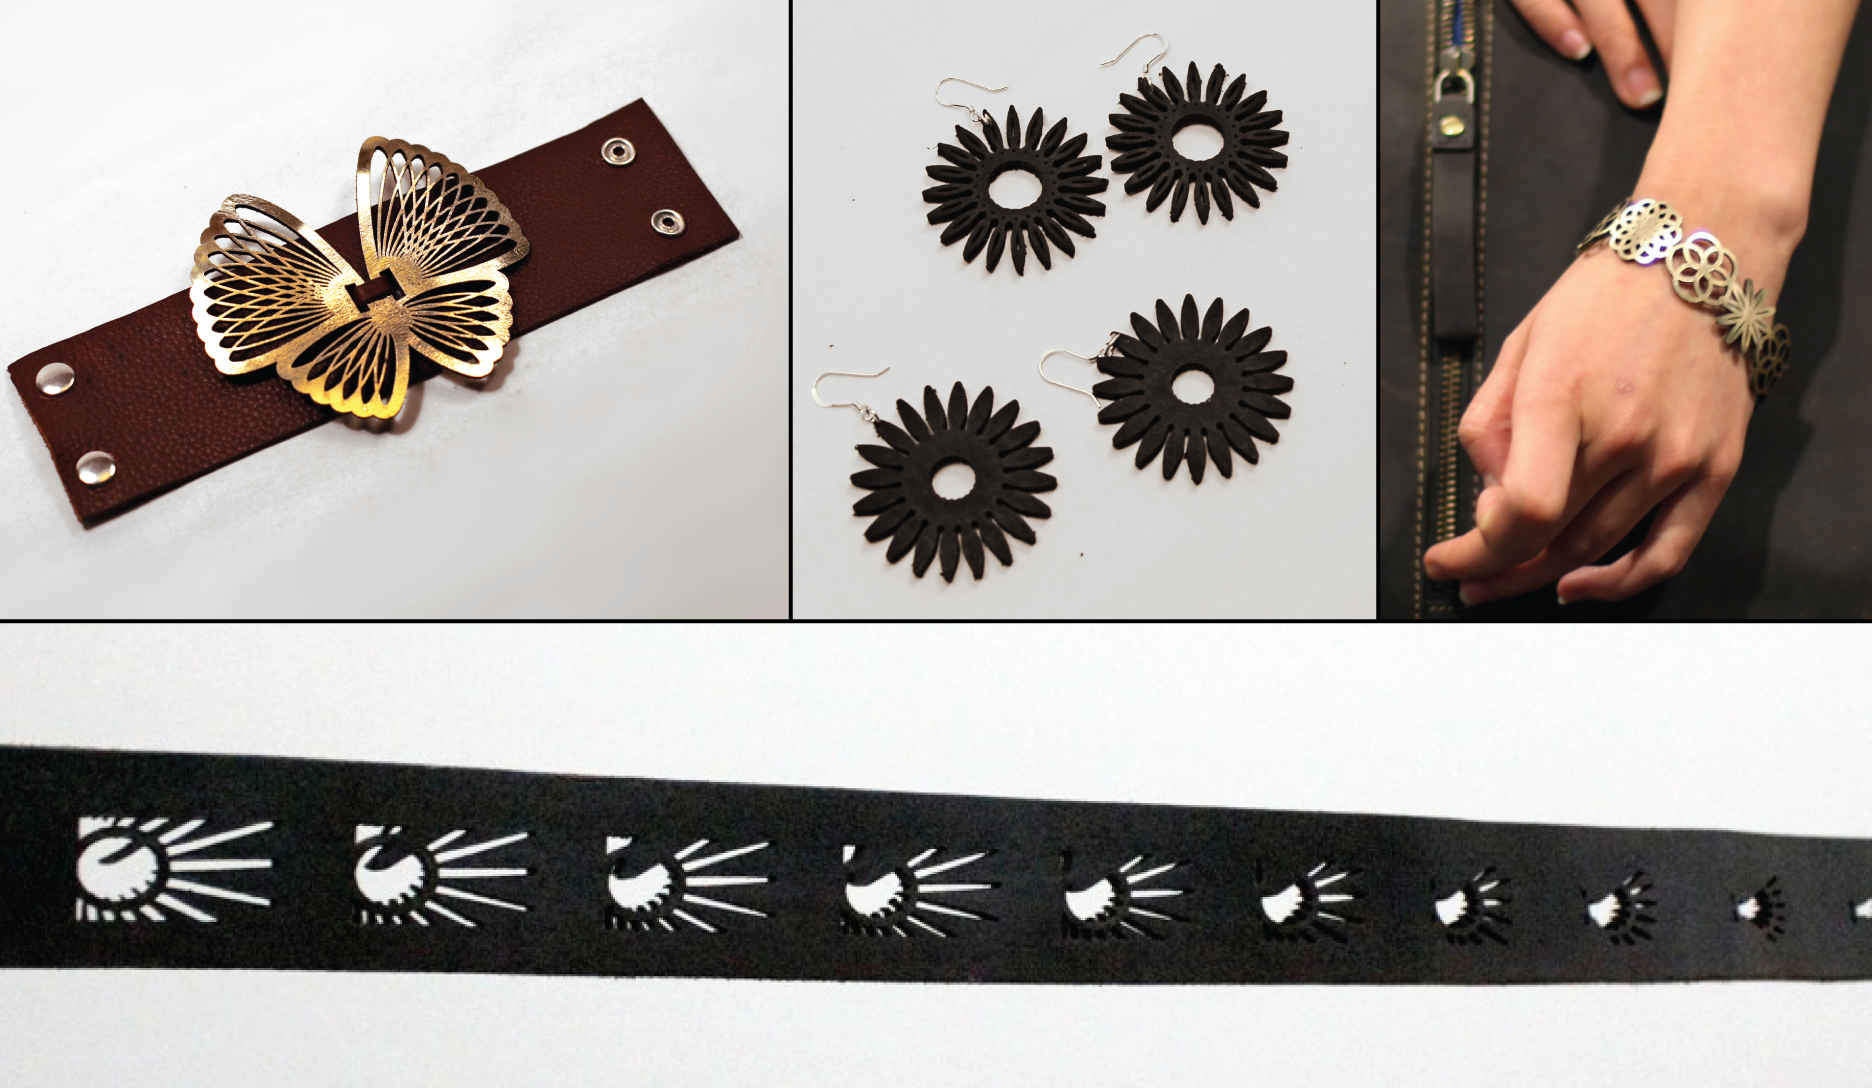
\includegraphics[width=\columnwidth]{images/expert_results.png}
\caption{a sample of the completed projects from the expert workshop (clockwise from top left: butterfly cuff, leather earrings, patent leather bracelet, algorithmic progression belt)}
\label{fig:expert_results}
\end{figure}
\end{center}

\subsection{Youth Results}
The youth workshop was more structured than the expert workshop, and produced a more consistent set of physical products as a result. All participants in the youth workshop were successfully able to use DressCode to produce a unique leather cuff (figure: \ref{fig:youth_results}.) Despite the consistency in form, the patterns and approaches among the resulting bracelets were highly varied. Each participant was also able to successfully write their own radial symmetry algorithm in the initial lesson and produce a variety of patterns with it. During the bracelet design portion, several participants directly modified the algorithm in the template to better fit their design goals, however all participants primarily relied on radial symmetry in their bracelet design. Eight of the participants  said they planned to wear the bracelets they created during the workshop, however two indicated that they planned to give them as gifts, rather than keep them for themselves. A comparison of the pre-and post-workshop surveys showed that several of the participants' comfort in programing increased following the activity. In addition, more participants indicated that they thought programing was a good tool for personal expression, and design respectively and all participants stated that they believed they could use programing to make things that were beautiful, whereas several had disagreed with this statement before the workshop.

\begin{center}
\begin{figure}[h!]
\includegraphics[width=\columnwidth]{images/youth_results.png}
\caption{a sample of the completed leather cuffs from the youth workshop}
\label{fig:youth_results}
\end{figure}
\end{center}
\section{Curriculum description}
\section{Preliminary curriculum results}
\section{Discussion}

\subsection{Enjoyment in Programing}
One of the most important points of evaluation for DressCode was how successful novice programers felt in their attempts to use it. In the Soft Objects workshop, participants were excited about the potential of programing, but unanimous in their frustration in using traditional programing syntax with the Soft Objects library, and requiring instructor assistance to execute simple actions. It is difficult to evaluate the DressCode workshop parallel to Soft Objects because the DressCode workshop took place over a shorter time period in the context of a more constrained activity. When evaluated as an independent case of novice programing however, the response in the DressCode environment by novice programmers was promising. In general the youth participants expressed  a sense of enjoyment and low levels of frustration with the coding portion. When asked if they found the programing enjoyable, participants responded in the following ways: 

\begin{quotation}

\textit{``It wasn't as hard as i thought"}
\\Youth Participant 1271996 (survey)

\textit{``[It was enjoyable] because it was very straightforward to use and easy to understand."}
\\Youth Participant 091897x (survey)

\textit{``Yes, I didn't have much experience with programming before the workshop so it was fun to screw around and see if I could push the boundaries of what I could achieve by hand."}
\\Youth Participant 091897x (survey)

\textit{``[The] computer programing was enjoyable for me because i had wanted to do it before but never had the chance. so this workshop gave me exposure to something that i wanted to do for a while. and i totally loved it."}
\\Youth Participant 092297m (survey)

\textit{``I liked [the language], it wasn't tough, it was very simple. That barrier was removed for me so I could focus on the design."}
\\Youth Participant ST
\end{quotation}

It should be noted that the last quote was from a participant who had prior coding experience. All of the other quotes came from participants who were new to programing. Some of the participants did express difficulties, however they were often described in conjunction with enjoyment or with the the recognition that through some effort, they could be overcome:

\begin{quotation}

\textit{``The computer programming was enjoyable for me; however; it was a bit frustrating and confusing at times."}
\\Youth Participant 123097f (survey)

\textit{``It was fairly enjoyable, if arduous and frustrating. Once I figured out how to do it it wasn't too hard."}
\\Youth Participant 100397c (survey)

\textit{``It was alright except a bit hard to learn but once you know it its pretty much simple for the rest of the time."}
\\Youth Participant 05231997 (survey)
\end{quotation}

Other youth participants also elaborated on the ways in which they felt programing had been useful in the design process. Their responses  evoked some of the key affordances of computational design discussed in section \ref{sec:computational_design}. For example, one participant described the advantages of programing for creating precise design elements:
\begin{quotation}
 \textit{``Basically with programing, it like- say I wanted to draw it by hand with the mouse- it would be a lot harder to make the image um , perfect's not the word..everything was scaled perfectly. Say you wanted certain shapes to be certain angles or certain sizes, if you were to code it, you can get it at the right angle, where if you were to draw it by hand, you wouldn't know what angle it is."}
 Inteviewer:\textit{`` So the precision?"}
Youth Participant N: \textit{``Yes."}
\end{quotation}

The recognition of the ability to create complex designs through repeated simple actions was another common sentiment. Again from the interviews:
\begin{quotation}
\textit{``[My design] feels complicated and simple to me at the same time- it may seem simple to me because I know the rules behind it."}
\\Youth Participant R.
\end{quotation}

Participants also discussed the parametric qualities of designing with code:

\begin{quotation}
\textit{``[I liked] the programming part.. learning different strips of code and what they did, and just changing the basic codes they gave us so basically it looks more unique"}
\\Youth Participant N

\textit{`Something that was useful about using programming to design this bracelet was that it was easy to change the sizes of the shapes very quickly."}
\\Youth Participant 123097f(survey)
\end{quotation}

Responses like these suggest that DressCode was successful in introducing participants to some of the qualities of computational design, similar to the SoftObjects workshop. Perhaps the greater success was that participants were able to implement these qualities in a more independent manner than with Soft Objects, allowing for a greater sense of personal agency, and a broad appreciation of the power of computational design. This appreciation was indicated in part by the enthusiasm of the participants following the activity:

\begin{quotation}
\textit{``Now i know that you can use computers and programing and stuff to design pretty and physically appealing things, instead of just complex robots and stuff."}
\\Youth Participant 092297m (survey)
\end{quotation}

\begin{quotation}
\textit{``It was really fun and I gained a lot of knowledge from it- knowing how to program, knowing different types of ways to manipulate shapes and radials."}
\\Youth Participant S
\end{quotation}

\begin{quotation}
\textit{``[The bracelet]  is a physical manifestation of my success in coding, maths, and programatic design, and that's what I see when I look at it. It is a little coding confidence totem that can inspire me to continue developing my skills and passion in this area - wow, I didn't realise I felt that strongly about it!"}
\\Expert Participant 090585p (survey)
%(A participant speaking about making a design for  t-shirt with DressCode) \textit{``... it's not necessarily just making a shirt with the program, but when you combine this with the %program you get the shirt, so there's endless possibilities.''}
%\\Youth Participant R
\end{quotation}

These positive reflections on the potential of programing, combined with the appreciation of specific computational affordances in design, and feelings of accessibility and feasibility of the programming process, are encouraging for a day-long programing activity with first-time coders. An analysis of these successful results in the context of  the prior workshops with Soft Objects and Codeable Objects point to several distinguishing factors. The first is related to the feature-set of DressCode itself. Although the tool still shows significant room for improvement, it appears that the simplified programing syntax, improved drawing API, and more-immediate visual feedback accounted for some of the success of the activity. By providing the participants with a small set of useful programming methods that could be used to generate complex forms and patterns, textual-computational design became relatively feasible for novices. In addition, the features in DressCode that made the transition from design to fabrication less convoluted (by not requiring any post-processing), reduced the technical concerns of the participants and allowing them to focus on using programming to design, rather having to ensure their patterns would work in a practical sense.

Another key factor in the success of the activity was the structure of the workshop itself. By relying on radial symmetry as a design mechanism, participants were given a task that had a wide range of design possibilities, but only required them to understand a few key concepts. This differed significantly from using the Voronoi diagram in Codeable Objects- an algorithm that is easy to explain in concept, but extremely difficult to implement. It also differed from the approach of the SoftObjects workshop, where the wide variety of computational approaches made it difficult to simultaneously ensure that participants designs were successful and that people understood the algorithms behind them. When a longer-term workshop is conducted with DressCode, I will attempt to expand upon the constraints of the first workshop by selecting an additional set of algorithmic patterns similar to radial symmetry in simplicity and design feasibility. Patterns such as Spirals, waves and basic fractals offer some possibilities, but there are many others.

One final element in the success of the DressCode activity was the presence of several well-prepared facilitators. For the workshop, I had four facilitators, including myself. The three additional facilitators had prior experience working with DressCode and were included in the development of the activity itself \footnote{It should be mentioned that I did have several wonderful facilitators for the Soft Objects workshop. Their presence was more sporadic however, and their involvement was not as deliberately planned as in the case of the DressCode activity.}. While a part of the facilitator assistance came in the form of addressing bugs and answering syntax questions, they were also invaluable in providing support in the design process. The other facilitators assisted participants by suggesting new design directions, helping them to evaluate their designs, and being supportive and encouraging throughout the day. Although it is desirable to strive for developing novice programing environments that allow for independent use, the benefit of well-structured in-person support should not be overlooked. Especially in the context engaging people first-time programing experiences with computational design, it is beneficial to have support staff who can simultaneously provide both technical and critical assistance. 

\subsection{Design Processes of Youth and Expert practitioners}
Because DressCode was developed to support personal visual expression through programing, a significant part of my evaluation focused on the design strategies that emerged through the use of the tool. The interviews and post surveys indicated that participants in both the expert and youth workshop engaged in a variety of design strategies in working with DressCode. When asked about her design, one young woman described a process of conscious planning. For example:

\begin{quotation}
\textit{``Well I wanted this one (pointing to an element of her bracelet) the first one made out of radial ellipses; I wanted it to look like a flower when they layer down, and the second one is kind of like the same thing, but I wanted to have the pentagon or hexagon, and the next one is the snowflake, and I wanted it to look like a snowflake because my favorite season is winter, the next one the center looks like a different sort of snowflake because all snow flakes are different, so I chose different shapes, and the last one is a rectangle-like a square in the middle and then it's like hexagons."}
\\Youth Participant S
\end{quotation}

She also described the activity as requiring ``creativity and thought and dedication", due to the high degree of complexity. When asked how she found programing useful in her design she said:

 \begin{quotation}
\textit{``You type it in and it brings it to life for you. You can do it on your own....you don't have to buy it. It's different than the casual way that somebody gets a bracelet."}
 \end{quotation}
 
Other participants also expressed conscious decisions in their design process, but also indicated that impromptu choices also played a role in their final design:

\begin{quotation}
\textit{``A few days before the workshop, I was thinking about how I will not likely wear a leather bracelet, but a belt I would definitely wear. I didn't really have an idea for what kind of algorithmic design I wanted to make. During the discussion at the beginning of the workshop, somebody used the word "evolution," and I started thinking about making a design that repeats and gradually changes across the belt. I had a hard time coming up with an interesting shape with an interesting transformation. I started with a blossom of rectangles, and tried a bunch of variations. At some point somebody said it was like an animation, which gave me some positive energy in thinking about the design (and I thought I could be a human zoetrope, spinning in sync with a strobe). It started to get more interesting when I added the masking effect. I eventually made the individual pieces making up the ellipses instead of rectangles, which both made the thing softer, and emphasized the transition as they collide with the mask, forming sharp corners."}
\\Expert Participant 071279R (survey)
\end{quotation}

\begin{quotation}
\textit{``I saw that the duplication of a large shape was kind of happening with a lot of people's designs, so I decided to try and do something a little different. (Show's a first design (ellipses side by side on a line). That was the second phase of this, and then I just started screwing with numbers to see what I could get and I came up with this. I didn't know if I wanted the entire thing to be symmetrical or not, but then I thought that that was getting too boring (the symmetry), so then I changed the number of shapes in the loop to an odd number instead of an even one so that it would offset the design, and came up with this."}
\\Youth Participant R
\end{quotation}

\begin{quotation}
\textit{`I kind of like started off playing around with the main stuff and once I got that I narrowed it down and tried to switch around different parts to see which parts worked best."}
\\Youth Participant C
\end{quotation}

\begin{quotation}
\textit{`I used an example I liked and decided to spend time doing an earring or single pendant so I could focus on manipulating the example to see how the program worked. I also picked something that repeated the same unit for simplicity and the time limit."}
\\Expert Participant 081764
\end{quotation}

Youth and expert participants varied in the levels of intention in the design process. Because of their professional experience and education, on average the expert participants approached the activity with a greater level of deliberation and were better able to articulate their design process. However, the responses from the youth practitioners demonstrate that they also felt they were able to make conscious design decisions in a programing context. Deliberate design choices were also made based on the materials available. Participants made decisions based on the material properties of the leather as it folded or bent, and considered the fact they were planning wear the resulting piece:

\begin{quotation}
\textit{``The ellipse [in the design] was added once I understood that the teeth sticking inward in the design (formed by the inverse of the ellipses sticking outward) would pop out from the surface of the belt when it was curved around my waist- I saw this when we made a paper prototype. The ellipse held the teeth in place."}
\\Expert Participant 071279R (survey)
\end{quotation}

\begin{quotation}
\textit{``I deliberately made it more delicate and feminine, because I'm putting it on black leather, I just made it a lot prettier- with thinner lines- I have more thin than thick."}
\\Youth Participant J
\end{quotation}

\begin{quotation}
\textit{``Well, I printed out the different widths of the line because if you're going to wear it, you want it to be durable. The thinness of it, I don't want it to be easily ripped, rather than if I was like a thing to hang on a wall, I could just do anything I wanted, because it's not like it's going to have to withstand any elements. And you want it to look nice because I care about what I wear, cause what you wear, you're presenting an image of yourself to people."}
\\Youth Participant R
\end{quotation}

A few adult and youth participants  relied on an experimental design approaches, or came to their final design through trial and error:

\begin{quotation}
\textit{``You just have to fool around with it until you like how it comes out."}
\\Youth Participant G
\end{quotation}

\begin{quotation}
Youth Participant S: \textit{`I just typed it in and started messing around with this, and then I gave it a go."}
\\Interviewer: \textit{``How did you know you were done with it?"}
\\Youth Participant S:\textit{`` I ran out of ideas."} 
\end{quotation}

\begin{quotation}
\textit{``[I decided on the design] mostly through trial and error, I found what was easy/reliable to do but looked interesting. I spent some time rounding out the form of the bracelet, this was the most directed portion of the design process."}
\\Expert Participant 081764
\end{quotation}

Experimentation through trial and error can be a useful tactic, however too much reliance on this form of design can result in a diminished sense of accomplishment. As one participant stated, he enjoyed the design process at first, but for him:

	 \begin{quotation}
	  \textit{``the more "trial and error" kind of ruined it a little. The more anyone messes up with anything it kind of takes away the fun from it of it. But then the end result made up for it. "} \\Youth Participant N
	 \end{quotation}

Control over one's design plays a large part in the experience of the designer. Whether their choices were made through forethought, or realized mid-process, that ability of participants to realize their design objectives through programming had a positive impact on their experience. The participants who articulated intention in their design process emerged with a greater feeling of ownership over the finished artifact, and a more positive view of computational design than those who felt they relied on trial and error. In the case of computational design with novice programmers, conscious design processes can be difficult to achieve. The advantage of DressCode over SoftObjects and Codeable Objects was that it enabled designers to make changes and quickly see the results of these choices in their design, allowing for  a greater level of control. In the case of participants who felt they relied on trial and error, future tools should endeavor not only to make  computational design more accessible, but also assist in the communicating the history of a design to a designer.  This may provide them with better sense of their process, and give them better platform upon which to base future decisions.  

\subsection{Computational Aesthetics}
\begin{comment}
\begin{quotation}
\textit{``Instead of doing something that I thought would look cool, I tried to think of something I would generally wear, I didn�t pick bright pink, because I knew I would never wear that."}
\\Youth Participant K
\end{quotation}

\begin{quotation}
\textit{``I have multiple designs that I'm just kind of playing around with. But I think I'm going to do this one, and by this one I mean one variation of these (style), because the only thing that changes is the width of the actual lines. So this kind of doily lace one, I guess. Yeah, it reminds me of a lace doily or something, and this would kind of offset it (referring to the leather)"}
\\Youth Participant R
\end{quotation}

Sense of uniqueness
\begin{quotation}
\textit{``I think it's interesting. I'm assuming this design is unique to me unless someone else goes and makes exactly the same thing, which I highly doubt because of all the random calibration things that I ended up adding."}
\\Youth Participant C
\end{quotation}
beauty
\begin{quotation}
Interviewer: \textit{``Do you think your design is beautiful?"}
\\Youth Participant R: \textit{``No� if it is, it's because of the program, not because something unique I brought to it.. ok I think they're all kind of beautiful- ok I just completely changed my answer. It reminds me of stained glass and I think stained glass is really beautiful."}




\textit{``I tried to contrast ellipses shapes with the more geometric looking ones."}
\\Youth Participant C
\end{quotation}


Personally relevant aesthetics through computation
\begin{quotation}
\textit{``usually when you make something you're making it like �oh I hope society likes this� but this[making the bracelet] was about self satisfaction, so I don't have to take into consideration someone else's opinion."}
\\Youth Participant S
\end{quotation}

emergence of narrative aspects
\begin{quotation}
\textit{``The rose right there, and then the scientific part of it, those two things I like- nature and science, but sometimes nature conflicts with science. I want to do aerospace engineering when I get to college, but aerospace engineering conflicts with the environment in some ways, aerospace has to do with machines so that means a lot of gas is burning stuff like that. "}
\\Youth Participant S.M.
\end{quotation}

social qualities of crafting - maybe for a future direction
role of critique in the process - maybe for a future direction

\end{comment}

\subsection{Starting notions of craft and computation}
When developing a tool for combining craft and computation, it is important to understand people's prior conceptions of these domains. In the case of the DressCode study, there was a strong distinction between the views of the two groups of participants on the respective roles of craft and computer science. During the expert discussion, two separate forms of craft were discussed. The first referred to craft as hobby and amateur practice. The experts also demonstrated an appreciation for craft as an artisinal practice, wherein handcrafted artifacts held higher value than mass produced ones because of the time and expertise required for their production. In the youth discussion of craft, the recognition of craft as artisanal practice was completely absent. Instead they referred to craft as an recreational activity, that anyone could do. The perception of craft as open and accessible by young people is encouraging, however many youth participants also dismissed the difficulty of craft in comparison to programing. One young woman articulated her view on the difference between writing a program and throwing pottery, stating that she knew she could throw a pot, but that she would be unable to write a program, despite having no prior experience in either medium.  The variation in expert and youth perspectives on the levels of expertise present in craft is understandable, given the educational differences between the two groups. 

There was also a difference between the amount of variation in the crafting processes between the two experts and young people. Several participants in the expert group experimented with layering different materials on top of one another for a different effect. One participant sewed a portion of her project rather than attach portions with snaps. Another used the snaps as an aesthetic component, by placing them across the length of the piece and then snapping on different colored pieces of leather in different patterns. There was limited variation in the approaches the youth practitioners took in the crafting portion. Furthermore, many of the youth participants remarked on the surprising difficulty of the handcrafting component.

\begin{quotation}
\textit{``Something that was difficult was hammering the snaps in straight enough for them to function well."}
\\Youth Participant F

\textit{``It was enjoyable being able to wear it and making sure that it would fit. It was a little stressful figuring out how to put the clasp on. "}
\\Youth Participant K

\textit{``I think the actual physical copy [of my bracelet] is slightly less attractive than the one I had on the computer."}
\\Youth Participant C

\textit{``I hate being anxious because I don't know if it's going to come out right. I like the designing on the computer, but once it comes out it looks like crap. So I'm really happy that I came to this (workshop), this is the first one that came out."}
\\Youth Participant ST

\end{quotation}
\begin{comment}
continued excitement w/ laser cutter
\begin{quotation}
\textit{``I was excited- I was really happy when it came out. Even though I've used laser cutters, the ones at our centers aren't powerful enough to do something like this.
This is probably the most complex thing that I've done with a laser cutter."}
\\Youth Participant ST
\end{quotation}
\end{comment}
It is likely that there is a connection between people's perception of craft, and their ability to engage in new crafting techniques, despite encountering difficulties along the way.
\todo{section currently not complete}
\begin{comment}
\begin{quotation}
\textit{``It's just a whole new program, it's not something that I already know how to do. Arts and crafts is like, anybody can do it, but here you need to follow what [the instructor] says, you need to know what you're doing ... I think you just need to have more fore-hand knowledge to know what to do."}
\\Youth Participant S.M.
\end{quotation}


interest in longer design time, appreciation of needing to learn more
\begin{quotation}
\textit{``Often when I'm doing art and I take a break from it and come back to fresh eyes, then I'll realize that I can do something differently or get something better"}
\\Youth Participant S.M.
\end{quotation}

\begin{quotation}
\textit{``I would love to get into more computational design, I think it's really really cool, because I'm an amateur graphic designer as well. I'm a self-taught programmer, so I want to get into  that [computational design] because it's really cool."}
\\Youth Participant ST
\end{quotation}
\end{comment}
\subsection{Relation to Other Design Tools}
\begin{comment}
importance of not starting with blank page

\begin{quotation}
\textit{``I'd rather just have something set and she would just show us how to manipulate the stuff here and it would be easier, instead of showing us all the functions you could do. I would rather have something set for you you, and all I have to do is just plug in numbers."}
\\Youth Participant S.M.
\end{quotation}

\begin{quotation}
\textit{``I've never really done programming like this, but once you have the whole format in and you're just down to changing the numbers then it's fine, but before that if you're not typing something in correctly and you can't find what it is.. but this is relatively simple."}
\\Youth Participant R
\end{quotation}

\begin{quotation}
Interviewer:  \textit{``Would you want to use DressCode again?"}
\\Youth Participant R:\textit{``Sure yeah, now that I feel more comfortable with it and could just start doing it, rather than having to learn. I think it's a good program for someone who's never done anything before...}

\textit{....There's a t-shirt and the symbol on it you can tell was made in here and just attached to the shirt it's not necessarily just making a shirt with the program, but when you combine this with the program you get the shirt, so there's endless possibilities.''}

\end{quotation}


interest in continuing  but comfort in traditional tools
\begin{quotation}
\textit{``I'm more of a sketchup person. I need it directly. I can't program and then play it and then it goes."}
\\Youth Participant S.M.
\end{quotation}

\begin{quotation}
\textit{``They all require some kind of digital design program. We just used DressCode, but what I use is Inkscape or libre office to design my stuff, so it's kind of the same process."}
\\Youth Participant N
\end{quotation}

\begin{quotation}
\textit{``I don't know if this is my preferred medium, but I definitely like it.  Making other accessories. If I spent more time playing around with it, I could definitely get something good. 
I'm glad I did it, it's interesting, It's something that I don't have a lot of experience in- just branching out."}
\\Youth Participant R
\end{quotation}
\end{comment}

\subsection{Pride and Accomplishment in Algorithmic Craft}
\begin{comment}
\begin{quotation}
Youth Participant J: \textit{``It's on computers and I'm terrible at computers and for me to actually get something like this is really big."} 
\\Interviewer:  \textit{``How do you feel about that?"}
\\Youth Participant J:  \textit{``Really proud."}
\end{quotation}

\begin{quotation}
 \textit{``II think [the programming] kind of reminded me of learning something difficult in like math, because I don't really like math, but when I figure out something, then I start doing it, and can do it and then I feel proud of myself"}
 \\Youth Participant C
\end{quotation}

\begin{quotation}
 \textit{``I thought it was a good experience, It was different and it sort of opens your mind to thinking about what else you could do with programing, fashion and stuff like that."}
 \\Youth Participant J
 \end{quotation} 
 
 \begin{quotation}
 Interviewer:  \textit{``What stands out to you about your design?"}
 \\Youth Participant S.M.: \textit{``That I actually created it. I'm not really a programing person, doing it and typing it out."}
 \end{quotation}
 
 feminine and masculine aesthetics
\begin{quotation}
 \textit{``I think it is beautiful for females. Not me. Because, I don't go that way. Because on a female's wrist it looks right� not on mine."}
 \\Youth Participant G
\end{quotation}

Joking- but serious implications behind humor
\begin{quotation}
 \textit{``Wow that's manly. Then I put it on my wrist and I was like wow that's feminine. That's very feminine."} \\Youth Participant G
\end{quotation}
\end{comment}

\subsection{Design history and selection}
\begin{comment}
\begin{quotation}
\textit{``As you can see saved 10 different versions so I would save something, not a completed version of it, but as I was going a long and just do random things to it and see what happened, and if I was physically drawing it, I couldn't just do that unless I wanted to just keep erasing and re-drawing, but in this it's simple as just typing in another number and it will change, but you can always go back to what you had, so it's nice like that."}
\\Youth Participant R
\end{quotation}
\end{comment}

\subsection{Prototyping pt 2}
\subsection{Connection to other applications}
\subsection{ challenges in crafting}


\chapter{Conclusion and Future Directions}
	
	I began this thesis with a creative interest in computational design and digital fabrication, and a personal history of making things by hand. My assumption was that a synthesis of these practices might appeal to other people, especially those who were new to programing. Following my experiences in developing  tools and conducting workshops, it is clear that  algorithmic craft resonates with many people, from young people, to experienced programmers, to artists and designers. Furthermore, algorithmic craft promotes the values of personal relevance, craftsmanship, beauty, intellectual engagement and pleasure in making. I conclude this thesis with a set of guidelines for future algorithmic craft tools and practices:
	
		\begin{itemize}
		
		\item \textbf{Tools should support design techniques that demonstrate the benefits of computational design.}  Algorithmic crafting tools should effectively communicate the affordances of computational design in ways that are accessible to new programmers. This can be achieved by providing programing examples which suggest design approaches or by creating built in programing methods with compelling aesthetic potential.  The radial symmetry algorithms in the DressCode study provide one example. By relying on radial symmetry as a design mechanism, participants were given  a wide range of design possibilities, in a format that was relatively easy to understand. Algorithms that produce spirals, waves and basic fractals offer some possibilities for introducing new programmers to computational design. 
				
\item \textbf{The software interface should prioritize interaction through programing.} Programing should be the chief method of generating and manipulating designs, and this focus should be reflected in the interface of the software. The visual design that is produced by the program should be persistent in the software interface and be rapidly updated to reflect changes in the user's code. It is also helpful to provide additional visual feedback through simulation of a finished artifact- as in the case of the 3D preview in Codeable Objects. It should be noted that this form of simulation presents a significant technical challenge for more complex artifacts.

\item \textbf{Programing languages should have a design-oriented programing syntax, developed with novice programmers in mind.} The programing syntax and API should be designed to accommodate individuals with no prior programing experience, and should be limited to methods and structures relevant to the task of design. By providing users with a small set of useful programming methods that can be used to generate complex forms and patterns, it becomes feasible for novices to engage in intentional and independent computational design.

\item \textbf {Tools should reduce the technical challenges of digital fabrication.} The software should include programing and drawing methods that allow for the production of designs that are suitable for digital fabrication and support for exporting to relevant file formats. The transition from the design tool to the fabrication device should require as few intermediary steps as possible. When possible, it is useful to add in methods that help people ensure their design will fabricate as desired. This may include merging all polygons of the same color into one complete path, or automatically optimizing lines to increase fabrication speed. 

\item \textbf{ Software tools should be free and open-source.} The software should be freely available, and able to function on multiple platforms with low requirements for computational processing power to afford high levels of access to casual users. If possible, the software should also be open source, in order to encourage the proliferation of additional novice oriented tools that can be developed for the specific needs of distinct user groups. 

\item \textbf{Activities should blend domain specificity with creative openness.} To encourage the creation of personally relevant aesthetics algorithmic craft tools should be open enough to support numerous creative applications. This openness should be tempered by introducing the tools in a way that provides users with a compelling motivation for their use. For first time users, algorithmic craft activities should be constrained to the design of a limited set of end products, with the potential for aesthetic variation. In more general design scenarios, It may be useful to engage designers by asking them to create artifacts which express a specific feeling or emotion, represent a character, or tell a story. Design briefs such as these may further people's conception of how computational design can be used to create personally relevant artifacts, and result in an even broader set of aesthetic possibilities.

\item \textbf{Tools should be supported through fabrication and craft-specific documentation.} In addition to the documentation of the application and programing language, the fabrication and crafting techniques intended for use with the software should be well-documented. This documentation should include details on suitable materials, fabrication machine access and settings, and tutorials on the craft components of example projects.

\item \textbf{Activities should encourage discussion and group critiques of work, and when possible, use in-person facilitation and guidance.} Algorithmic Craft is a creative practice, not a technical exercise. Algorithmic craft activities benefit from discussion among peers, critique and reflection. With novice programmers, this form of engagement is best conducted in a group setting with some form of facilitation. Facilitators can provide assistance in addressing bugs and answering syntax questions, while simultaneously encouraging people in thinking about their designs. 

\item \textbf{Materials Matter.} The use of rich and interesting physical materials greatly enriches the experience of algorithmic craft, and contributes to the success of the finished artifacts. Raw materials like leather, wood, textiles and art-quality paper provide a compelling contrast to the precision and complexity of computational design and digital fabrication, and can produce objects that are not only attractive, but durable. Care should also be taken to use construction techniques that will hold up over time. Use archival adhesives, and be especially thorough in the construction of artifacts that are meant to be worn.\footnote{Also, if you purchase a large amount of leather, don't leave it near the recycling bin overnight.}
\end{itemize}


\section{Future Directions}

	There is considerable future research to be done in algorithmic craft. The software tools that support algorithmic craft provide continued opportunity for innovation.  By improving the ways in which a tool communicates the functionality of a program, it is possible to improve the experience of the designer and the range of what they can accomplish when using the tool. At the moment, I am adding a declarative design view into the DressCode interface (figure:\ref{fig:declarative_view}) that displays a listing of all of the components in the design, and shows their relationships to one-another. Such a feature could enable a person to manipulate their designs in an imperative form through the programing interface, or by directly altering the properties of individual primitives in the declarative view, depending on what was most appropriate for their current design objective.

 \begin{center}
\begin{figure}[h!]
\includegraphics[width=\columnwidth]{images/declarative_view.png}
\caption{DressCode with declarative view of a design}
\label{fig:declarative_view}
\end{figure}
\end{center}

Another important area of future research is in maintaining design history and assisting in design selection. A common challenge encountered by many participants in the DressCode workshops, was the process of choosing a single design for fabrication, out of numerous possibilities: 

\begin{quotation}
\textit{``As you can see saved 10 different versions so I would save something, not a completed version of it, but as I was going a long and just do random things to it and see what happened, and if I was physically drawing it, I couldn't just do that unless I wanted to just keep erasing and re-drawing, but in this it's simple as just typing in another number and it will change, but you can always go back to what you had, so it's nice like that."}
\\Youth Participant R
\end{quotation}

As mentioned earlier, the issue of design selection is not unique to DressCode, but an inherent quality of computational design. Because algorithmic craft depends on the creation of discrete physical artifacts, design selection in algorithmic craft is a more urgent issue than in other forms of computational design. Future research could explore methods of evaluating numerous designs and in providing people with mechanisms for selection. 

Related to the issue of design selection is that of design history. Participants in all of the workshops often created designs that were later lost due to numerous changes in their code. They also often wished to merge components of two separate designs, or selectively undo some but not all of the changes to a new design. All of these challenges suggest the need for some form of version control in algorithmic craft software. If implemented correctly, version control could not only give people better control of the history of their designs, but also increase the ability to share work, and contribute to the work of others.

Finally, more research must be done in incorporating the practices and values of craft. Although craft was one of the founding components of this thesis, much of the development time was focused on writing software and learning about the properties of digital fabrication. For future research, I wish to seek the expertise of established craftspeople to gain a better understanding of craft practices and how they can be connected to computational design and digital fabrication. One possibility would be to engage in the collaborative design of a sample algorithmic crafting tool with a group of people who are experienced in a particular form of hand-craft, like garment creation or jewelry making.

\section{Conclusion}
	As computers grow in sophistication, complexity and ubiquity, it becomes possible to regard computation as a dismebodied force, outside the reach of most individuals, and incompatible with familiar forms of making. In my experience, the opposite is true. Computers offer one of the most potent forms of personal expression, by helping us to see the world in new ways. Computation does not invalidate other forms of creation, it enhances them. Algorithmic craft gives people the opportunity to experience the magic and pleasure that is possible when using programing, digital fabrication and one's hands to build something entirely new. 
	
	
	
	
	
	
	
%% This is an example first chapter.  You should put chapter/appendix that you
%% write into a separate file, and add a line \include{yourfilename} to
%% main.tex, where `yourfilename.tex' is the name of the chapter/appendix file.
%% You can process specific files by typing their names in at the 
%% \files=
%% prompt when you run the file main.tex through LaTeX.
\chapter{Future Directions}

	
	Version Control (The loss of design)
	Better selection mechanisims
	Longer-term studies
Targeted audience (revised)
Importance of in-person instructors- in relation to craft related activities

\include{chap10}
\appendix
%\chapter{Tables}

\begin{table}
\caption{Armadillos}
\label{arm:table}
\begin{center}
\begin{tabular}{||l|l||}\hline
Armadillos & are \\\hline
our	   & friends \\\hline
\end{tabular}
\end{center}
\end{table}

\clearpage
\newpage

%\chapter{Full DressCode Language Specifications}

\subsection{Interface Design}
 \begin{center}
\begin{figure}[h!]
\includegraphics[width=6.5in]{images/dress_code_interface.png}
\caption{The DressCode interface}
\label{fig:dress_code_interface}
\end{figure}
\end{center}

The interface of DressCode is divided into two sections, a design panel and a coding panel. The divider between the two panels can be resized as needed. The coding panel contains a primary window for entering text, an output console for print output and error reporting and a row of buttons on the top. When the play button is pressed, the program in the code window is run and the resulting design is displayed in the design panel. The first version of DressCode ran the code each time the enter key was pressed or a new statement was completed, however we received many requests from our initial user tests for manual control of the run process. The stop button attempts to terminate programs that are taking too long to run.The following three buttons allow for the creation of new programs and the saving and opening of existing programs. The final button opens a dialog that enables the user to select an Scalable Vector Graphics (SVG) file to import into their script (the rationale for this is described in \ref{par:shape_transformation} section below.)

The design panel is primarily composed of the drawing canvas. The drawing canvas has a set of rulers and a grid, along with a black rectangle in the center which serves as the drawing board. The drawing board defines a reference for the coordinate system of the canvas, with the upper left hand corner corresponding to (0,0) in cartesian coordinates. Designs can be drawn on any part of the canvas, including outside the drawing board, however the exported designs file-dimensions will always correspond to the size of the drawing board. The right-most button in the design panel allows for the specification of the units of the project, and the resizing of the drawing board. The print button opens a dialog that allows the user to export their current design in a vector format. I experimented with various vector file formats including DXF, SVG and PDF, however for the time being, I settled on PDFs as they were compatible with the specific fabrication machines I intended to use in my workshops. 

The grid button allows the user to toggle between a grid in the units that correspond to the current units of the project (either millimeters or inches), pixels, or no grid. The target button allows the user to graphically select a set of coordinates and have them appear in the programming window as text, and can be used like an eyedropper for pixel coordinates. The plus and minus magnifying glasses and the hand tool are used to pan and zoom in and out of the screen.  Lastly, the arrow tool allows for design elements to be graphically selected and manipulated. After a design element is moved with the arrow tool, with the corresponding code for the move appears in the programing window. 

\subsection{Programing Language}
The DressCode programing language is interpreted with semantic functionality that is simulated through a Java-based library.  We relied on the ANTLR framework to generate the necessary lexing and parsing methods for the language, and developed the semantic functionality using java and the java openGL (JOGL). When a program is run in DressCode, the raw script is first tokenized and then parsed to generate an abstract syntax tree (AST). During this phase, all user-generated function definitions are stored in memory. If any parsing errors are encountered, they are output to the console as "compiler errors". Assuming the parse is successful, DressCode then walks the resultant AST and attempts to execute the semantic functionality of the program (figure:\ref{fig:interpreter_structure}.) After being executed, the resultant design is rendered on the display panel. Any runtime errors are displayed in the output console. For most programs, this process is instantaneous, however some programs with complex operations require several seconds to be executed. 
  \begin{center}
\begin{figure}[h!]
\includegraphics[width=6.5in]{images/interpreter_structure_horz.png}
\caption{Interpreter structure}
\label{fig:interpreter_structure}
\end{figure}
\end{center}
The language is imperative in nature, with statements being executed in the order in which they are read. The exception to this is user defined functions, which may be defined at any point in the program, and called before they are defined. Each statement in DressCode must be terminated by a semicolon. I spent some time experimenting with terminating statements with newlines, similar to whitespace sensitive languages like Python, as I thought this might be more conducive to novice use. Unfortunately, the implementation of selective whitespace recognition is a challenging task to define in a grammar, so while we were able to develop a version of DressCode that recognized statements terminated by a line break, it would have taken significant time to develop this functionality to a level of robustness appropriate for user testing. For the short term, we have opted for a syntax requiring semicolons, however we plan to continue to explore newline statement termination in the future. 

\subsubsection{Language Structure}
Here, I define some of the primary elements of the DressCode syntax and drawing API, and the rationale for their structure. A more thorough language reference is available on the DressCode wiki\cite{DressCodeWiki}.

 DressCode supports number, string, boolean, and drawable datatypes (figure \ref{fig:basic_datatypes}.) The first four of these types are relatively standard in comparison to conventional programing languages. Numbers include integers and floating point values. Strings include any sequence of characters enclosed in double quotations. Booleans have two possible values: true, and false. Drawables are a special type, discussed in detail in the API description below. DressCode also contains a list data structure, which can store multiple kinds of datatypes.
\begin{center}
%\begin{figure}
\begin{lstlisting}
myString = "hello";  //string
myNum = 10.4;  //number
numbermyBool = true;  //boolean
myList = [10,11,false,"world"];  //list with multiple data types
println(myList[3]); //prints world
\end{lstlisting}
%\caption{basic datatypes}
%\label{fig:basic_datatypes}
%\end{figure}
\end{center}

Variable identifiers in DressCode must begin with a letter which followed by 0 or more letters or digits. Variables can be initialized through assignment, or declared and assigned later in the program. All assignment in DressCode is dynamically typed, and variables can be assigned to datatypes that differ from their original assignment at any point. %(figure \ref{fig:variable_assignment}.)

\begin{center}
%\begin{figure}
\begin{lstlisting}
s1 = "hello";
s2 = "world";
s3; //variable without initial assignment

s3 = s1+" "+s2; 
println(s3); //prints hello world

n1 = 2;
n2 = 2.5;
println(n1+n2*10); // returns 27.0
\end{lstlisting}
%\caption{variable assignment.}
%\label{fig:variable_assignment}
%\end{figure}
\end{center}

The  language also contains support for basic expressions, as well as block statements, including conditionals, loops and user-defined functions. For mathematical expressions, standard order of operations is maintained, unless parentheses are introduced. All block statements are signified by a keyword followed by a colon, and terminated with the end keyword which is not followed by a semicolon.Conditionals are defined with the if keyword, and may an optional else clause and  zero or more else if clauses. %(figure: \ref{fig:conditionals}.)

\begin{center}
%\begin{figure}
\begin{lstlisting}
//if statement 
if 5<10:
println("true"); //prints true
end

//if statement with else if and else clause
i=10;
if i<10:
println("less than 10");
else if i==10:
println("equals 10"); //prints equals 10
else:
println("greater than 10");
end
\end{lstlisting}
%\caption{conditional definitions}
%\label{fig:conditionals}
%\end{figure}
\end{center}

There are two possible loop statements: repeat statements and while statements. Repeat statements begin with the repeat keyword and are followed by a the initialization: a variable identifier with a numerical assignment, followed by a colon and the test, a number that determines the point at which the repeat statement will terminate. By default, all repeat statements have an update value of 1, however this can be modified by following the test value with "add" and a 3rd value specifying the update condition. While loops are initialized with the while keyword and followed by a test condition.%(figure: \ref{fig:loops}.) 

\begin{center}
%\begin{figure}
\begin{lstlisting}
//repeat statement
repeat i=0:10:
ellipse(0,i*10,10,10); //draws a vertical row of 10 ellipses
end

//repeat with modified update condition
repeat i=0:10 add 2:
println(i); //will print 0,2,4,6,8
end

//while statement
c=0;
while c < WIDTH:
ellipse(c,10,20);
c = c+20;
end
//draws a row of ellipses that span the width of the canvas
\end{lstlisting}
%\caption{loop definitions}
%\label{fig:loops}
%\end{figure}
\end{center}

Finally, custom functions are defined with the def keyword, followed by an identifier and a set of parentheses containing 0 or more arguments separated by commas. The function block is terminated with the end keyword like all other block statements. Just like general assignments, functions arguments are dynamically typed. Functions, loops and conditionals all have their own scope and will prioritize identifiers based on that, however if they cannot locate an identifier within their own scope, they will look for it in the level above.
\begin{center}
%\begin{figure}
\begin{lstlisting}
//basic function defintion
def foo(a,b,c):
println(a+b+c);
end

//function call
foo(1,2,3);  //prints 6

//function with return statement
def bar(a,b,c):
return(a*b*c);
end

result = bar(4,5,6)); 
println(result);//prints 120
\end{lstlisting}
%\caption{loop definitions}
%\label{fig:loops}
%\end{figure}
\end{center}

\subsubsection{Drawing API}
 The API is organized around the creation and transformation of 2D shape primitives. By duplicating and manipulating these primitives in a structured manner, it is possible to generate complex and interesting designs from simple forms. The API is composed of three primary main categories, divided by functionality: shape primitives, shape transforms, shape booleans, math operations and property access. A selection of the primary methods from each of these categories is detailed in figure \ref{fig:api_table}. 

  \begin{center}
\begin{figure}[h!]
\includegraphics[width=6.5in]{images/api_table.png}
\caption{A selection of methods from the DressCode API}
\label{fig:api_table}
\end{figure}
\end{center}
\paragraph{Shape Primitives:}
DressCode shape primitives currently serve as the primary means of drawing (figure: \ref{fig:shape_primitives}.) The simplest primitive is a point, initialized two numerical parameters that denote the x and y coordinates. All closed-shape primitive methods (ellipses, rectangles and polygons) require an argument of either two x,y coordinates, or a point. This coordinate defines the origin of the shape and determines where  the shape will be drawn on the canvas. Ellipses and rectangles have an additional two optional parameters which specify width and height. If only two arguments are provided, the ellipse or rectangle will be drawn with a default width and height; if three arguments are given, the width and height will be the same. Polygons also have two optional parameters following the x and y origin coordinates, however they specify number of sides and length of each side, rather than width and height. Lines can be initialized either as four numerical values, specifying start and end x and y coordinates, two points, or as a vector, with a origin point,  a magnitude, and a heading in degrees. Curves are defined by a set of four points or eight coordinates, which determine the start, first control point, second control point and end point of a 4-point bezier curve. One other method of primitive generation was added in at the request of some of our early users: vector paths stored in Scalable Vector Graphics (SVG) format can be imported and drawn in the DressCode environment, and used in conjunction with primitive transformation and boolean methods.  

 \begin{center}
\begin{figure}[h!]
\includegraphics[width=6.5in]{images/primitives.png}
\caption{DressCode shape primitives with visible origins}
\label{fig:shape_primitives}
\end{figure}
\end{center} 

\paragraph{Shape Transformations:} \label{par:shape_transformation}
There is no required "draw" method for DressCode, as there are in many other graphics APIs, Instead all primitives are automatically drawn in the display panel in the order of their initialization, once the program has been run. In Soft Objects and Codeable Objects, when we required users to manually call draw method for any and all shapes in their program, they often forgot, and then had difficulty determining the reason why parts of their designs were not visible. 

Each shape primitive method returns an instance of the primitive it creates. A programmer can either create shapes with no reference as in figure \ref{fig:shape_primitives}, or they can assign them to an identifier at initialization, allowing them to reference and modify the shape later in the program. The shape transformation methods allow for a range of modifications to a shape, by passing a reference to the primitive the first argument, followed by different parameters for the modification, depending on the method (figure: \ref{fig:transformation}.) We began with a basic set of transformations, including move, rotate, methods that allowed for the modification of the stroke weight and color of the shape, and a hide method that prevented a primitive from being drawn. Based on our early user testing however, we gradually added in additional methods, based on what people wanted to do with their designs. This included a moveBy method, scale and mirroring functionality, a copy method, and an addition to the rotate method which allowed a shape to be rotated around a point other than its origin. 

 \begin{center}
\begin{figure}[h!]
\includegraphics[width=6.5in]{images/transformation.png}
\caption{SVG import and sample of transformation methods}
\label{fig:transformation}
\end{figure}
\end{center} 

DressCode primitives can also be programmatically "grouped". Grouping provides an organizational structure for more complex configurations of primitives allows for the automatic transformations to multiple shapes. Groups have their own origin, which is used as the reference point for all move, rotation and scale methods applied to the group (figure: \ref{fig:grouping}.) For example, a collection of ellipses that is grouped and then moved to the center of the canvas would move the origin of the group to the center, and all the ellipses relative to the new origin. The origin of a group is automatically calculated as the centroid of all of the objects in the group and updated each time a primitive is added or removed. Groups are treated similarly to lists in that individual objects can be accessed and manipulated by via their index. Originally, primitives within a group were transformed relative to the origin of the group, however this caused confusion among many of our initial users. Each individual primitive is now translated according to the coordinate system of the canvas, regardless of whether it is in a group. 

 \begin{center}
\begin{figure}[h!]
\includegraphics[width=6.5in]{images/grouping.png}
\caption{Grouping with transformation and repeat statements}
\label{fig:grouping}
\end{figure}
\end{center} 

\paragraph{Polygon Booleans:}
DressCode also features a subset of transformation methods for polygon boolean operations (figure: \ref{fig:boolean}.) The union, difference, exclusive or and intersection methods accept two primitives as arguments and return the corresponding shape, or group of shapes, depending on the operation. In addition, the merge method performs a union on all objects within a group and returns a single primitive. The expand method converts an object's stroke to a filled polygon with dimensions that match the weight of the stroke. The boolean methods were added for multiple reasons. Polygon boolean operations play an important role in CAD design for fabrication, because they allow for the creation of vector paths that appropriate for subtractive manufacturing processes. In particular, the merge method can function as a catch-all method for preparing designs for fabrication, and the expand method is useful for converting line drawings to paths that will retain their appearance when cut. In prior workshops, we relied on illustrator to prepare file paths for manufacturing, which was difficult, time-consuming and a hindrance to the computational design process. By integrating boolean operations as a part of the programming language in DressCode, it not only prevents users from having to rely on multiple software tools to design, but allows booleans to be used in a computational context, facilitating the creation of a whole new range of forms with simple primitives. 

Both the syntax and functionality of the boolean operations have been modified significantly since the first version of DressCode. In early versions, the majority of the booleans were expressed through mathematical notation, rather than with built in functions (e.g. ellipse1 + ellipse2 would perform a union). After some of our early user testing however, we depreciated this syntax, because many testers felt that mathematical notation was not intuitive beyond the union and difference operations. In addition, the mathematical notation required that all booleans be set equal to an identifier  (e.g. ellipse1 + ellipse2 = e3), in order to evaluate as a valid statement. The new method syntax still returns a resulting boolean, but can also be called without a corresponding assignment statement. Semantically, we originally had the boolean statements operate in a destructive manner as is the case in many graphic drawing programs; union(ellipse1, ellipse2) would destroy the original two ellipses and set the identifier ellipse1 equal to the resulting boolean. This was confusing however, because in a imperative program, the programmer could still reference the destroyed ellipse2. What we opted for instead, was a non-destructive boolean method wherein union(ellipse1,ellipse2) would return a third shape, which would automatically be drawn on the screen, and could be assigned to an identifier as needed. The original ellipse1 and ellipse2 would be hidden, but could both still be referenced without conflict, and could be revealed again on the canvas with the show() method. 

 \begin{center}
\begin{figure}[h!]
\includegraphics[width=6.5in]{images/boolean.png}
\caption{Polygon boolean operations}
\label{fig:boolean}
\end{figure}
\end{center} 
\paragraph{Additional Methods:}
Aside from methods for shape generation and transformation, DressCode features a set of getter methods that return information about a shape primitive, including its location, origin point, width and height, as well as a method to determine the Euclidean distance between two objects. There are also a set of methods that enable more advanced mathematical operations, including trigonometric functions, mapping, rounding and random number generation. The random method posses an interesting questions for implantation, as it generates different numbers each time a a program is run. This can be a useful design feature, allowing for the generation of numerous patterns with random variations. Figure \ref{fig:random_symmetry} demonstrates variations of an algorithm that produces randomly symmetrical stripe patterns.  It can also become problematic however, when the user wishes to keep the same randomly generated number for each interpretation of their program.  Finally, we recently added a set of methods that allow the specification of numerical values in inches, centimeters and millimeters, or in the current units of the drawing board. These methods are helpful when sizing and transforming primitives to real world measurements rather than pixel values.  

\paragraph{Constants:}
DressCode has a small set of constants to assist with design. WIDTH and HEIGHT correspond to the width and height of the current drawing board. PI corresponds to the numerical Pi value. Lastly, there are a set of color constants; RED, GREEN, BLUE, PURPLE, PINK, etc., that can be used to define the color of objects with fill and stroke methods. Custom colors can also be specified with 0-255 RGB values. 

 \begin{center}
\begin{figure}[h!]
\includegraphics[width=6.5in]{images/random_symmetry.png}
\caption{Stripe pattern variations using the DressCode random method }
\label{fig:random_symmetry}
\end{figure}
\end{center}

%% This defines the bibliography file (main.bib) and the bibliography style.
%% If you want to create a bibliography file by hand, change the contents of
%% this file to a `thebibliography' environment.  For more information 
%% see section 4.3 of the LaTeX manual.
\begin{singlespace}
\bibliography{main}
\bibliographystyle{plain}
\end{singlespace}

\end{document}

